
\bibliography{anthology,custom}
%\onecolumn
\appendix
\section*{Appendix}
\noindent\rule{\linewidth}{0.4pt}

\begin{tabular}{ll}
A.1 & \hyperref[sec:lit-review]{Comparison of Beetle and L2LMs} \\
A.2 & \hyperref[sec:train]{\beetle{} Training Framework} \\
A.3 & \hyperref[sec:beetle-curricula]{\beetle{} Curricula} \\
A.4 & \hyperref[sec:beetle-control-parameters]{\beetle{} Control Parameters} \\
A.5 & \hyperref[sec:beetle-data]{Beetle-Data} \\
A.6 & \hyperref[sec:beetle-experiments]{Reported Experimental Conditions} \\
A.7 & \hyperref[sec:beetle-analyze]{Beetle Analyze: Pico-Analyze Comparative Interpretability} \\
A.9 & \hyperref[sec:meco-results]{Detailed MECO Results} \\
A.10 & \hyperref[sec:downstream]{Detailed Downstream Results} \\
A.11 & \hyperref[sec:bliss-detail]{BLiSS Curriculum, Token Efficiency, Metric Tradeoff} \\
A.12 & \hyperref[sec:pedagogical-detail]{Pedagogical Utility \& CEFR Stratification} \\
A.13 & \hyperref[sec:flores-detail]{FLORES-200 Convergence Detail} \\
A.14 & \hyperref[sec:supp-results]{Supplementary Empirical Results} \\
A.15 & \hyperref[sec:pico-cross-comp]{Cross-Model Interpretability Diagnostics} \\

\end{tabular}

\noindent\rule{\linewidth}{0.4pt}


\section{Comparison of \beetle{} and L2LMs}\label{sec:lit-review}


\begin{figure}[t!]
    \centering
    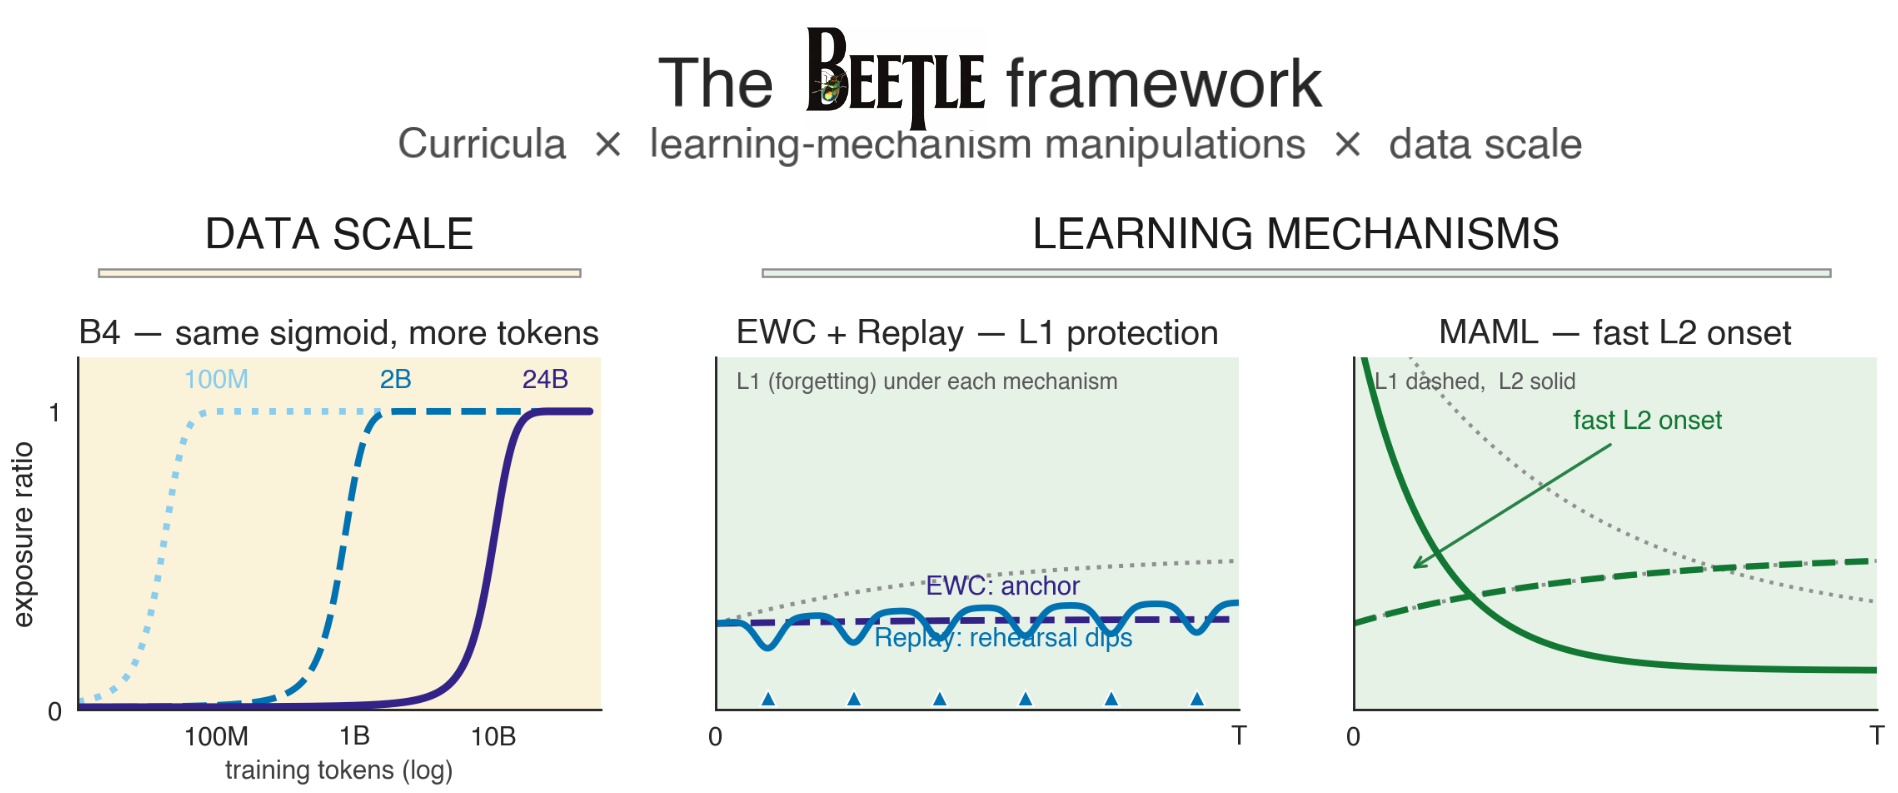
\includegraphics[width=0.85\linewidth]{fig/logo/3.png}
    \caption{Schematic comparison of the five \beetle{} bilingual exposure curricula B1--B5 (cf.\ Tab.~\ref{tab:curricula-overview}); the L1:L2 token-mix trajectory across training is rendered for each curriculum, with B2/B3/B5 sharing a sigmoid L2-onset and B4 a constant-mean-with-bursts schedule from step~0.}
    \label{fig:beetle}
\end{figure}


\begin{table}[!ht]
        \begin{tabular}{lccccc c}
        \toprule
        \textbf{Work} & \textbf{S} & \textbf{CL} & \textbf{M} & \textbf{C} & \textbf{CF} & \textbf{Dim} \\
        \midrule
        Constantinescu et al.\ (2025) & W & -- & -- & EWC & -- & $\triangle$ \\
        Arnett et al.\ (2025)         & W & -- & \checkmark & -- & -- & $\triangle\triangle$ \\
        Aoyama et al.\ (2024)         & W & -- & -- & -- & RT & $\triangle$ \\
        Diehl Martinez et al.\ (2025) & W & -- & -- & -- & -- & $\triangle\triangle$ \\
        Anon.\ (2025)                 & H & \checkmark & \checkmark & -- & -- & $\triangle\triangle\triangle$ \\
        Diehl Martinez et al.\ (2023) & H & \checkmark & -- & -- & -- & $\triangle\triangle\triangle$ \\
        Mita et al.\ (2025)           & H & -- & -- & -- & WM & $\triangle\triangle$ \\
        \midrule
        \textbf{BeetleLM}
        & \textbf{H+W}
        & \checkmark
        & \checkmark
        & \checkmark
        & \checkmark
        & $\triangle\times7$ \\
        \bottomrule
        \end{tabular}
\end{table}



\section{\beetle{} Training Framework}\label{sec:train}

\beetle{}, by default, uses on a custom \textsc{Pico} decoder stack \citep{diehl-martinez-etal-2025-pico} with curriculum-aware checkpointing, a registry of fifteen continual-learning strategies, and a tokeniser layer that supports per-language, shared-bilingual, and shared-trilingual vocabularies. 

\subsection{Architectural Variants}\label{sec:beetle-architecture-registry}

The body backbone is \texttt{PicoDecoder}, a LLaMA-style \citep{touvron2023llama} decoder with $L=14$ blocks, RMSNorm \citep{zhang2019rms}, grouped-query attention \citep{ainslie2023gqa} (12 query heads, 1 key/value head), rotary position embeddings \citep{su2024rope}, SwiGLU feed-forward \citep{shazeer2020glu} expanding to $4d$ and projecting back to $d$, vocabulary size $50{,}304$, sequence length $512$, BF16-mixed precision. Width is the only scale-dependent hyper-parameter: $d\in\{96,384,768,1536\}$ for the tiny, small, medium, and large variants. The 125M-parameter ``medium'' variant ($d=768$, 12 heads, 1 KV head, 14 layers) is used for every reported run. 

Complementary architectures enable controlled comparisons across inductive biases: \textbf{BGPT}, a GPT-2-style decoder with learned positional embeddings used in \citet{arnett-etal-2025-acquisition}; \textbf{BeetleMoE}, a top-$k$ mixture-of-experts model with ST-MoE auxiliary routing losses; \textbf{BeetleSSM}, which replaces attention blocks with Mamba-style state-space modules. Pre-pretraining (Shuffle-Dyck) and time-varying ALiBi slopes are implemented as opt-in cognitive-constraint overlays inside the registry and not used in headline runs.

\subsection{Continual-Learning Strategies}\label{sec:cl-strategies}

The \beetle{} pretraining library (\texttt{beetlelm}) contains  \textbf{fifteen} modular continual-learning strategies grouped into five families. Parameter regularisation: EWC \citep{kirkpatrick2017overcoming} with $\lambda\in[0,40]$ and Fisher snapshot at phase change, SI (synaptic intelligence), MAS (memory-aware synapses). Generative and similarity replay: LAMOL \citep{sun2020lamol} with $\lambda_{\text{replay}}\in[0,0.5]$, InsCL-style similarity replay (cosine and Wasserstein centroids), episodic-sample replay buffers. Meta-learning: first-order MAML / SMLMT \citep{bansal-etal-2020-self,africa-etal-2025-learning,africa-etal-2025-meta} with hybrid ratio $\in[0,0.4]$ and $N$-way/$k$-shot inner episodes. Distillation: feature-level (FitNets), output-level (Hinton-KD), and self-distillation against the pre-L2 anchor. Architectural and auxiliary-loss variants: TILT freeze-and-extend, exposure-LR plasticity boost (\texttt{plasticity\_boost}$\in[1,3]$), ALiBi-scheduler decay, Shuffle-Dyck pre-pretraining auxiliary loss. The B1--B5 grid reported in the body uses three of these (EWC, LAMOL, LR-plasticity); the remaining twelve are reproducible from the released \texttt{configs/continual\_learning/} YAML blocks. Tab.~\ref{tab:cl-registry} summarises the set of continual learning strategies.

\begin{table*}[t]
\centering
\small
\setlength{\tabcolsep}{3.5pt}
\begin{tabular}{llll}
\toprule
\textbf{Family} & \textbf{Strategy} & \textbf{Mechanism} & \textbf{Key hyperparameters} \\
\midrule
\multicolumn{4}{l}{\textit{Parameter regularisation}} \\
& EWC \citep{kirkpatrick2017overcoming} & Diagonal-Fisher quadratic penalty at phase change & $\lambda\in[0,40]$, $K_{\text{Fisher}}=10$ \\
& SI & Online importance accumulation & $c$, damping \\
& MAS & Gradient-magnitude importance & $\lambda$ \\
\midrule
\multicolumn{4}{l}{\textit{Replay}} \\
& LAMOL \citep{sun2020lamol} & Pseudo-sample generation, nucleus sampling & $\lambda_{\text{replay}}\in[0,0.5]$, top-$p$ \\
& InsCL similarity replay & Centroid-similarity weighted replay & cosine/Wasserstein, buffer size \\
& Episodic replay & Stored exemplars, uniform sampling & buffer size, mix ratio \\
\midrule
\multicolumn{4}{l}{\textit{Meta-learning}} \\
& MAML / SMLMT & Inner-loop adaptation on (S,Q) splits & hybrid ratio $\in[0,0.4]$, $N$-way, $k$-shot \\
\midrule
\multicolumn{4}{l}{\textit{Distillation}} \\
& Hinton-KD & Soft-target cross-entropy against pre-L2 anchor & $T$, $\lambda_{KD}$ \\
& Self-distillation & Same model as teacher at earlier checkpoint & ckpt offset \\
& FitNets feature distill. & Hidden-state $\ell_2$ alignment & layer-pair list \\
\midrule
\multicolumn{4}{l}{\textit{Architectural / auxiliary-loss}} \\
& TILT freeze-and-extend & Freeze backbone; train embed + LM head & frozen modules \\
& Exposure-LR plasticity & Token-exposure LR with phase-transition boost & boost $\in[1,3]$, warmup tokens \\
& ALiBi scheduler & Time-varying ALiBi slopes across phases & initial/final slope, decay shape \\
& Shuffle-Dyck pre-pretraining & Formal-language warmup before NL & steps, depth \\
& EWC + MAML stack & Composite of regularisation + meta-learning & paired hyperparameters \\
\bottomrule
\end{tabular}
\caption{The fifteen continual-learning strategies in the \beetle{} registry. The reported B1--B5 grid uses EWC, LAMOL, and exposure-LR plasticity overlays; the remaining twelve are reproducible from released YAML.}
\label{tab:cl-registry}
\end{table*}

\section{\beetle{} Curricula}\label{sec:beetle-curricula}

\paragraph{Bilingual conditions (B1--B5).} The five bilingual exposure schedules used in every reported run differ along three axes: \emph{L2 onset timing} (immediate / mid-training / late), \emph{final L1:L2 ratio} (50:50 / 80:20 / etc.), and \emph{transition sharpness} (sharp vs.\ sigmoid). \textbf{B1 Balanced}: 50:50 L1:L2 throughout (from step 0). \textbf{B2 Simultaneous}: 100\% L1 until 50\% of training, sigmoid ramp to 50:50. \textbf{B3 Sequential}: 100\% L1 until 50\% of training, then $\{0:100, 33:67, 50:50\}$ L1:L2 in three onset-ratio variants (B3-0 / B3-33 / B3-50). \textbf{B4 Classroom}: episodic L2 bursts with EWC overlay, 80:20 token budget. \textbf{B5 Late}: L2 introduced at 80\% of training. All conditions hold total token budget constant at the per-pair scale (100M HumanScale, 2B FineWeb-2B, 24B FineWeb-24B) and share the \texttt{PicoDecoder} backbone described in App.~\ref{sec:beetle-architecture-registry}.

\paragraph{Trilingual conditions (T1--T4).} \textbf{T1 Simultaneous Trilingual}: $\approx$33/33/33 mixture, context-clustered batches. \textbf{T2 Sequential Trilingual}: $L_1\to L_2\to L_3$ via chained sigmoids. \textbf{T3 Heritage~+ $L_3$}: $L_1\to L_2$ dominance $\to L_3$, with $L_1$ re-exposure. \textbf{T4 Dominant $L_2$ + Late $L_3$}: $L_2$ dominant, $L_1$ weak, $L_3$ introduced late. 

\paragraph{Formalisation.} A bilingual curriculum is a time-dependent mixture $\mathcal{D}_{\text{mix}}(t) = \alpha(t)\,\mathcal{D}_1 \cup (1-\alpha(t))\,\mathcal{D}_2$ where $\alpha(t)\in[0,1]$ is the per-step L2 sampling probability and $t\in[0,T]$ indexes training. The polyglot generalisation is a language-exposure vector $\boldsymbol{\alpha}(t)=(\alpha_1(t),\ldots,\alpha_N(t))$ with $\sum_i \alpha_i(t)=1$. Each schedule is a \texttt{DataMix} object mapping a normalised progress value $p\in[0,1]$ to a per-language sampling weight; phase boundaries are discrete events recorded in \texttt{DataPipelineState} and trigger EWC snapshots in continual-learning runs.

\paragraph{Phase-based curricula.} Rather than specifying $\boldsymbol{\alpha}(t)$ as an arbitrary continuous function, we represent curricula as a sequence of discrete phases $\mathcal{C} = \{(\tau_k^{\text{start}}, \tau_k^{\text{end}}, \mathbf{w}_k)\}_{k=1}^{K}$, where $\mathbf{w}_k \in \mathbb{R}^N$ is a language-weight vector satisfying $\sum_i w_{k,i}=1$. For training progress $t$ such that $\tau_k^{\text{start}} \le t/T < \tau_k^{\text{end}}$, we set $\boldsymbol{\alpha}(t) = \mathbf{w}_k$. This compact representation supports arbitrary multilingual mixtures and is the YAML-declarative form used in every released run.


\subsection{\beetle{} Control Parameters: Continual Learning and Catastrophic Forgetting}\label{sec:beetle-control-parameters}

\beetle{} allows the specification of more complex acquisition scenarios through schedule primitives. 

\begin{itemize}
    \item \textsc{ConstantExposure}, \textsc{SigmoidRamp}, \textsc{LinearRamp}, \textsc{BurstSchedule}, \textsc{CyclicalSchedule}, \textsc{CompositeSchedule}
    \item \textsc{EpisodicSampler} that groups consecutive batches into named contexts (\emph{home} vs.\ \emph{classroom}, etc.).
\end{itemize}

\subsubsection{Bilingual \beetle{} Continual Learning Results}\label{appcomp:cl}

\begin{figure*}[!ht]
    \centering
    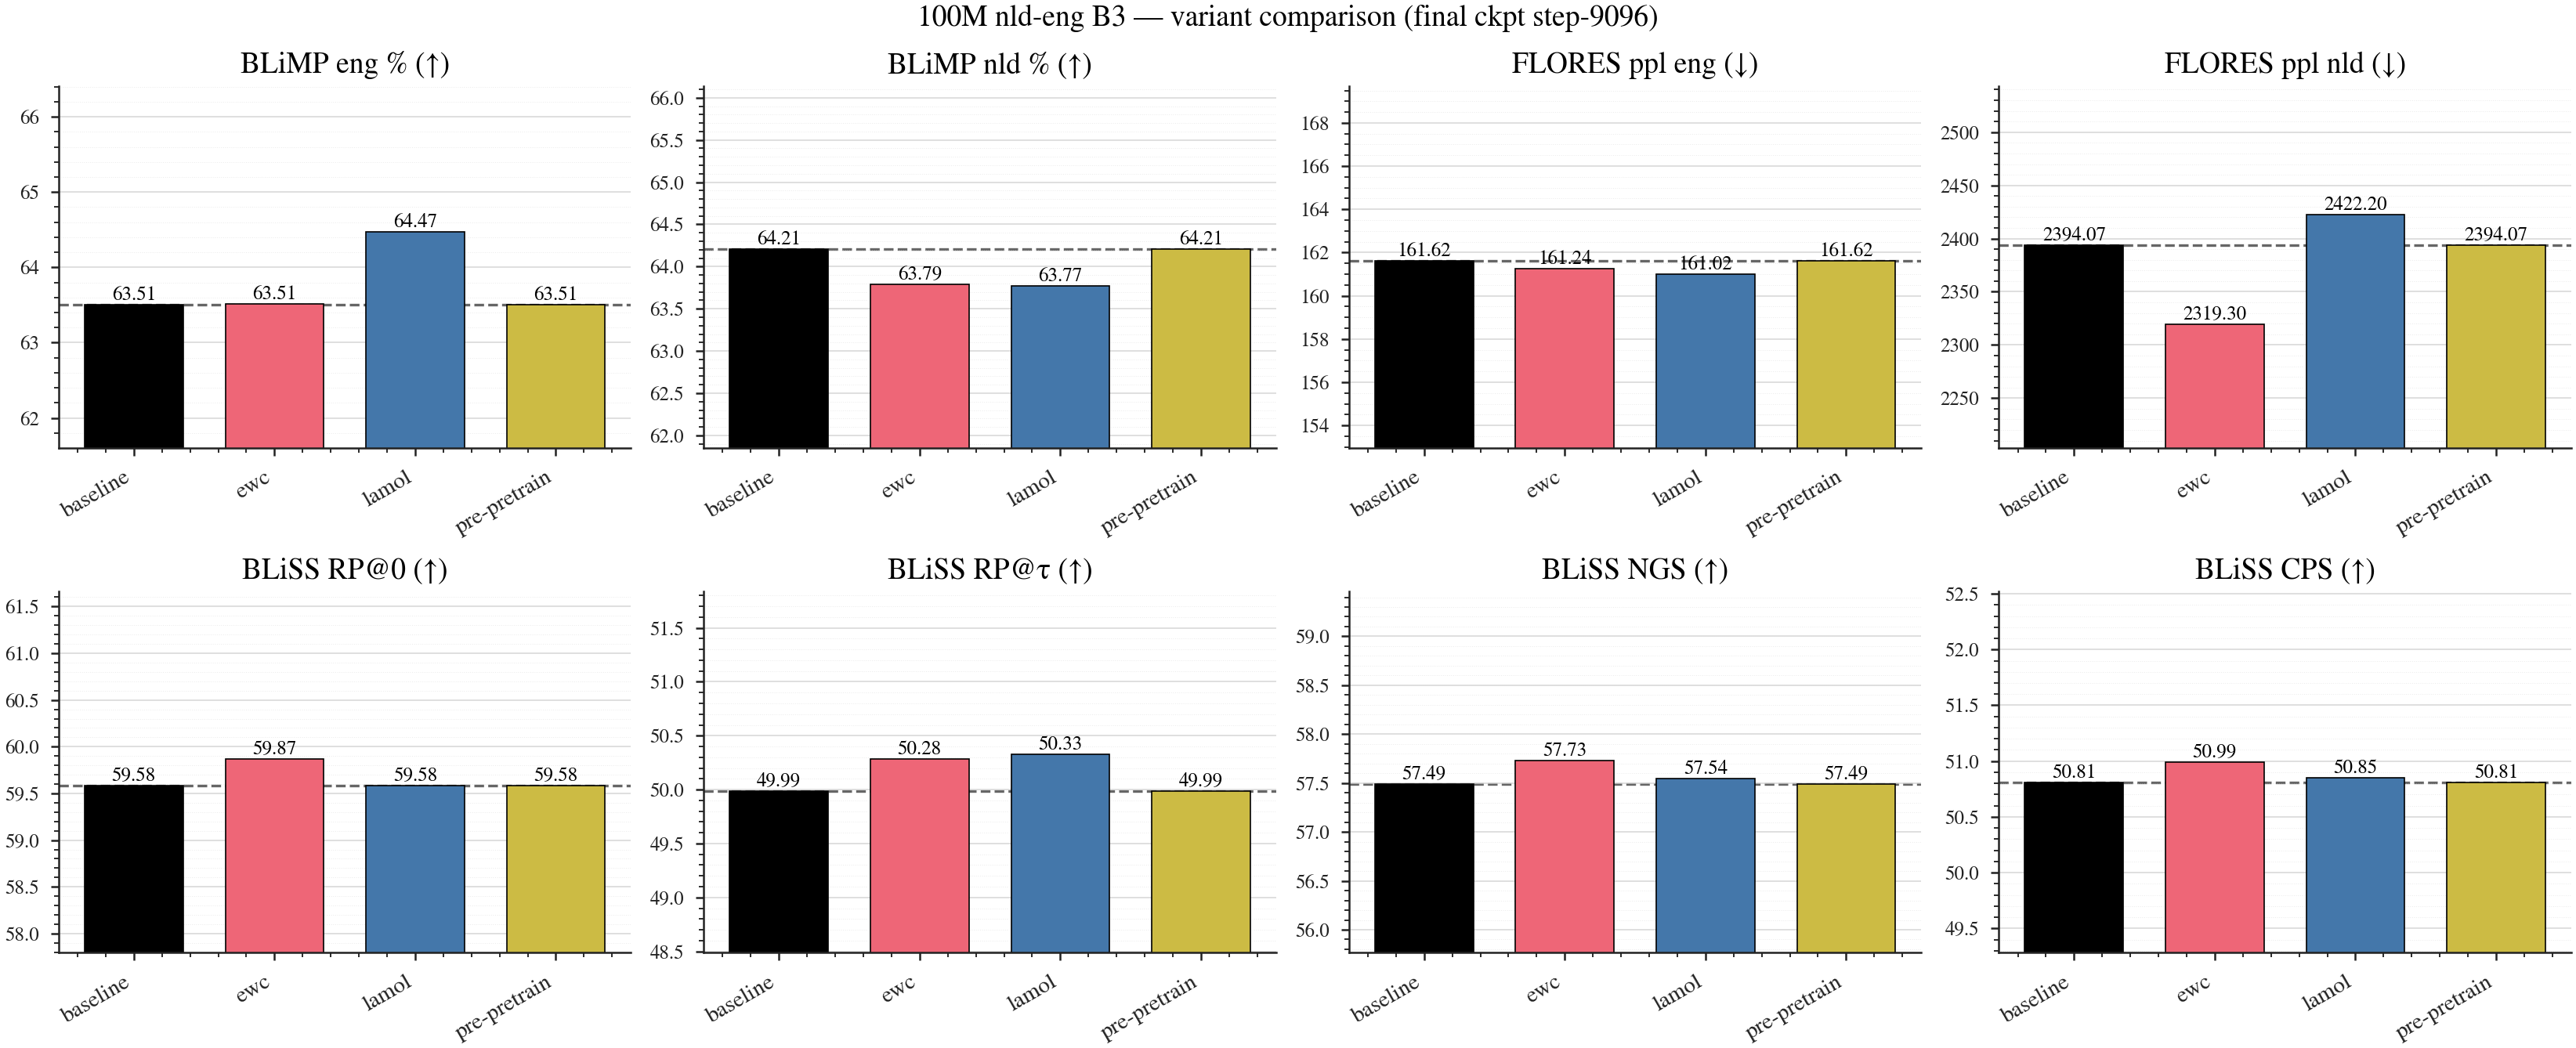
\includegraphics[width=0.86\linewidth,height=0.78\textheight,keepaspectratio]{fig/fig_variant_comparison_100m.png}
    \caption{\textbf{Continual-learning overlay comparison at \textsc{HumanScale}~100M.} BLiMP-eng, BLiMP-nl, BLiSS (RP@0 / RP@$\tau$ / NGS / CPS), and MECO~L2 alignment for five overlay variants (base, EWC, LAMOL, pre-pretrain, ALiBi) on the matched nld--eng cohort. Companion to Tab.~\ref{tab:strategy_results}; overlay effects fall within $\pm1.5$~pp of the base run on every axis.}
    \label{fig:cl_variant_comparison_100m}
\end{figure*}



\subsubsection{Human-Scale Trilingual CL Results [from earlier CDL experiments]}

All continual-learning experiments fix the language order to English~$\to$~Dutch~$\to$~Chinese under a uniform trilingual \texttt{sequential} exposure schedule, using the same PicoDecoder architecture and training budget as the main sweep ($T_{\max}\!=\!30{,}578$ steps). For EWC, we vary the regularisation strength $\lambda\!\in\!\{5,\,20,\,50,\,150\}$; the values $\lambda\!=\!20$ and $\lambda\!=\!150$ replicate settings reported in \citep{constantinescu2025investigating}.  The Fisher diagonal $\hat{F}$ is estimated on $K\!=\!10$ held-out L1 batches at the L1$\to$L2 phase boundary, and the anchor parameters~$\theta^*$ are snapshotted at the same moment; the penalty is then active for the remainder of training. For MAML, we vary the hybrid ratio $r\!\in\!\{0.25,\,0.50,\,0.75,\,1.00\}$, which controls the fraction of training steps executed as $N$-way, $K$-shot meta episodes ($N\!=\!5$, $K\!=\!1$, 3 inner SGD steps at $\alpha\!=\!0.1$) versus standard autoregressive steps. We have a combined condition that combines all four EWC strengths with all four hybrid ratios, yielding a $4\!\times\!4$ factorial design, which we compare against a trilingual baseline, producing 25 experimental conditions, each trained and evaluated identically to the baseline trilingual run.




\subsection{Meta-Learning}

\beetle{}  uses the \texttt{pico-maml} implementation of MAML used in \citet{africa-etal-2025-learning} and \citet{africa-etal-2025-meta}. 


\begin{algorithm}\small \caption{Distributed SMLMT Loop}\label{alg:dist-maml} \begin{algorithmic} \State Initialize model $f_\theta$, head $h_\phi$, outer optimizer, and inner SGD on $h_\phi$ \State step $\leftarrow 0$ \For{each sub-batch $B$ from dataloader} \State $X \leftarrow \text{AllGather}(B\ \text{inputs})$ \Comment{across devices} \State $r \leftarrow \text{Broadcast}(\text{Uniform}(0,1))$ \If{$r < \rho$} \State $(S,Q,y_S,y_Q) \leftarrow \text{MaskTokens}(X)$ \State $\phi_{\text{snap}} \leftarrow \phi$ \Comment{save head params} \For{$t = 1$ to $T_{\text{inner}}$} \State $\ell_S \leftarrow \text{CE}\big(h_\phi(f_\theta(S)),,y_S\big)$ \State $\phi \leftarrow \phi - \alpha,\nabla_\phi \ell_S$ \EndFor \State $\ell \leftarrow \text{CE}\big(h_\phi(f_\theta(Q)),,y_Q\big)$ \State $\phi \leftarrow \phi_{\text{snap}}$ \Comment{restore head} \Else \State $X_{\text{in}} \leftarrow X$ without last token; $Y \leftarrow X$ without first token \State $\ell \leftarrow \text{CE}\big(f_\theta(X_{\text{in}}),,Y\big)$ \EndIf \State Backward$\big(\ell ,/, \text{accum\_steps}\big)$ \If{$( \text{step} + 1 ) \bmod \text{accum\_steps} = 0$} \State OptimizerStep(); SchedulerStep(); ZeroGrad() \State AggregateMetrics($\ell$); Barrier() \EndIf \State step $\leftarrow$ step $+ 1$ \EndFor \end{algorithmic} \end{algorithm}

\begin{algorithm}\small \caption{Distributed AR Loop}\label{alg:dist-ar} \begin{algorithmic} \State Initialize configs, Fabric/strategy, tokenizer, model $f_\theta$, optimizer \State Prepare dataloader and distribute it \State step $\leftarrow 0$; ZeroGrad() \For{each sub-batch $B$ from dataloader} \State $X \leftarrow \text{AllGather}(B\ \text{inputs})$ \Comment{across devices} \State $X_{\text{in}} \leftarrow X$ without last token; $Y \leftarrow X$ without first token \State $\ell \leftarrow \text{CE}\big(f_\theta(X_{\text{in}}),,Y\big)$ \State Backward$\big(\ell ,/, \text{accum\_steps}\big)$ \If{$( \text{step} + 1 ) \bmod \text{accum\_steps} = 0$} \State OptimizerStep(); SchedulerStep(); ZeroGrad() \State Barrier() \Comment{optional} \EndIf \State step $\leftarrow$ step $+ 1$ \EndFor \end{algorithmic} \end{algorithm}



\subsection{Training Ablations}


\paragraph{Ablation grid.} Tab.~\ref{tab:ablation-sweep} enumerates the eight nld--eng \textsc{HumanScale} variants that constitute the minimal seed-grid ablation. Each variant is trained under three a-priori-fixed seeds $\{13, 42, 97\}$ to support a paired permutation test plus Cohen's $d_z$ with Holm--Bonferroni correction on the MECO~L2 alignment metric, executed by \texttt{analyze/significance\_ablation.py}. The full script trains all $8\times 3$ cells; the seed-delta script (\texttt{seeds\_13\_97}) trains only the remaining $8\times 2$ cells assuming seed 42 is already covered. Each variant trains on $8\times$A100 80~GB for $\sim$1~h.

\begin{table}[t]
\centering
\small
\caption{Minimal B1/B2/B3 ablation sweep on the nld--eng \textsc{HumanScale} pair. Eight variants $\times$ three seeds support paired-permutation significance tests on MECO~L2 $\Delta\log L$. LAMOL variants use $\lambda_{\text{replay}}=0.2$.}
\label{tab:ablation-sweep}
\begin{tabular}{@{}l l l l@{}}
\toprule
Family & Variant & Manipulation (vs.\ base condition) & Repo-slug suffix \\
\midrule
B1 & \textbf{B1}        & Base balanced (50:50 throughout)          & \texttt{balanced-b1} \\
B1 & \textbf{B1b}       & Balanced with delayed L2 onset variant    & \texttt{balanced-b1-delayed} \\
\midrule
B2 & \textbf{B2}        & Base simultaneous (sigmoid ramp from 50\%) & \texttt{simultaneous-b2} \\
B2 & \textbf{B2\_ewc}   & + EWC regulariser at phase change         & \texttt{simultaneous-b2-ewc-l\{$\lambda$\}} \\
B2 & \textbf{B2\_lamol} & + LAMOL generative replay ($\lambda=0.2$) & \texttt{simultaneous-b2-lamol-l20} \\
B2 & \textbf{B2\_lr}    & + LR-plasticity boost at L2 onset         & \texttt{simultaneous-b2-lr-b\{$k$\}} \\
\midrule
B3 & \textbf{B3}        & Base sequential (33:67 after phase transition) & \texttt{sequential-33-67-b3} \\
B3 & \textbf{B3\_full}  & Sequential with full EWC + MAML + LR stack & \texttt{sequential-33-67-b3-ewc-maml-lr} \\
\bottomrule
\end{tabular}

\vspace{0.5em}
\begin{tabular}{@{}l l l l@{}}
\toprule
Script & Seeds trained & Runs & Wall-clock \\
\midrule
\texttt{ablation\_minimal\_nld\_eng.sh}        & 13, 42, 97 & $8\times 3 = 24$ & $\sim$24\,h \\
\texttt{ablation\_minimal\_nld\_eng\_seeds\_13\_97.sh} & 13, 97     & $8\times 2 = 16$ & $\sim$16\,h \\
\bottomrule
\end{tabular}
\end{table}



\section{\raisebox{-0.3em}{
\includegraphics[height=1.2em]{fig/logo/BeetleLM.png}} Analyze: Pico-Analyze Comparative Interpretability}\label{sec:beetle-analyze}

TO DO 
- add some info about the gradients, OV circuits etc 


\section{Detailed MECO Results}\label{sec:meco-results}

This appendix evaluates how bilingual training curricula affect alignment between language-model surprisal and human L2 reading times in MECO. The central result is that staged bilingual exposure (B2/B3/B5) consistently improves first-pass reading-time alignment relative to balanced exposure, especially for Germanic L1 readers, and that small matched bilinguals outperform much larger multilingual LLMs on this psycholinguistic criterion.

% ---------------------------------------------------------------------
\subsection{MECO metric and mixed-effects specification}\label{sec:meco-metric-app}

We quantify LM--human alignment as the improvement in mixed-effects model fit obtained by adding surprisal predictors to a baseline reading-time regression:
\[
\Delta\log L = \log L(\text{full}) - \log L(\text{baseline}).
\]
\textbf{Larger values indicate that model surprisal explains additional variance in MECO reading times beyond standard lexical covariates.} The full model adds current-word and spillover surprisal terms to a baseline that controls for word length, frequency, and position; both are \texttt{lme4} fits on the wave-1$+$wave-2 joined first-pass data (\texttt{firstrun.dur}), and the surprisal block is the only difference between them. Exact formulas:

\begin{equation}
\label{eq:full-model}
\mathrm{firstrun\_dur} \sim
\underbrace{\mathrm{scale}(\mathrm{Surprisal}) + \mathrm{scale}(\mathrm{Surprisal1p}) + \mathrm{scale}(\mathrm{Surprisal2p})}_{\text{surprisal block (full only)}}
+ \mathcal{C}
+ (1 + \mathcal{C} \mid \mathrm{subid})
\end{equation}
\begin{equation}
\label{eq:meco-spec}
\mathrm{firstrun\_dur} \sim
\mathcal{C}
+ (1 + \mathcal{C} \mid \mathrm{subid})
\end{equation}

\noindent $\mathcal{C}$ is the shared lexical-covariate block (word position, word length and frequency each with two prior-word lags), \texttt{Surprisal1p}/\texttt{2p} are surprisal lags, and \texttt{subid} is the participant; fits use \texttt{REML=FALSE} with uncorrelated by-subject random slopes, released as \texttt{stats/meco\_l2.Rmd}.\footnote{Per-language rankings (Tab.~\ref{tab:meco}) average $\Delta\log L$ over reader-L1s within each (model, L2-language) cell. The per-participant heatmap (Fig.~\ref{appcomp:fig_meco_l2_participants_heatmap}) and cross-curriculum bootstrap forest (Fig.~\ref{appcomp:F4_curriculum_meco_deltaLL}) confirm the headline gap is not driven by a few unusual readers.}\label{appcomp:meco}

% ---------------------------------------------------------------------
\subsection{Headline curriculum results}\label{sec:meco-headline-app}

\textbf{The observed differences are more strongly associated with curriculum structure than with scale alone.} Tab.~\ref{tab:meco_curriculum_matched} is the central result: each \beetle{} bilingual is trained on L1$\to$English and evaluated against the reading times of the matching L2 reader population. Staged curricula (B2/B3/B5) yield the strongest alignment on the Dutch and German cells, with sequential (B3-33) and late-onset (B5) highest; balanced exposure (B1) is consistently weakest on both Germanic readers. Chinese is mixed, with no curriculum ahead. Because each curriculum is currently represented by a single seed, these results establish a robust curriculum-associated effect but do not yet isolate the causal contribution of exposure timing from the optimization path a given schedule induces.

\begin{table}[!ht]
  \centering
  \small
  \caption{\textbf{Matched-L1 \beetle{} curriculum sweep on MECO~L2 $\Delta\log L$.} Each cell is the L1$\to$English model evaluated on the matching L2 reader population (\textsc{HumanScale} 100M unless noted). Bold marks the winning curriculum within each reader column.}
  \label{tab:meco_curriculum_matched}
  \begin{tabular}{lrrr}
    \toprule
    Curriculum & Dutch & German & Chinese \\
    \midrule
    B1 balanced       & 62  & 75  & 106 \\
    B2 simultaneous   & 135 & 166 & 100 \\
    B3-33 sequential  & \textbf{140} & \textbf{177} & 103 \\
    B4 classroom-20   & 122 & 141 & 99 \\
    B5 late-onset     & 138 & 168 & \textbf{115} \\
    \midrule
    \multicolumn{4}{l}{\textit{FineWeb 2B / 24B (where available)}} \\
    \midrule
    B1 nld--eng FW    & 47  & ---          & --- \\
    B2 nld--eng FW    & 96  & ---          & --- \\
    B2 deu--eng FW    & --- & \textbf{185} & --- \\
    B3-33 nld--eng FW & 75  & ---          & --- \\
    B5 nld--eng FW    & \textbf{81} & 171  & --- \\
    \bottomrule
  \end{tabular}
\end{table}

The same curriculum ordering appears across available training scales (Fig.~\ref{fig:fig1_scaling_x_curriculum}) and across the full training-L1 $\times$ scale grid wherever a run exists (Fig.~\ref{fig:fig9b_curriculum_sweep_matched}).

\begin{figure}[!ht]
    \centering
    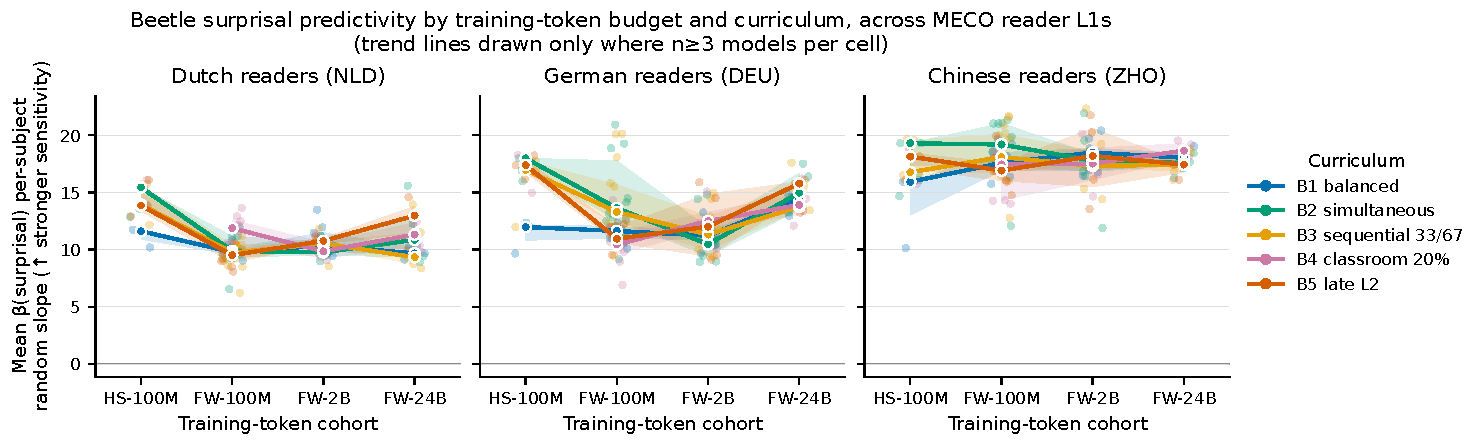
\includegraphics[width=1\linewidth]{fig/meco/fig1_scaling_x_curriculum.pdf}
    \caption{\textbf{Surprisal predictivity by training-token budget $\times$ curriculum.} Mean per-subject $\beta$(surprisal) random slope ($\uparrow$ stronger sensitivity) vs.\ training-token cohort (HumanScale~100\,M / FineWeb~2\,B / FineWeb~24\,B) for each curriculum (B1--B5; nld--eng, deu--eng), one panel per reader-L1. B3-33 and B5 maintain stronger per-token alignment than B1 across scales, with the largest separation on Germanic L1s.}
    \label{fig:fig1_scaling_x_curriculum}
\end{figure}

% ---------------------------------------------------------------------
\subsection{Comparison to multilingual baselines}\label{sec:meco-baselines-app}

\textbf{125M matched bilinguals outperform much larger multilingual LLMs on MECO alignment.} Tab.~\ref{tab:meco_baseline_comparators} sets the matched-L1 \beetle{} winner for each reader against the legacy BLOOM ladder (up to 7.1B) and a cohort of modern multilingual LLMs (up to 9B). On the Germanic readers the 125M matched bilingual is at or above every larger model; on Chinese it is competitive with the strongest legacy comparator. \textbf{Parameter count alone does not predict psycholinguistic alignment.}

\begin{table}[!ht]
  \centering
  \small
  \caption{\textbf{MECO~L2 $\Delta\log L$: \beetle{} matched bilinguals vs.\ baselines.} \beetle{} rows report the matched-L1 winner per reader (from Tab.~\ref{tab:meco_curriculum_matched}). Bold = best in column.}
  \label{tab:meco_baseline_comparators}
  \begin{tabular}{lrrrr}
    \toprule
    Model & Params & Dutch & German & Chinese \\
    \midrule
    \multicolumn{5}{l}{\textit{Legacy multilingual (BLOOM ladder)}} \\
    BLOOM-560m            & 0.56B & 44 & 182 & 149 \\
    BLOOM-1b1             & 1.1B  & 41 & 180 & \textbf{164} \\
    BLOOM-1b7             & 1.7B  & 34 & 151 & 137 \\
    BLOOM-7b1             & 7.1B  & 20 & 116 & 85 \\
    \midrule
    \multicolumn{5}{l}{\textit{Modern multilingual LLMs}} \\
    XGLM-4.5B             & 4.5B  & 9  & 19  & 23 \\
    EuroLLM-9B            & 9.0B  & 12 & 93  & 51 \\
    Gemma-2-9B            & 9.0B  & 9  & 97  & 50 \\
    Qwen-3-8B             & 8.0B  & 12 & 109 & 56 \\
    Llama-3.1-8B          & 8.0B  & 11 & 97  & 55 \\
    Baichuan-7B           & 7.0B  & 88 & 185 & 31 \\
    \midrule
    \multicolumn{5}{l}{\textit{\beetle{} matched bilinguals (125M)}} \\
    B3-33 nld--eng        & 0.125B & \textbf{140} & ---          & --- \\
    B3-33 deu--eng        & 0.125B & ---          & \textbf{177} & --- \\
    B2 deu--eng FW        & 0.125B & ---          & \textbf{185} & --- \\
    B5 zho--eng           & 0.125B & ---          & ---          & 115 \\
    \bottomrule
  \end{tabular}
\end{table}

Two figures make the comparison visual: the per-reader bar panel (Fig.~\ref{fig:meco_baselines_bars}) and the $\beta$-surprisal axis (Fig.~\ref{fig:bA5_beetle_vs_llm}).

\begin{figure}[!ht]
    \centering
    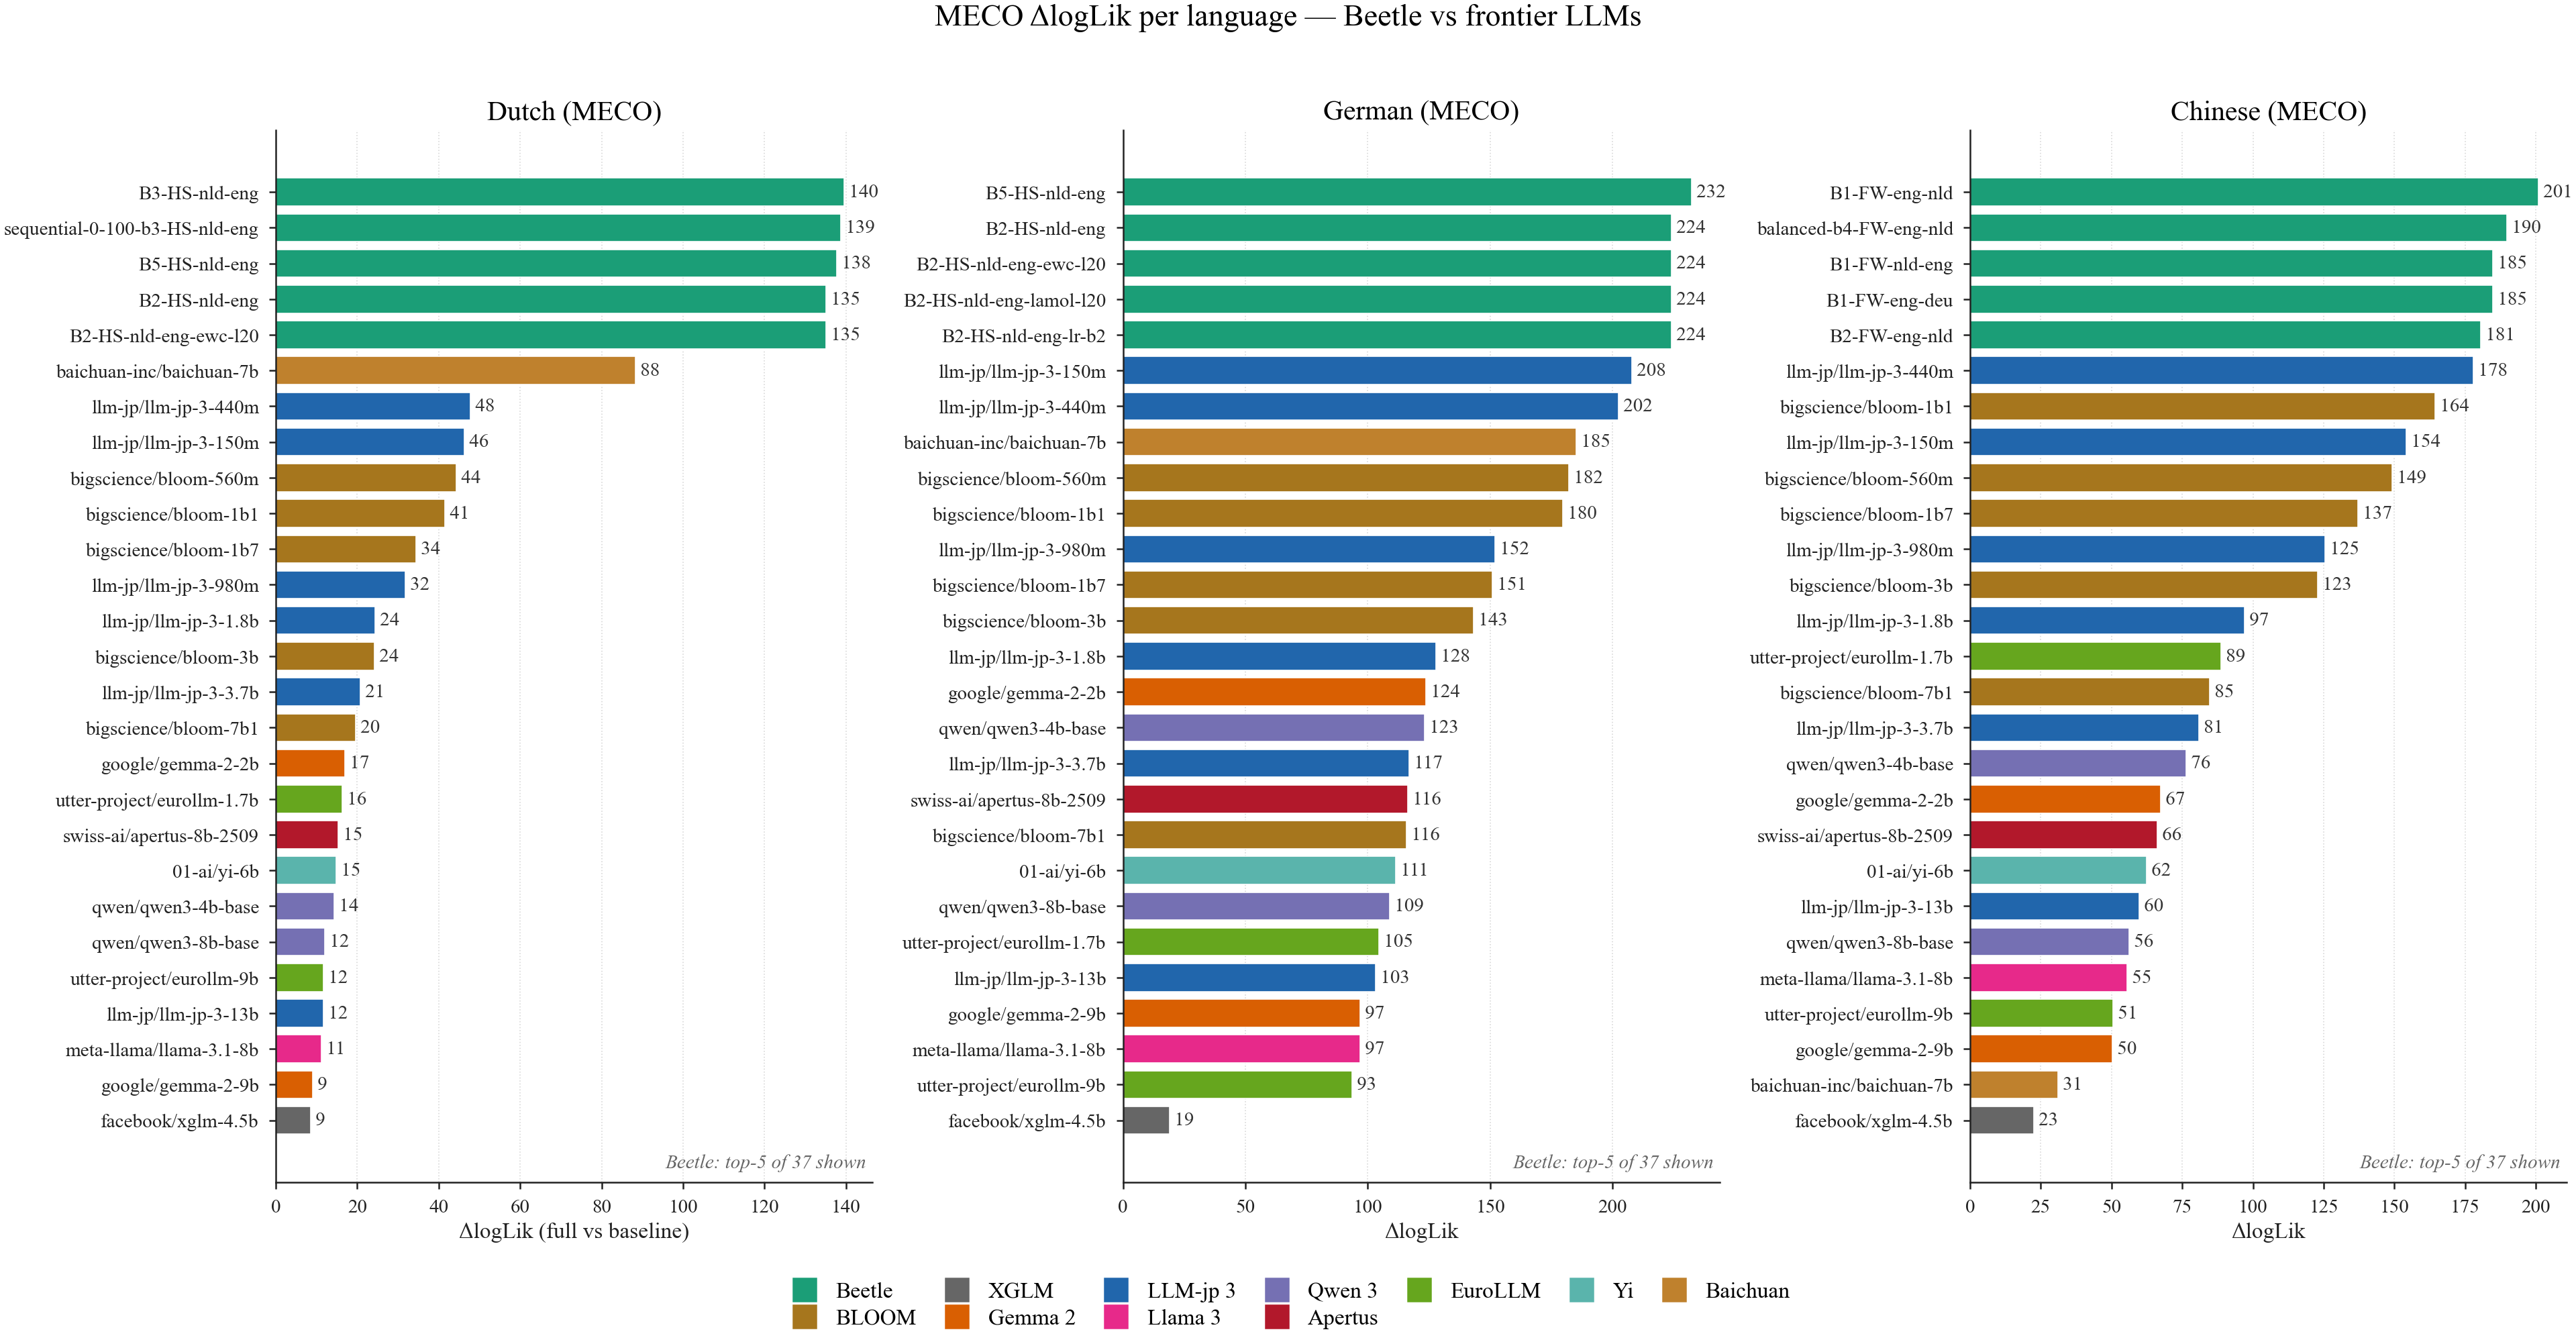
\includegraphics[width=1\linewidth]{fig/fig_meco_beetle_vs_baselines_bars.png}
    \caption{\textbf{MECO~L2 $\Delta\log L$ per reader-L1: \beetle{} vs.\ frontier LLMs.} One panel per reader-L1, grouped horizontal bars per model, ordered by descending $\Delta\log L$. Matched-bilingual \beetle{} bars cluster at the top of every Germanic-L1 panel; the modern bilingual LLM cohort trails them on every panel, including Chinese~L2.}
    \label{fig:meco_baselines_bars}
\end{figure}

\begin{figure}[!ht]
    \centering
    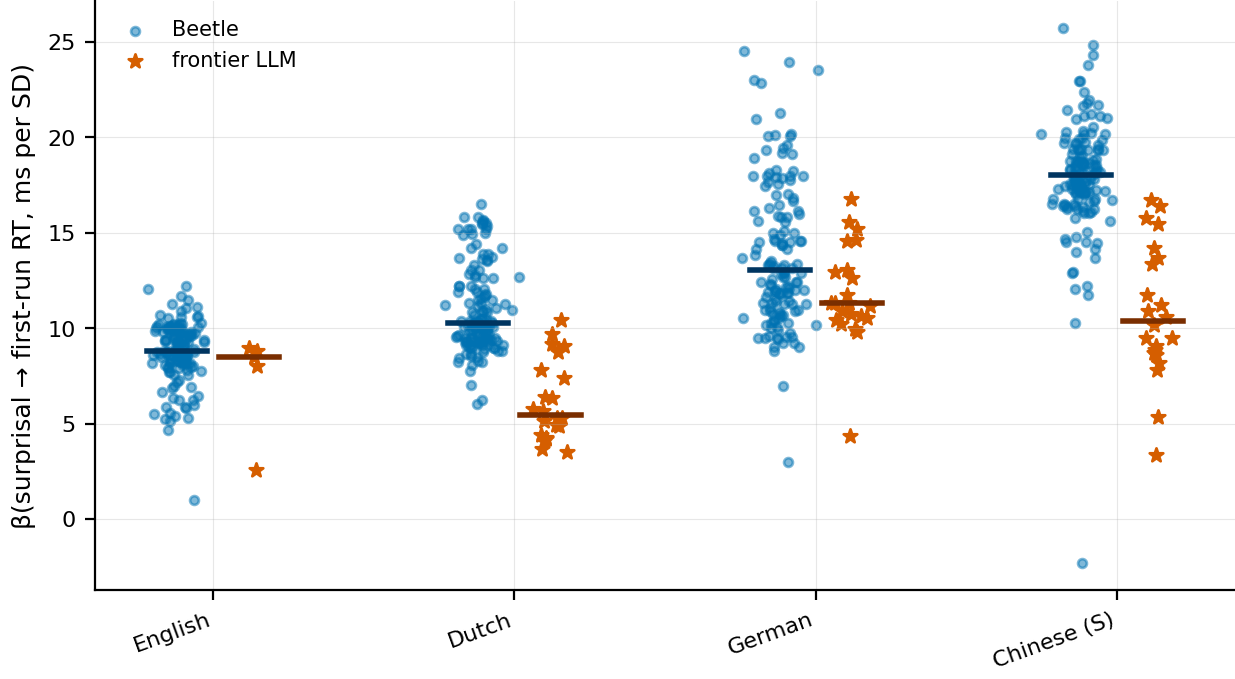
\includegraphics[width=1\linewidth]{fig/meco/bA5_beetle_vs_llm.png}
    \caption{\textbf{\beetle{} vs.\ frontier LLM on $\beta$-surprisal.} Per-curriculum $\beta$(surprisal) median for matched-bilingual \beetle{} 125\,M models (B1--B5; nld--eng, deu--eng, zho--eng) vs.\ four modern bilingual LLMs on the same reader-L1 cells. \emph{Note:} LLM bars use checkpoint-end values, since public checkpoints are not log-spaced.}
    \label{fig:bA5_beetle_vs_llm}
\end{figure}

% ---------------------------------------------------------------------
\subsection{Processing-stage dissociation}\label{sec:meco-stage-app}

\textbf{Staged curricula are associated with greater alignment on earlier lexical-access measures.} Relative to balanced exposure (B1), the simultaneous (B2), sequential (B3), and late-onset (B5) schedules \emph{improve} prediction of first-run duration (early lexical access) and \emph{worsen} prediction of refixations and regressions-in (late integration). B2 gains $+0.79$~SD on first-run duration (95\% CI $[+0.24, +1.33]$); B5 gains $+0.93$~SD ($[+0.43, +1.42]$). The matched late-measure interactions are uniformly negative (B2$\times$refixation $\beta^{z}={-}1.06$; B5$\times$regression $\beta^{z}={-}1.30$) and survive FDR correction.

The dissociation is not a bilingual-pretraining artefact. Against a same-architecture monolingual-English anchor under the same curriculum~$\times$~stage~$\times$~measure specification, B2 reaches monolingual first-run performance while B1 falls well short. Adding an English-competence covariate weakens the B2 late-measure effect but leaves the B5 dissociation strong (first-run $\beta^{z}={+}0.78$, $p{<}.001$; $\times$regression $-1.01$, $p{<}.001$). Late-onset exposure is the directionally most robust component of the interaction. The pattern reproduces in HumanScale~100M (B2 first-run $\beta^{z}={+}2.09$) and FineWeb~100M ($\beta^{z}={+}0.91$), so it is not specific to developmentally curated text.

The \textbf{B4 classroom condition} partially reproduces the staged effect at smaller magnitude (first-run $+0.40$~SD, refixation $-0.77$), consistent with a timing-sensitive interpretation in which the timing of L2 concentration matters more than the final exposure ratio.

Fig.~\ref{fig:fig3_spillover_decay} is the visual anchor: staged curricula concentrate the surprisal effect at lag~0 (early lexical access), whereas balanced B1 produces a flatter, lag-distributed profile characteristic of later integration.

\begin{figure}[!ht]
    \centering
    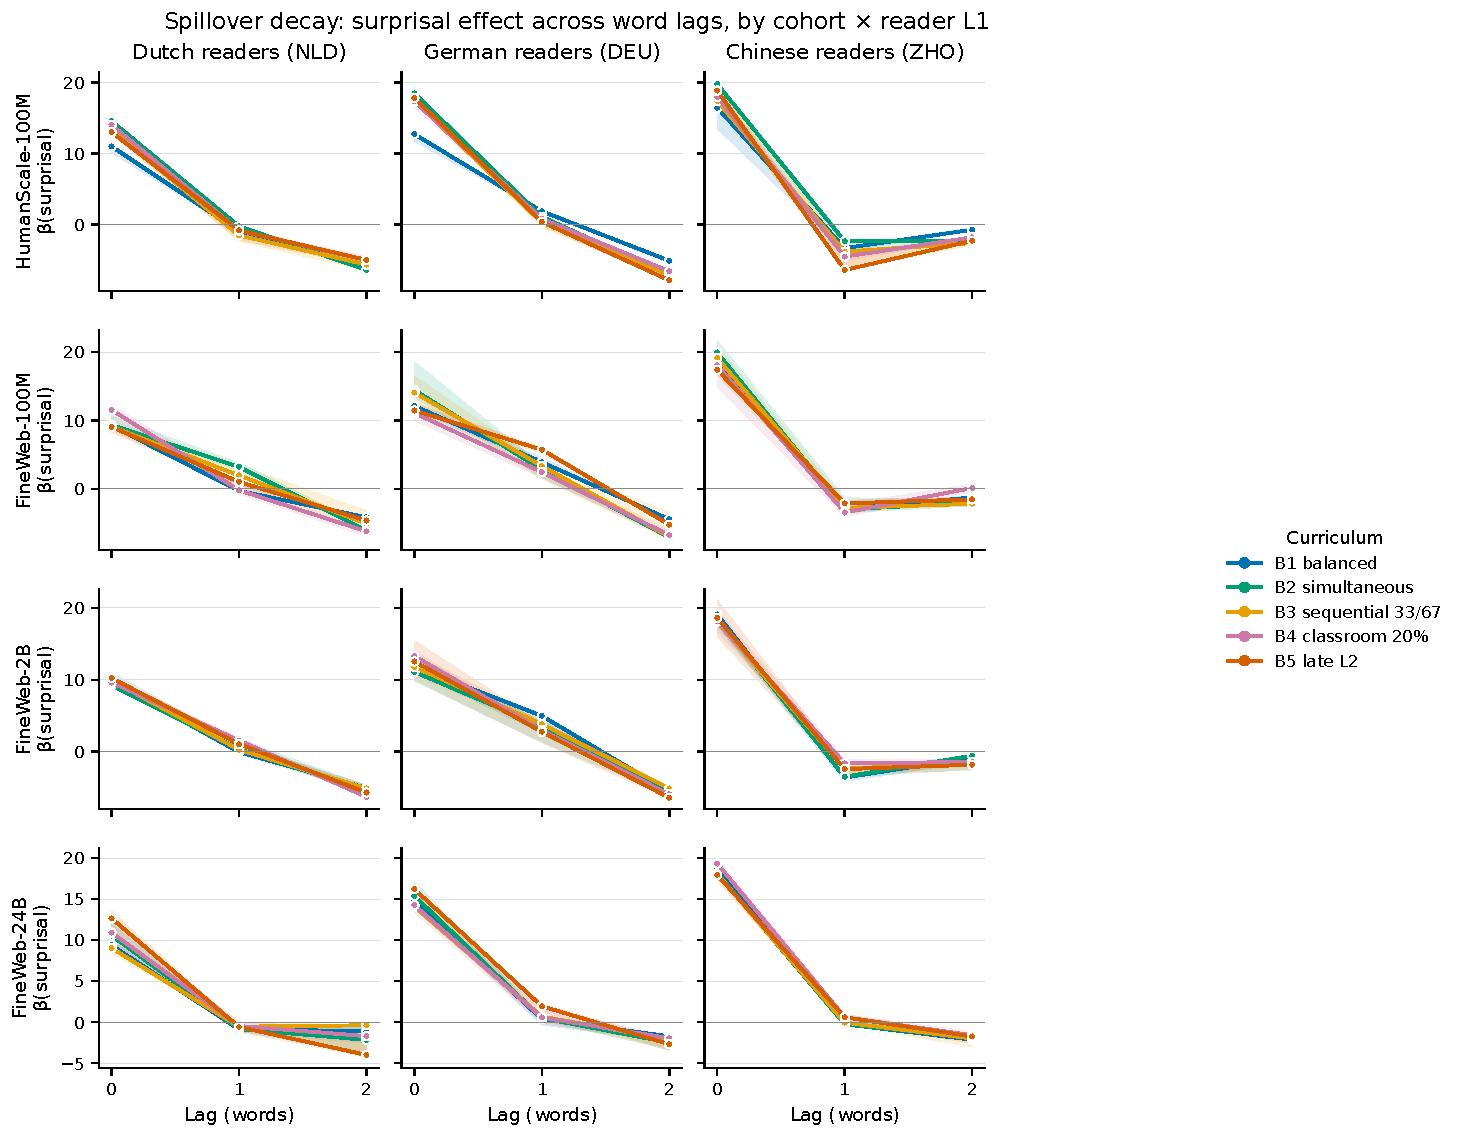
\includegraphics[width=1\linewidth]{fig/meco/fig3_spillover_decay.pdf}
    \caption{\textbf{Spillover decay: $\beta$(surprisal) across word lags.} Per (training-token cohort, reader-L1) cell, $\beta$(surprisal) at lags 0--3 on first-run duration. Staged curricula (B2/B3-33/B5) concentrate the effect at lag~0; balanced B1 produces a flatter, lag-distributed profile. Lag-0 dominance grows with training tokens for Germanic L1s.}
    \label{fig:fig3_spillover_decay}
\end{figure}

% ---------------------------------------------------------------------
\subsection{Mechanistic decomposition analyses}\label{sec:meco-mech-app}

\emph{This subsection is exploratory: it offers a candidate mechanism for the curriculum effect rather than establishing one, and no body claim depends on it.} The decomposition analysis tests the hypothesis that balanced curricula derive more predictive power from long-context surprisal, whereas staged curricula shift predictive mass toward shorter-horizon local and contextual predictors. The link to processing is direct: human first-pass reading times are dominated by rapidly available lexical expectations rather than discourse-scale integration, so a shift of surprisal variance toward shorter-horizon predictors is what we would expect to improve alignment with early lexical access.

We make this precise by splitting each model's reading-time predictive power into three additive, non-negative components --- a frequency component, a local-context ($k{=}4$-subword) component, and a long-context (full-passage) component --- via a nested-model likelihood decomposition; the contextual fraction of the total is the \emph{context-share} axis. Grouped by curriculum class (Tab.~\ref{tab:sig_decomp_curriculum}), staged curricula roughly halve the long-context share relative to balanced, and a context-truncation perturbation corroborates this (truncating to the last $k$ tokens degrades balanced surprisal more than staged).

A within-model intervention provides convergent, JFLEG-specific causal support (Fig.~\ref{fig:single-axis}): in a single FineWeb-2B nld--eng checkpoint, zeroing the top-50 SAE features most associated with context-share degrades the JFLEG margin $1.9$--$6.7\times$ more than ablating a matched frequency-feature control. The cross-task context-share correlations rest on $n{=}8$ and are reported in the analysis bundle.

\begin{figure}[!ht]
  \centering
  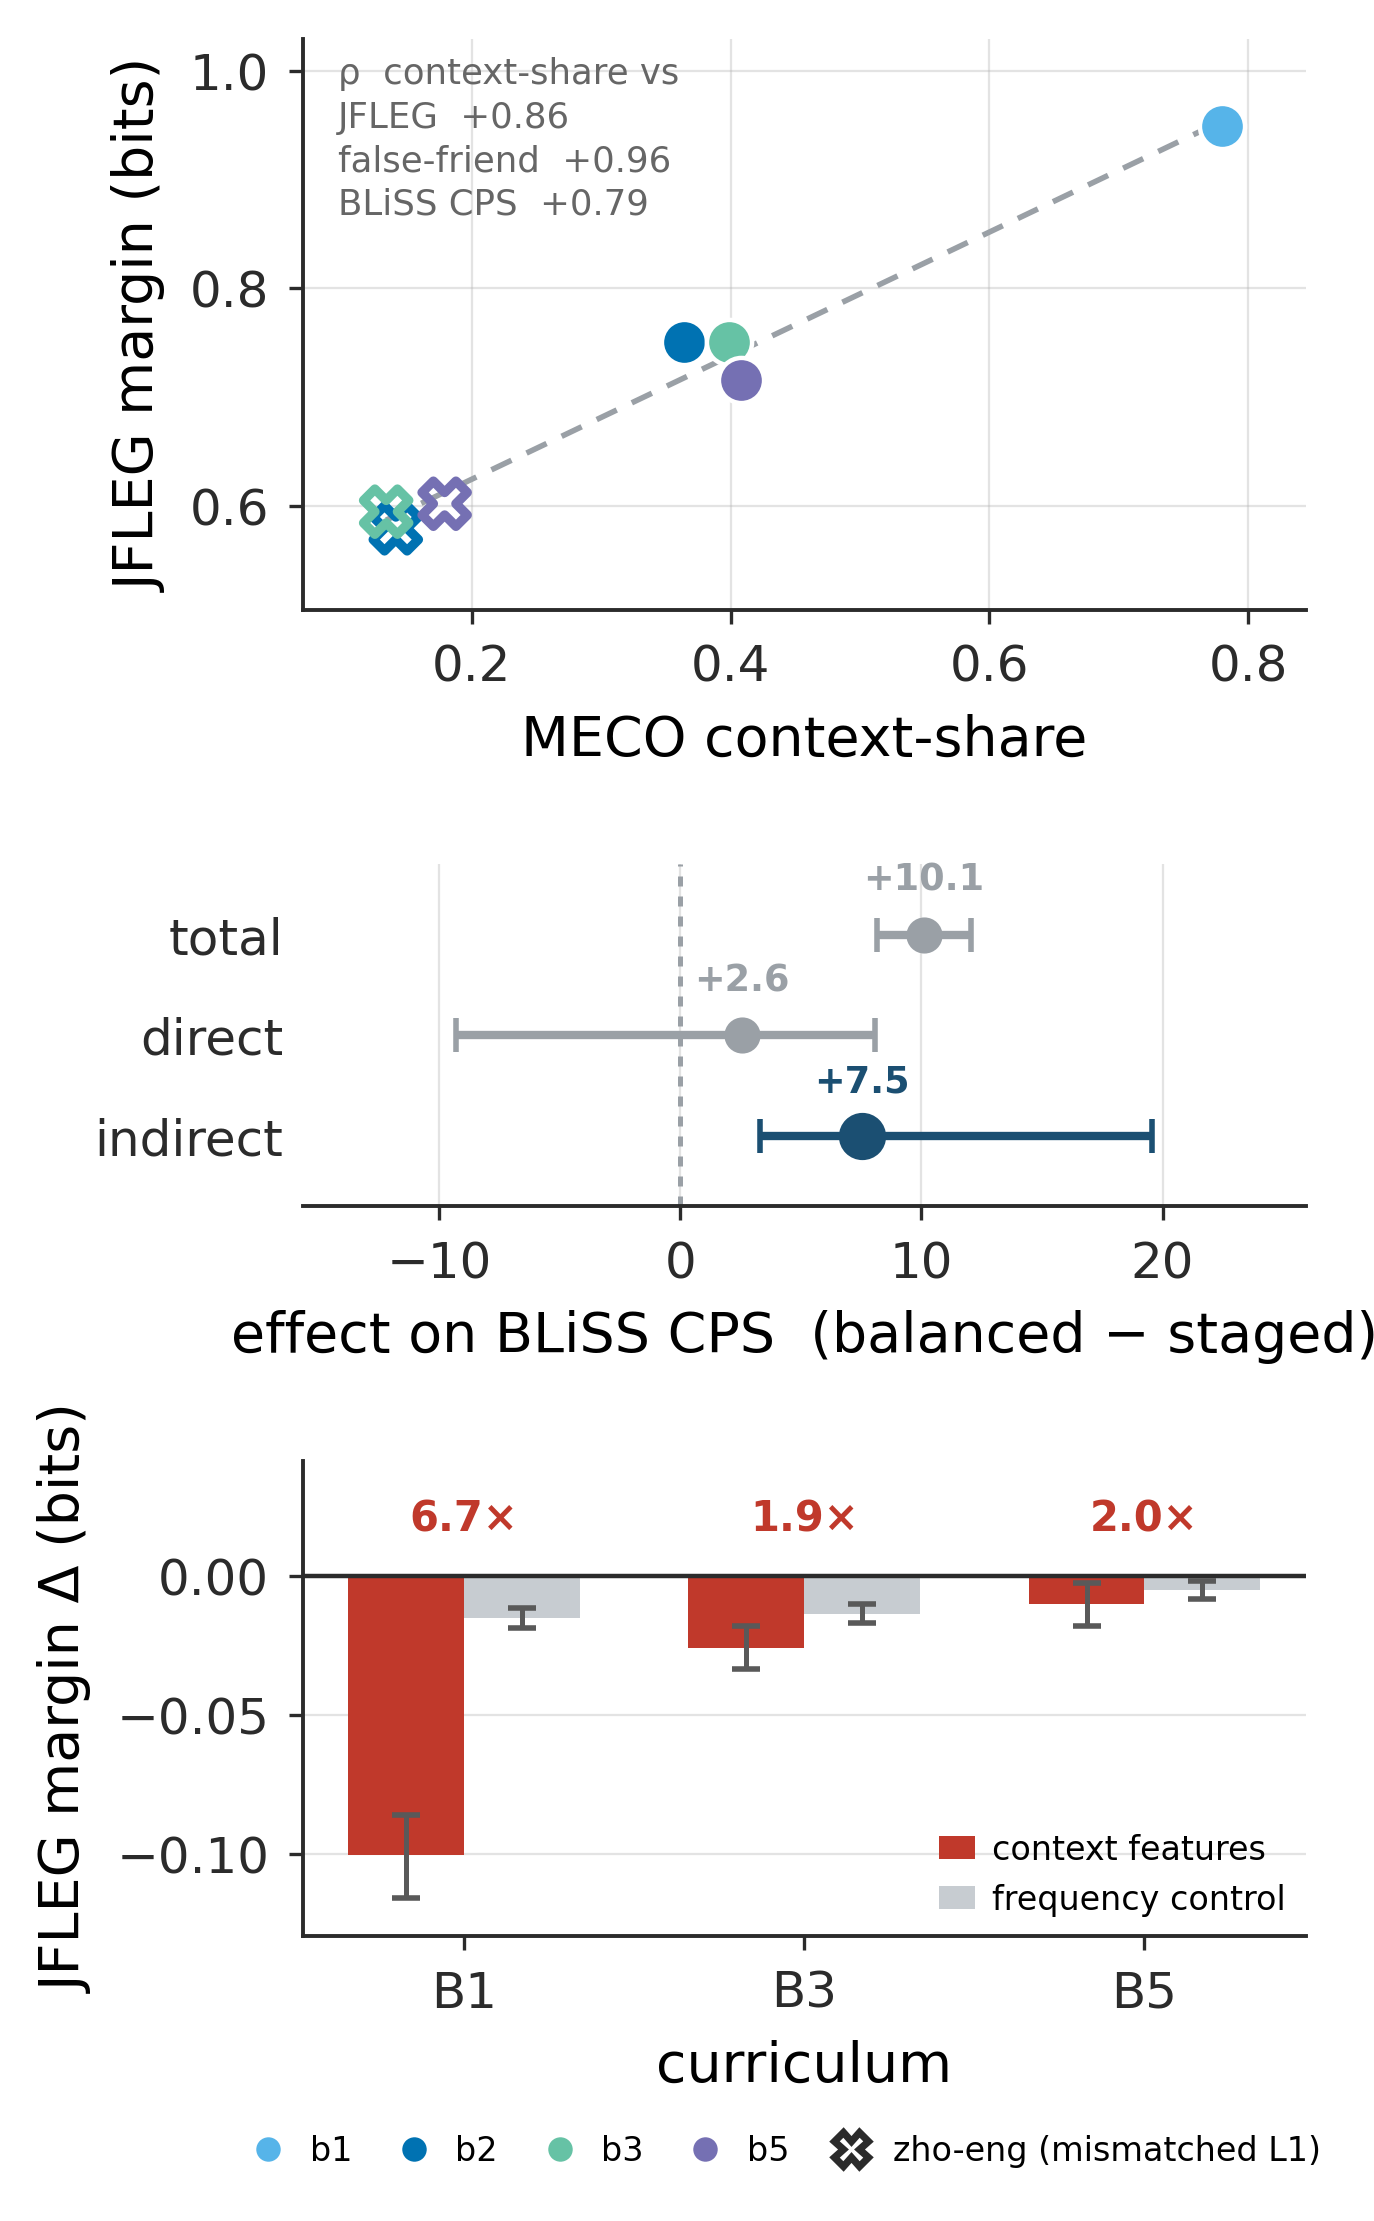
\includegraphics[width=\columnwidth]{fig/fig_single_axis_combined.png}
  \caption{\textbf{Within-model SAE causal test on JFLEG.} Zeroing the top-50 SAE features most associated with context-share degrades the JFLEG learner-fluency margin $1.9$--$6.7\times$ more than a matched frequency-feature control (every context CI excludes zero). Layer~8, FineWeb-2B nld--eng, single model; the causal test is JFLEG-specific.}
  \label{fig:single-axis}
\end{figure}

% ---------------------------------------------------------------------
\subsection{Canonical ledgers and audit artifacts}\label{sec:meco-canonical-app}

\emph{Archival / audit tables.} Tab.~\ref{tab:meco} is the compact canonical summary; the complete per-language and per-cell ledgers (equivalent to the released CSVs in the \texttt{beetle-analyze-meco} pipeline) are deposited in App.~\ref{sec:supp-tables} for reproducibility and do not bear on the narrative above. All cells are single-seed point estimates of Eq.~\ref{eq:meco-spec}; uncertainty is addressed centrally in \S\ref{sec:sig-uncertainty}.

\begin{table}[!ht]
  \centering
  \small
  \caption{Aggregated MECO~L2 $\Delta\log L$ headline cell (mean over reader-L1s within each L2 language). Bold marks the best model per L2 language.}
  \label{tab:meco}
  \begin{tabular}{lrrr}
    \toprule
    Model & Dutch L2 & German L2 & Chinese L2 \\
    \midrule
    BLOOM-1b1 (best legacy) & 41.5 & 179.7 & \textbf{164.3} \\
    BLOOM-7b1               & 19.7 & 115.9 & 84.7 \\
    XGLM-4.5B               & 8.7  & 19.0  & 22.6 \\
    \beetle{} best (per cell) & \textbf{139.6} & \textbf{184.7} & 115.4 \\
    \beetle{} canonical mean & \textbf{81.1} & 167.0 & 130.4 \\
    modern-bilingual aggr.\ mean & 12.3 & 97.5 & 56.3 \\
    \bottomrule
  \end{tabular}
\end{table}

% =====================================================================
\section{Statistical Significance Testing}\label{sec:significance-comprehensive}

This section reports the inferential ledger backing the body claims. The reproducibility entrypoints are \texttt{analyze/significance\_ablation.py} (ablation), \texttt{analyze/meco\_extended.py} and \texttt{analyze/run\_meco\_comparison.py} (Fisher~$z$, Wilcoxon, Friedman, mixed-effects), and \texttt{analyze/blimp\_significance.py} (BLiSS), all shipped with the released bundle (\texttt{results/archive/2026-04-18/}). The decisive tests are in \S\ref{sec:sig-core}; robustness and exploratory tests follow in \S\ref{sec:sig-robustness}; all uncertainty caveats and the family-correction policy are centralized in \S\ref{sec:sig-uncertainty}.

% ---------------------------------------------------------------------
\subsection{Core inferential tests}\label{sec:sig-core}

Three tests carry the cross-cohort and curriculum comparisons.

\paragraph{(1) Fisher $z$-test on coupling magnitude.} We test whether the \beetle{} bilingual cohort exhibits higher MECO~$\rho$ than each baseline class, with \beetle{} as reference ($n=512$ cells) and FDR-corrected two-sided $p$-values (Tab.~\ref{tab:sig_fisher}). Every comparison is highly significant with very large effect sizes (Cohen's $d\in[6.6,13.8]$): the \beetle{} cohort exceeds B-GPT, bilingual LLMs, the BLOOM ladder, and EuroLLM on $\bar\rho$.

\begin{table}[!ht]
  \centering
  \small
  \caption{\textbf{Fisher $z$-test, \beetle{} bilingual reference vs.\ each baseline class.} $n_\textsc{ref}=512$ cells; $p$ two-sided, FDR-corrected; $d$ on $z$-transformed $\rho$. Source: \texttt{meco\_baselines/fisher\_ztest.csv}.}
  \label{tab:sig_fisher}
  \begin{tabular}{lrrrr}
    \toprule
    Comparator & $\bar\rho_\textsc{ref}$ & $\bar\rho_\textsc{other}$ & $d$ & $p$ \\
    \midrule
    B-GPT           & 0.975 & 0.954 & 6.59  & $2.8{\times}10^{-29}$ \\
    bilingual LLMs  & 0.975 & 0.935 & 10.30 & $1.8{\times}10^{-6}$ \\
    BLOOM-ladder    & 0.975 & 0.911 & 13.79 & $1.5{\times}10^{-12}$ \\
    EuroLLM         & 0.975 & 0.937 & 9.93  & $6.7{\times}10^{-8}$ \\
    \bottomrule
  \end{tabular}
\end{table}

\paragraph{(2) Mixed-effects surprisal $\times$ model\_type interaction.} The cross-cohort test is a linear mixed-effects model with subject and sentence random intercepts and a fixed-effect surprisal~$\times$~\texttt{model\_type} interaction (Tab.~\ref{tab:sig_mixedlm_baselines}). Every baseline class shows a \emph{negative} interaction with $z$-surprisal --- it loses per-bit reading-time coupling relative to the \beetle{} reference --- with the BLOOM ladder losing the most ($\beta=-0.085$, $p<10^{-154}$).

\begin{table}[!ht]
  \centering
  \small
  \caption{\textbf{Baseline-anchored mixed-effects fit} (\beetle{} bilingual = reference level). Negative \texttt{zsurp}$\times$model interactions show each baseline loses MECO coupling relative to \beetle{}. Source: \texttt{meco\_baselines/mixedlm\_summary.csv}.}
  \label{tab:sig_mixedlm_baselines}
  \begin{tabular}{lrrr}
    \toprule
    Term & $\beta$ & SE & $p$ \\
    \midrule
    $z$-surprisal                          & $+0.464$ & 0.0017 & $<10^{-300}$ \\
    \quad $\times$ bilingual\_llm          & $-0.037$ & 0.0041 & $1.6{\times}10^{-19}$ \\
    \quad $\times$ bloom\_ladder           & $-0.085$ & 0.0032 & $4.0{\times}10^{-155}$ \\
    \quad $\times$ eurollm                 & $-0.038$ & 0.0036 & $9.0{\times}10^{-26}$ \\
    \quad $\times$ small\_bilingual        & $+0.063$ & 0.0017 & $3.5{\times}10^{-288}$ \\
    \bottomrule
  \end{tabular}
\end{table}

\paragraph{(3) Curriculum $\times$ processing-stage interaction.} The early-vs-late dissociation of \S\ref{sec:meco-stage-app} is backed by a peak-encoding depth test (Tab.~\ref{tab:sig_decomp_dissociation}): staged curricula peak at deeper layers than balanced for both stage bands, with the larger and more significant gap in the early-stage (first-fixation / first-run) band.

\begin{table}[!ht]
  \centering
  \small
  \caption{\textbf{Peak-encoding depth dissociation, balanced vs.\ staged.} Mann--Whitney on per-fit normalised peak layer depth (0=embedding, 1=output). Source: \texttt{meco\_detailed/dissociation\_model.csv}.}
  \label{tab:sig_decomp_dissociation}
  \begin{tabular}{lrrrr}
    \toprule
    Stage & $\overline{\text{peakfrac}}_\textsc{bal}$ & $\overline{\text{peakfrac}}_\textsc{stg}$ & $U$ & $p$ \\
    \midrule
    early (first-fix / first-run) & 0.702 & 0.809 & 6767.0 & $5.4{\times}10^{-6}$ \\
    late (refixation / regression) & 0.762 & 0.820 & 8055.5 & $5.5{\times}10^{-3}$ \\
    \bottomrule
  \end{tabular}
\end{table}

% ---------------------------------------------------------------------
\subsection{Robustness and exploratory tests}\label{sec:sig-robustness}

Additional robustness analyses are deposited with the released bundle and summarized here. The \textbf{decomposition tests} back \S\ref{sec:meco-mech-app}: a scale-pooled Mann--Whitney on per-fit ($\Delta\log L_\textsc{long}-\Delta\log L_\textsc{local}$) gives $U=7048.0$, $p=4.1{\times}10^{-3}$ (Tab.~\ref{tab:sig_decomp_curriculum}), and a model-level permutation test on the frequency-component share gives $\Delta=+0.364$, $p_\text{perm}=1.0{\times}10^{-4}$. The \textbf{within-family ablations} (paired permutation over three seeds, Holm-corrected) declare no winner at $\alpha=0.05$, which is why the body treats B2/B3/B5 as a class rather than naming a single variant. The \textbf{Friedman omnibus} confirms a positive surprisal--reading-time relation within each language band ($p<10^{-43}$), and the \textbf{pairwise Wilcoxon ledger} finds $2{,}159$ baseline-vs-\beetle{} comparisons significant at Holm-corrected $p<0.05$ with zero within-\beetle{} pairs rejecting. The \textbf{BLiSS per-cell binomials} show RP$@0$ above chance in the matched Germanic and Slavic families, with CPS the only metric inverting below chance under L2 schedules (\S\ref{sec:discrim-bliss}).

\begin{table}[!ht]
  \centering
  \small
  \caption{\textbf{Balanced vs.\ staged decomposition share (full N).} Staged schedules roughly halve the long-context share. Source: \texttt{meco\_detailed/decomp\_curriculum\_summary.csv}.}
  \label{tab:sig_decomp_curriculum}
  \begin{tabular}{lrrrr}
    \toprule
    Group & $n_\text{fits}$ & share$_\textsc{freq}$ & share$_\textsc{local}$ & share$_\textsc{long}$ \\
    \midrule
    balanced (B1)        & 63  & 0.126 & 0.457 & 0.417 \\
    staged (B2/B3-33/B5) & 180 & 0.395 & 0.399 & 0.206 \\
    \midrule
    \multicolumn{5}{l}{Mann--Whitney $U=7048.0$, $p=4.1{\times}10^{-3}$, $r=-0.243$}\\
    \bottomrule
  \end{tabular}
\end{table}

The mechanistic decomposition (\S\ref{sec:meco-mech-app}) is exploratory; its causal SAE evidence is restricted to a single model, layer, and task (JFLEG), and the cross-task context-share correlations rest on $n=8$ with wide bootstrap CIs. None of it is load-bearing for a body claim. The load-bearing curriculum reading is $\Delta\log L$ on \texttt{firstrun.dur}, backed by the three core tests of \S\ref{sec:sig-core}.

\paragraph{Family-correction policy.} Corrections are applied per family: within-family Holm for the ablation pairs and the pairwise Wilcoxon ledger; Benjamini--Hochberg FDR for the Fisher~$z$ cross-class comparisons and the Friedman omnibus; raw one-sided binomial for the per-cell BLiSS scores (the $160\times4$ family is left for the reviewer to correct as preferred); and uncorrected Mann--Whitney / permutation / mixed-effects for the decomposition tests, where each family contains only one or two scale-pooled tests and correction is uninformative. 


% ---------------------------------------------------------------------
\subsubsection{Caveats}\label{sec:sig-uncertainty}

\paragraph{Single-seed point estimates.} Except where a seed grid is explicitly named, every MECO and BLiSS cell in this appendix --- including \S\ref{sec:meco-canonical-app} --- is a single-seed point estimate. We do not report per-cell within-fit bootstrap CIs, because at one seed per cell the within-fit CI is not what discriminates between curricula; the relevant variance is between-seed. Seed-pretraining 

\paragraph{Planned seed-grid extension.} The pre-registered seed-grid extension (App.~\ref{sec:roadmap} item~5) widens the matrix to L1~$\times$~B-class~$\times$~scale and is the route to between-seed standard deviations and a per-cell bootstrap CI on every released readout. It is also what would (a) yield a Holm-corrected ablation winner per family, and (b) distinguish the timing, final-ratio, and trajectory-integral accounts of the B4 result.

\paragraph{Exploratory vs.\ load-bearing.} 



% =====================================================================
\section{Supplementary MECO Figures}\label{sec:meco-figs-supp}

Figs.~\ref{fig:fig1_scaling_x_curriculum}, \ref{fig:fig9b_curriculum_sweep_matched}, \ref{fig:meco_baselines_bars}, and \ref{fig:fig3_spillover_decay}.

\begin{figure}[!ht]
    \centering
    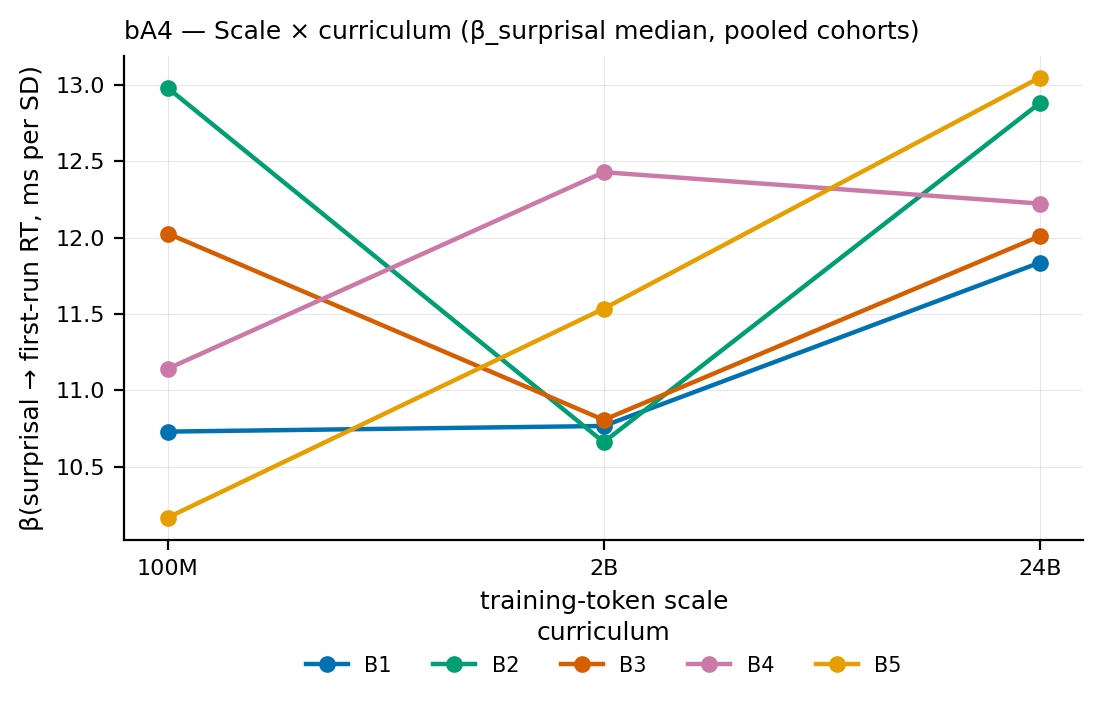
\includegraphics[width=1\linewidth]{fig/meco/bA4_scale_x_curriculum.png}
    \caption{\textbf{bA4 --- scale $\times$ curriculum on $\beta$-surprisal.} Median per-subject $\beta$(surprisal) random slope on first-run duration, pooled across reader L1s, vs.\ training-token cohort, one line per curriculum (B1--B5; nld--eng). The curriculum ordering is preserved across scale: staged curricula (B2/B3-33/B5) exceed balanced B1 at every available token budget.}
    \label{fig:bA4_scale_x_curriculum}
\end{figure}

\begin{figure}[!ht]
    \centering
    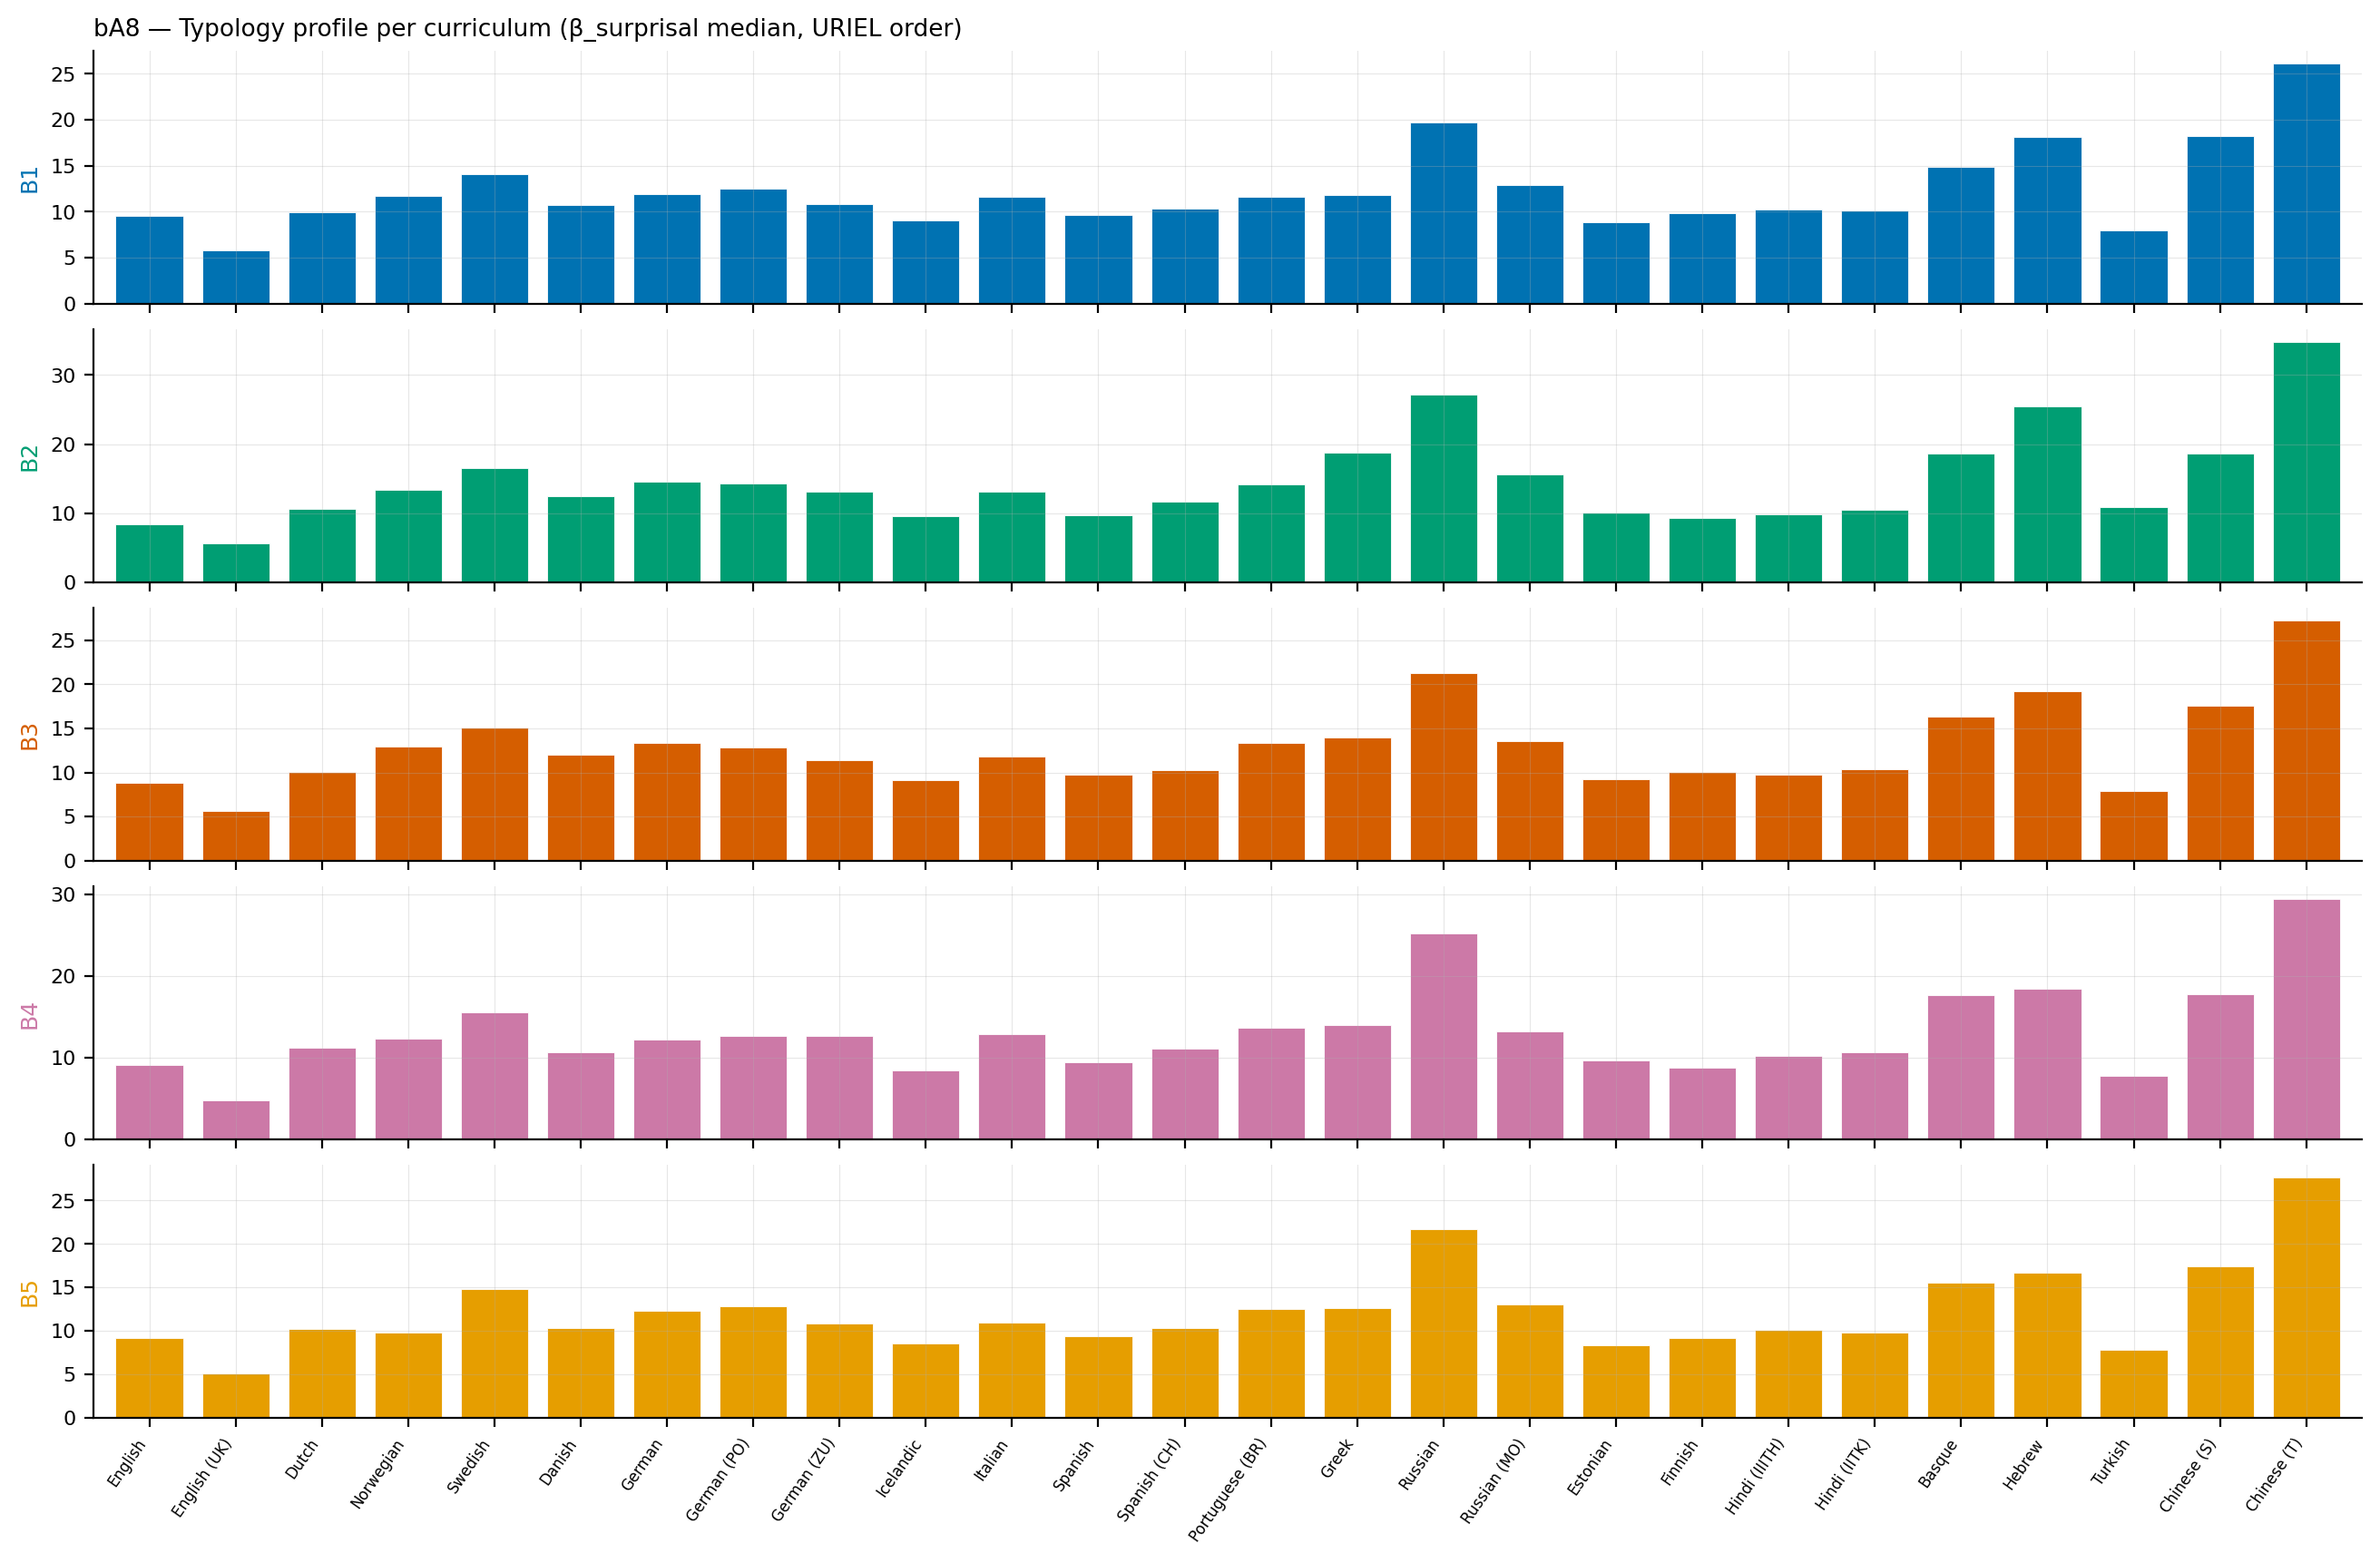
\includegraphics[width=1\linewidth]{fig/meco/bA8_typology_per_curriculum.png}
    \caption{\textbf{bA8 --- typological-distance profile per curriculum.} Per-curriculum profile of $\beta$(surprisal) across L1s ordered by URIEL distance from English (\textsc{nld}$<$\textsc{deu}$<$\textsc{spa}$<$\textsc{rus}$<$\textsc{fin/tur}$<$\textsc{heb}$<$\textsc{zho}). The B3-33 / B5 advantage concentrates on the L1-proximate Germanic cell and attenuates monotonically with typological distance, replicating the gradient on the $\Delta\log L$ axis.}
    \label{fig:bA8_typology_per_curriculum}
\end{figure}
\newpage
\clearpage 

% =====================================================================
\section{MECO Supplementary Tables}\label{sec:supp-tables}

Detailed per-model MECO results. 

%This section deposits the full MECO~L2 audit ledgers referenced from App.~\ref{sec:meco-canonical-app}. They reproduce the complete released CSVs of the \texttt{beetle-analyze-meco} pipeline and are provided for reproducibility only; every result discussed in the body and in App.~\ref{sec:meco-results} is carried by the compact tables there. All cells are single-seed point estimates of Eq.~\ref{eq:meco-spec}; uncertainty is addressed centrally in \S\ref{sec:sig-uncertainty}.

\begin{table*}[!ht]
  \centering
  \small
  \caption{\textbf{Canonical per-language MECO~L2 rows.} Per (model, L2-language) cell on the wave-1$+$wave-2 joined data: $\log L$ of the full model, of the baseline, and $\Delta\log L = \log L(\text{full}) - \log L(\text{baseline})$. Larger $\Delta\log L$ indicates better surprisal alignment. Only models with a plottable MECO row are included.}
  \label{tab:meco_langrows}
  \begin{tabular}{lrrrl}
    \toprule
    Model & $\log L$ & Baseline $\log L$ & $\Delta\log L$ & Class \\
    \midrule
    \multicolumn{5}{l}{\textit{Dutch (\texttt{nld})}} \\
    \midrule
    B-GPT nl-en simul. & $-193987.48$ & $-194075.73$ & $88.25$ & B-GPT \\
    XGLM-4.5b & $-194066.67$ & $-194075.32$ & $8.65$ & XGLM \\
    BLOOM-1b1 & $-194033.84$ & $-194075.32$ & $41.47$ & BLOOM \\
    BLOOM-1b7 & $-194040.91$ & $-194075.32$ & $34.41$ & BLOOM \\
    BLOOM-560m & $-194031.03$ & $-194075.32$ & $44.29$ & BLOOM \\
    BLOOM-7b1 & $-194055.62$ & $-194075.32$ & $19.69$ & BLOOM \\
    mono-nld & $-193979.29$ & $-194075.32$ & $96.02$ & mono-NLD \\
    mono-eng & $-194010.19$ & $-194075.32$ & $65.13$ & mono-ENG \\
    B1 eng-nld FW (FW) & $-194035.16$ & $-194075.32$ & $40.16$ & L2 bal. \\
    B1 nld-eng FW (FW) & $-194028.69$ & $-194075.32$ & $46.62$ & L2 bal. \\
    B1 nld-eng HS (HS) & $-194012.99$ & $-194075.32$ & $62.33$ & L2 bal. \\
    episodic nld-eng HS (HS) & $-194021.76$ & $-194075.32$ & $53.55$ & L2 bal. \\
    B2 eng-nld FW (FW) & $-194034.54$ & $-194075.32$ & $40.78$ & L2 sim. \\
    B2 nld-eng FW (FW) & $-193979.34$ & $-194075.32$ & $95.97$ & L2 sim. \\
    B2 nld-eng HS (HS) & $-193940.18$ & $-194075.32$ & $135.14$ & L2 sim. \\
    B3-0 nld-eng HS (HS) & $-193936.56$ & $-194075.32$ & $138.75$ & L2 seq. \\
    B3-33 eng-nld FW (FW) & $-194035.66$ & $-194075.32$ & $39.66$ & L2 seq. \\
    B3-33 nld-eng FW (FW) & $-193999.94$ & $-194075.32$ & $75.37$ & L2 seq. \\
    B3-33 nld-eng HS (HS) & $-193935.73$ & $-194075.32$ & $139.58$ & L2 seq. \\
    B4 nld-eng HS (HS) & $-193953.55$ & $-194075.32$ & $121.77$ & L2 class. \\
    B5 nld-eng HS (HS) & $-193937.57$ & $-194075.32$ & $137.74$ & L2 late \\
    \midrule
    \multicolumn{5}{l}{\textit{Chinese (\texttt{zho})}} \\
    \midrule
    B-GPT nl-en simul. & $-233899.84$ & $-234121.45$ & $221.61$ & B-GPT \\
    XGLM-4.5b & $-234098.92$ & $-234121.53$ & $22.60$ & XGLM \\
    BLOOM-1b1 & $-233957.22$ & $-234121.53$ & $164.30$ & BLOOM \\
    BLOOM-1b7 & $-233984.47$ & $-234121.53$ & $137.06$ & BLOOM \\
    BLOOM-560m & $-233972.28$ & $-234121.53$ & $149.25$ & BLOOM \\
    BLOOM-7b1 & $-234036.80$ & $-234121.53$ & $84.73$ & BLOOM \\
    mono-zho & $-234116.14$ & $-234121.53$ & $5.39$ & mono-ZHO \\
    mono-eng & $-234070.70$ & $-234121.53$ & $50.83$ & mono-ENG \\
    B1 zho-eng HS (HS) & $-234015.83$ & $-234121.53$ & $105.69$ & L2 bal. \\
    B2 zho-eng HS (HS) & $-234021.38$ & $-234121.53$ & $100.14$ & L2 sim. \\
    B3-33 zho-eng HS (HS) & $-234018.37$ & $-234121.53$ & $103.15$ & L2 seq. \\
    B4 zho-eng HS (HS) & $-234022.81$ & $-234121.53$ & $98.71$ & L2 class. \\
    B5 zho-eng HS (HS) & $-234006.13$ & $-234121.53$ & $115.40$ & L2 late \\
    \midrule
    \multicolumn{5}{l}{\textit{German (\texttt{deu})}} \\
    \midrule
    B-GPT nl-en simul. & $-275130.72$ & $-275373.70$ & $243.00$ & B-GPT \\
    XGLM-4.5b & $-275354.57$ & $-275373.57$ & $19.00$ & XGLM \\
    BLOOM-1b1 & $-275193.91$ & $-275373.57$ & $179.66$ & BLOOM \\
    BLOOM-1b7 & $-275222.85$ & $-275373.57$ & $150.71$ & BLOOM \\
    BLOOM-560m & $-275191.60$ & $-275373.57$ & $181.96$ & BLOOM \\
    BLOOM-7b1 & $-275257.67$ & $-275373.57$ & $115.90$ & BLOOM \\
    mono-deu & $-275239.27$ & $-275373.57$ & $134.29$ & mono-DEU \\
    mono-eng & $-275303.30$ & $-275373.57$ & $70.26$ & mono-ENG \\
    B1 deu-eng FW (FW) & $-275248.33$ & $-275373.57$ & $125.24$ & L2 bal. \\
    B1 deu-eng HS (HS) & $-275298.46$ & $-275373.57$ & $75.10$ & L2 bal. \\
    B1 eng-deu FW (FW) & $-275209.05$ & $-275373.57$ & $164.52$ & L2 bal. \\
    B2 deu-eng FW (FW) & $-275188.90$ & $-275373.57$ & $184.66$ & L2 sim. \\
    B2 deu-eng HS (HS) & $-275207.30$ & $-275373.57$ & $166.27$ & L2 sim. \\
    B2 eng-deu FW (FW) & $-275295.18$ & $-275373.57$ & $78.39$ & L2 sim. \\
    B3-33 deu-eng HS (HS) & $-275196.11$ & $-275373.57$ & $177.45$ & L2 seq. \\
    B4 deu-eng HS (HS) & $-275233.00$ & $-275373.57$ & $140.57$ & L2 class. \\
    B5 deu-eng HS (HS) & $-275205.21$ & $-275373.57$ & $168.36$ & L2 late \\
    \bottomrule
  \end{tabular}
\end{table*}

\newpage 

\begin{table*}[!ht]
  \centering
  \scriptsize
  \setlength{\tabcolsep}{4pt}
  %\caption{\textbf{Full canonical MECO~L2 $\Delta\log L$ table.} Every (model, reader-L1) cell from \texttt{results/meco/canonical\_deltalogl.csv}, canonical mixed-effects specification of Eq.~\ref{eq:meco-spec}. Bold cells exceed the BLOOM-7b1 same-language baseline (Dutch 19.69, German 115.90, Chinese 84.73). \beetle{} bilinguals (HumanScale $+$ FineWeb) first, monolingual anchors second, BLOOM ladder third, modern LLMs last. $^{\dagger}$ The cross-L1 German-reader cell of B3-33 nld--eng HS (222.77) exceeds both the matched-L1 deu--eng \beetle{} and the German monolingual anchor; de-bolded and not used as load-bearing evidence pending the seed-grid extension (likely cause: incomplete within-language standardisation on the German reader cluster). Uncertainty handling is centralized in \S\ref{sec:sig-uncertainty}.}
  \label{tab:meco_full_canonical}
  \begin{tabular}{lrrr}
    \toprule
    Model & Dutch (du) & German (ge) & Chinese (ch\_s) \\
    \midrule
    \multicolumn{4}{l}{\textit{\beetle{} bilingual, HumanScale 100M}} \\
    \midrule
    B1 nld--eng           & 62.33 & 156.02 (B1 FW) & 92.72 \\
    B1 nld--eng episodic  & 53.55 & --- & 88.86 \\
    B2 nld--eng           & \textbf{135.14} & --- & \textbf{141.13} \\
    B2 nld--eng EWC-$\lambda$20 & \textbf{135.14} & --- & \textbf{141.13} \\
    B2 nld--eng LAMOL-$\lambda$20 & \textbf{135.14} & --- & \textbf{141.13} \\
    B2 nld--eng LR-b2     & \textbf{135.14} & --- & \textbf{141.13} \\
    B3-0 nld--eng         & \textbf{138.75} & 218.50 & \textbf{142.69} \\
    B3-33 nld--eng        & \textbf{139.58} & 222.77$^{\dagger}$ & \textbf{147.72} \\
    B4 nld--eng           & \textbf{121.77} & --- & \textbf{139.33} \\
    B5 nld--eng           & \textbf{137.74} & --- & \textbf{135.47} \\
    B1 deu--eng           & 38.33 & 75.10 & 46.95 \\
    B2 deu--eng           & 88.21 & \textbf{166.27} & 83.83 \\
    B3-33 deu--eng        & 92.34 & \textbf{177.45} & 101.91 \\
    B4 deu--eng           & 74.68 & \textbf{140.57} & 92.05 \\
    B5 deu--eng           & 88.76 & \textbf{168.36} & 98.45 \\
    B1 zho--eng           & 88.32 & --- & \textbf{105.69} \\
    B2 zho--eng           & 80.39 & --- & \textbf{100.14} \\
    B3-33 zho--eng        & 87.83 & --- & \textbf{103.15} \\
    B4 zho--eng           & 81.15 & --- & \textbf{98.71} \\
    B5 zho--eng           & 76.98 & --- & \textbf{115.40} \\
    \midrule
    \multicolumn{4}{l}{\textit{\beetle{} bilingual, FineWeb 2B / 24B}} \\
    \midrule
    B1 nld--eng FW        & 46.62 & \textbf{156.02} & \textbf{184.76} \\
    B4 nld--eng FW        & 54.57 & 142.73 & \textbf{139.36} \\
    B5 nld--eng FW        & 80.80 & \textbf{171.22} & \textbf{123.62} \\
    B1 eng--nld FW        & 40.16 & \textbf{155.37} & \textbf{200.89} \\
    B4 eng--nld FW        & 43.46 & 140.49 & \textbf{189.83} \\
    B2 nld--eng FW        & 95.97 & --- & \textbf{152.37} \\
    B2 deu--eng FW        & 60.45 & \textbf{184.66} & \textbf{128.42} \\
    B3-33 nld--eng FW     & 75.37 & \textbf{165.16} & \textbf{151.83} \\
    B3-33 eng--nld FW     & 39.66 & 140.55 & \textbf{177.74} \\
    B1 eng--deu FW        & 46.35 & \textbf{164.52} & \textbf{184.75} \\
    B1 deu--eng FW        & 35.79 & \textbf{125.24} & \textbf{143.04} \\
    B2 eng--nld FW        & 40.78 & --- & \textbf{180.52} \\
    B2 eng--deu FW        & 25.01 & 78.39 & 88.66 \\
    \midrule
    \multicolumn{4}{l}{\textit{Monolingual \beetle{} anchors}} \\
    \midrule
    mono-eng HS           & 65.13 & 70.26 & 50.83 \\
    mono-nld HS           & \textbf{96.02} & --- & 62.77 \\
    mono-deu HS           & 56.17 & \textbf{134.29} & 41.88 \\
    mono-zho HS           & 10.07 & --- & 5.39 \\
    \midrule
    \multicolumn{4}{l}{\textit{Legacy multilingual BLOOM ladder}} \\
    \midrule
    BLOOM-560m            & \textbf{44.29} & \textbf{181.96} & \textbf{149.25} \\
    BLOOM-1b1             & \textbf{41.47} & \textbf{179.66} & \textbf{164.30} \\
    BLOOM-1b7             & 34.41 & \textbf{150.71} & \textbf{137.06} \\
    BLOOM-3b              & 24.30 & \textbf{143.25} & \textbf{122.93} \\
    BLOOM-7b1             & 19.69 (baseline) & 115.90 (baseline) & 84.73 (baseline) \\
    \midrule
    \multicolumn{4}{l}{\textit{Modern bilingual / multilingual LLMs}} \\
    \midrule
    XGLM-4.5B             & 8.65 & 19.00 & 22.60 \\
    EuroLLM-1.7B          & 16.39 & 104.55 & \textbf{88.72} \\
    EuroLLM-9B            & 11.70 & 93.49 & 50.59 \\
    Apertus-8B            & 15.32 & \textbf{116.42} & 66.07 \\
    Gemma-2-2B            & 17.00 & \textbf{123.69} & 67.35 \\
    Gemma-2-9B            & 9.07 & 96.84 & 50.38 \\
    Qwen-3-4B             & 14.31 & \textbf{123.21} & \textbf{76.36} \\
    Qwen-3-8B             & 11.95 & 108.85 & 56.12 \\
    Llama-3.1-8B          & 11.20 & 96.80 & 55.49 \\
    Baichuan-7B           & \textbf{88.30} & \textbf{185.09} & 31.16 \\
    Yi-6B                 & --- & --- & 62.44 \\
    LLM-JP-3-150M         & --- & --- & \textbf{154.08} \\
    LLM-JP-3-440M         & --- & --- & \textbf{177.86} \\
    LLM-JP-3-980M         & --- & --- & \textbf{125.34} \\
    LLM-JP-3-1.8B         & --- & --- & 96.98 \\
    LLM-JP-3-3.7B         & --- & --- & 80.82 \\
    LLM-JP-3-13B          & --- & --- & 59.86 \\
    \midrule
    \multicolumn{4}{l}{\textit{Aggregates}} \\
    \midrule
    \beetle{} 125M mean (n=33)        & \textbf{81.10} & \textbf{167.04} & \textbf{130.41} \\
    Modern bilingual LLM mean (n=10)  & 19.57 & 119.01 & 80.69 \\
    BLOOM ladder mean (n=5)           & 32.83 & 154.30 & 131.65 \\
    \bottomrule
  \end{tabular}
\end{table*}

\newpage 
\paragraph{Participant-pooled Spearman cross-check.} As a covariate-free complement to the mixed-effects ledger, Tab.~\ref{tab:meco_english_l2_participants} reports participant-pooled Spearman~$\rho$ between \beetle{} surprisal and observed reading time across all four MECO measures. Two patterns hold cohort-wide. First, the per-measure ordering $\rho_\textsc{refix} \gtrsim \rho_\textsc{dur} > \rho_\textsc{firstrun} \gg \rho_\textsc{firstfix}$ is preserved for every model --- the participant-pooled echo of the early/late stage dissociation. Second, the reader-L1 gradient is monotonic in the expected order (Chinese $>$ German $>$ Dutch), and adding a third non-English language (L3 schedules) does not degrade English-L2 alignment. Every cell rejects at $p<10^{-100}$ ($n=1671$ tokens). $\rho$ and $\Delta\log L$ are complementary --- $\rho$ exposes raw monotonic alignment, $\Delta\log L$ exposes alignment net of lexical covariates --- and the load-bearing curriculum reading remains $\Delta\log L$ on \texttt{firstrun.dur}.

\begin{table*}[!ht]
  \centering
  \small
  \setlength{\tabcolsep}{4.5pt}
  \caption{\textbf{Participant-pooled Spearman~$\rho$ between \beetle{} surprisal and English-L2 reading time}, all four MECO measures. Source: \texttt{results/meco/english\_l2/summary\_by\_model\_participants.csv}. \texttt{dur}=total fixation; \texttt{firstfix}=first-fixation; \texttt{firstrun}=first-pass (the body measure); \texttt{refix}=refixation count. $n=1671$ tokens pooled across subjects of the listed reader-L1; every cell rejects at $p<10^{-100}$. Bold = best per column within reader-L1 group.}
  \label{tab:meco_english_l2_participants}
  \begin{tabular}{llcrrrrrr}
    \toprule
    Model & Reader L1 & Curric. & Mean surp. & $\bar S$ med. & $\rho_\textsc{dur}$ & $\rho_\textsc{firstfix}$ & $\rho_\textsc{firstrun}$ & $\rho_\textsc{refix}$ \\
    \midrule
    deu L1-eng L2 balanced               & German  & B1 & 6.47 & 5.60 & 0.670 & 0.367 & 0.632 & 0.683 \\
    deu L1-eng L2 simultaneous           & German  & B2 & 7.00 & 6.07 & \textbf{0.704} & \textbf{0.389} & \textbf{0.663} & \textbf{0.724} \\
    \midrule
    nld L1-eng L2 balanced               & Dutch   & B1 & 6.38 & 5.56 & 0.537 & 0.255 & 0.496 & 0.583 \\
    nld L1-eng L2 simultaneous           & Dutch   & B2 & 6.73 & 5.84 & 0.556 & \textbf{0.256} & 0.509 & 0.606 \\
    nld L1-eng L2-zho L3 balanced        & Dutch   & B1 & 7.20 & 6.12 & \textbf{0.560} & 0.247 & \textbf{0.516} & 0.622 \\
    nld L1-eng L2-zho L3 heritage        & Dutch   & B5 & 7.69 & 6.44 & 0.554 & 0.242 & 0.510 & \textbf{0.617} \\
    \midrule
    zho-eng balanced                     & Chinese & B1 & 7.32 & 6.40 & \textbf{0.746} & 0.557 & \textbf{0.756} & 0.745 \\
    zho L1-eng L2 balanced               & Chinese & B1 & 6.68 & 5.64 & 0.717 & 0.533 & 0.726 & 0.720 \\
    zho L1-eng L2 simultaneous           & Chinese & B2 & 7.21 & 6.12 & 0.741 & 0.555 & 0.752 & 0.745 \\
    zho L1-eng L2-nld L3 balanced        & Chinese & B1 & 7.22 & 6.20 & 0.743 & \textbf{0.566} & 0.754 & 0.740 \\
    zho L1-eng L2-nld L3 heritage        & Chinese & B5 & 7.86 & 6.70 & 0.741 & 0.548 & 0.750 & \textbf{0.745} \\
    \bottomrule
  \end{tabular}
\end{table*}


\newpage
\clearpage 

\section{Learning Dynamics}\label{sec:appx-dynamics}

Across Figs.~\ref{fig:D5_decomp_shares}--\ref{fig:D9_peak_layer} and the representational-similarity diagnostic, curriculum effects are not distributed uniformly across the network but are concentrated in mid-to-late layers, which also coincide with the strongest alignment to MECO~L2 reading-time measures. In particular, balanced exposure (B1) exhibits a later peak in encoding alignment (Fig.~\ref{fig:D9_peak_layer}) and a greater reliance on long-range contextual information, as reflected in both surprisal decomposition (Fig.~\ref{fig:D5_decomp_shares}) and context-truncation degradation (Fig.~\ref{fig:D6_context_degradation}). The layer region where B1 and B3-33 representations diverge (Fig.~\ref{fig:D8_layerwise_profile}) overlaps closely with the depth at which reading-time variance is most strongly explained, indicating that curriculum-induced representational differences are most pronounced precisely in the layers most relevant for behavioural prediction.

\begin{figure*}[!ht]
    \centering

    % -------- Row 1 --------
    \begin{subfigure}[t]{0.48\linewidth}
        \centering
        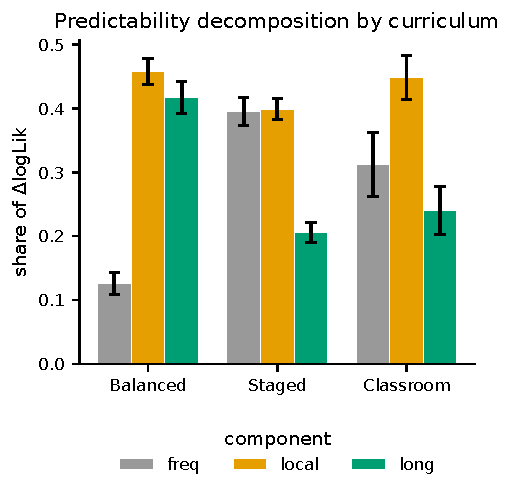
\includegraphics[width=\linewidth]{fig/interp/D5_decomp_shares.pdf}
        \caption{\textbf{D5 --- Predictability decomposition by curriculum.} Share of the MECO~L2 $\Delta\log L$ attributable to word log-frequency, local-context surprisal, and long-context surprisal, by curriculum (B1--B5, nld--eng). B1 draws more on word-frequency and local-context predictors than the staged curricula, which carry more share on long-context surprisal.}
        \label{fig:D5_decomp_shares}
    \end{subfigure}
    \hfill
    \begin{subfigure}[t]{0.48\linewidth}
        \centering
        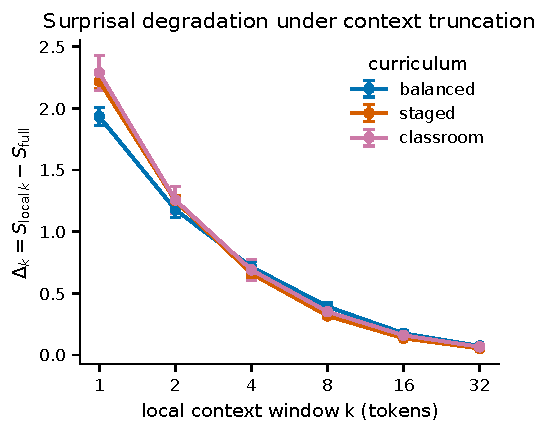
\includegraphics[width=\linewidth]{fig/interp/D6_context_degradation.pdf}
        \caption{\textbf{D6 --- Surprisal degradation under context truncation.} Surprisal degradation $\Delta_k = S_{\mathrm{local},k} - S_{\mathrm{full}}$ against context window $k$ (B1--B5, nld--eng); larger $\Delta_k$ at small $k$ indicates greater long-range reliance. On average, B1 degrades more than the staged curricula under aggressive truncation.}
        \label{fig:D6_context_degradation}
    \end{subfigure}

    \vspace{0.5em}

    % -------- Row 2 --------
    \begin{subfigure}[t]{0.48\linewidth}
        \centering
        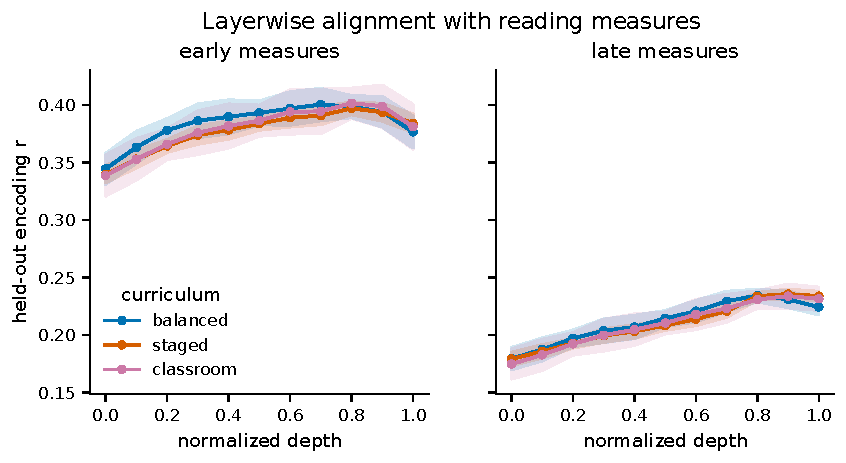
\includegraphics[width=\linewidth]{fig/interp/D8_layerwise_profile.pdf}
        \caption{\textbf{D8 --- Layerwise alignment with reading measures.} Predictive alignment (held-out encoding $r$) between layer activations and MECO~L2 reading-time measures against normalized depth ($0=$ embedding, $1=$ final layer), one panel per measure (first-pass / refixation / regression-in); colours = curriculum (B1 vs.\ B3-33, nld--eng FineWeb-100M). Higher $r$ indicates more reading-time variance explained at that depth.}
        \label{fig:D8_layerwise_profile}
    \end{subfigure}
    \hfill
    \begin{subfigure}[t]{0.48\linewidth}
        \centering
        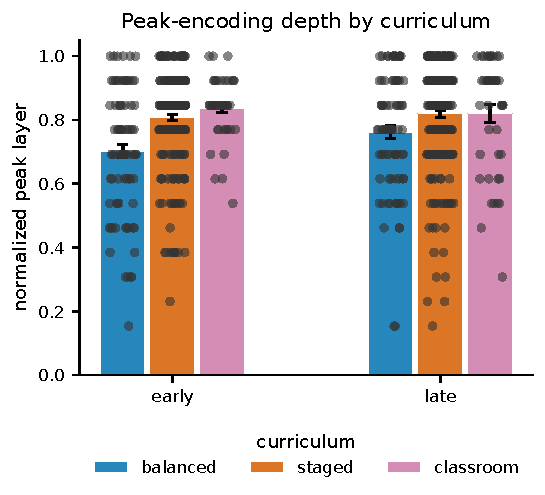
\includegraphics[width=\linewidth]{fig/interp/D9_peak_layer.pdf}
        \caption{\textbf{D9 --- Peak-encoding depth by curriculum.} Normalized depth ($0=$ embedding, $1=$ final layer) at which activations align most strongly with each MECO~L2 measure, by curriculum (B1--B5, nld--eng FineWeb-100M). B1 peaks deeper in the stack than the staged curricula, whose peak alignment is concentrated in mid-depth layers.}
        \label{fig:D9_peak_layer}
    \end{subfigure}

    \caption{Interpretability analyses across curricula showing decomposition of predictability, context dependence, layerwise alignment with reading measures, and peak encoding depth.}
    \label{fig:interp_grid}
\end{figure*}

\begin{figure}
    \centering
    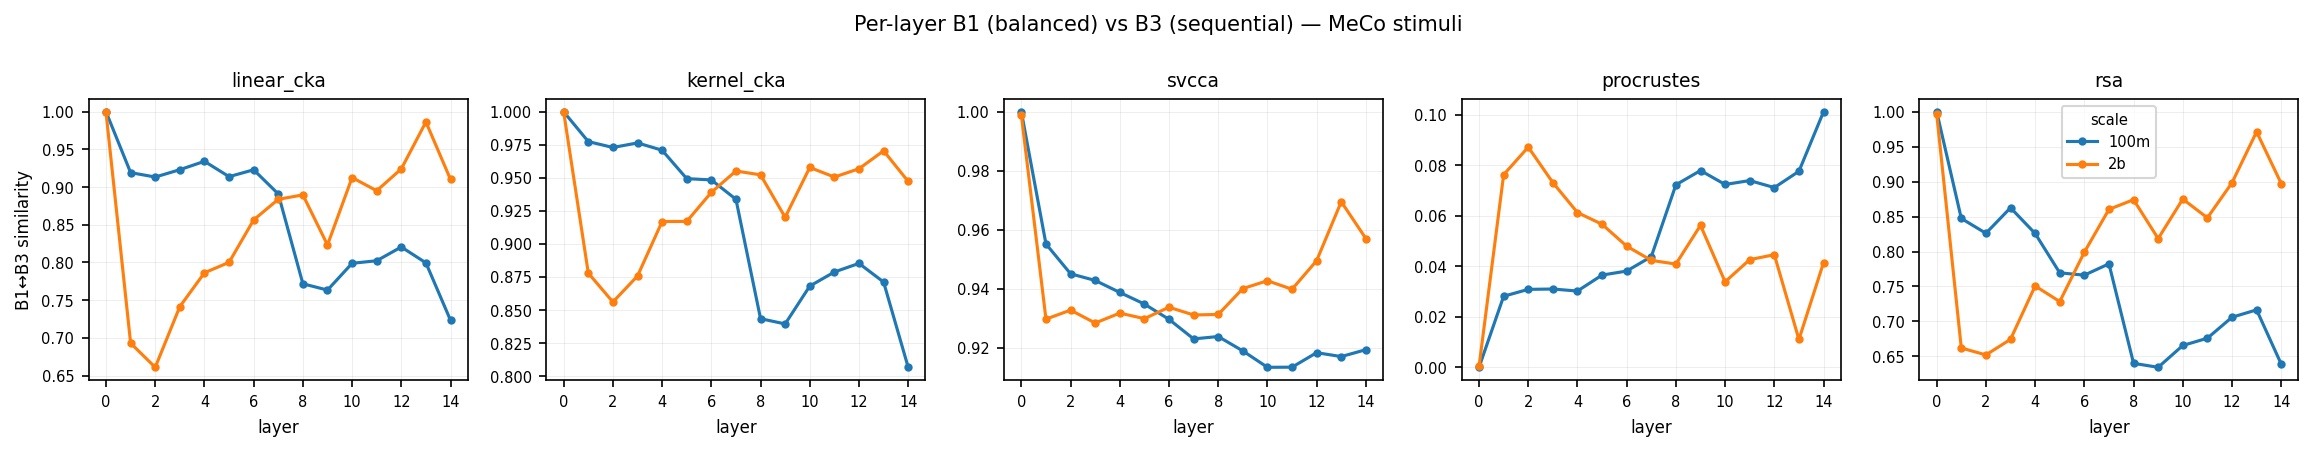
\includegraphics[width=1\linewidth]{fig/interp/repsim_b1_vs_b3.png}
    \caption{\textbf{Representational similarity, B1 vs.\ B3-33 (layer-wise).} CKA, RSA, Procrustes, and SVCCA similarity ($\in[0,1]$, $\uparrow$ more similar) between B1 and B3-33 nld--eng activations across layer index. Similarity stays near unity through embedding and early-block layers and drops at mid-to-late depth, where curriculum-induced divergence is concentrated, which overlaps with the layer band that shows the strongest MECO~L2 alignment (Fig.~\ref{fig:D8_layerwise_profile}).}
    \label{fig:repsim_b1_vs_b3}
\end{figure}



\paragraph{FLORES training dynamics.} The following figures track FLORES-200 surprisal over training; the catastrophic-forgetting framing is anchored to the per-language table in Block~C (Tab.~\ref{tab:flores_bi}).

\begin{figure}[!ht]
    \centering
    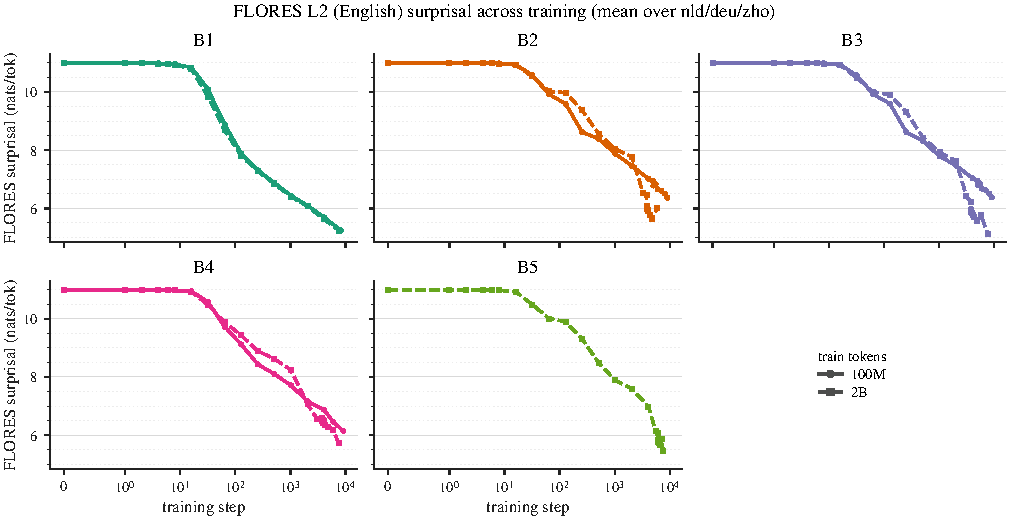
\includegraphics[width=1\linewidth]{fig/flores/fig_flores_main.pdf}
    \caption{\textbf{FLORES~L2 (English) surprisal across training.} Mean per-token FLORES-200 surprisal (nats/tok $=$ log-PPL; $\downarrow$ better) against training step (symlog), one panel per curriculum (B1--B5; sixth = legend), with 100M (solid) and 2B (dashed) cohorts overlaid, averaged over nld/deu/zho pairs. Staged-exposure curricula (B2/B3-33/B5) enter the B-GPT non-forgetting envelope earlier than B1 and remain inside it at convergence; we do not observe the legacy B-GPT \textsc{nl-en} sequential forgetting failure mode in any curriculum, under our evaluation definition of sequential forgetting (Tab.~\ref{tab:forgetting}).}
    \label{fig:flores_main}
\end{figure}


%\begin{figure}
%    \centering
%    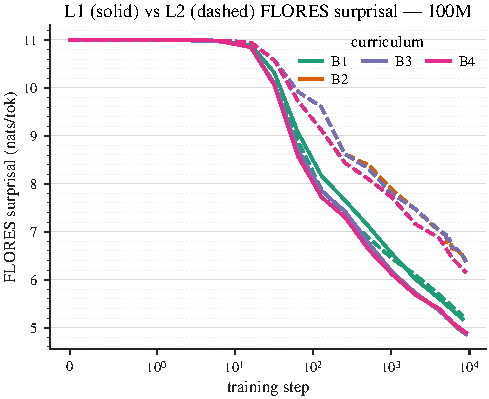
\includegraphics[width=1\linewidth]{fig/flores/fig_flores_l1l2.pdf}
%    \caption{\textbf{FLORES~L1 vs.\ L2 surprisal, per curriculum.} Mean per-token FLORES-200 surprisal (nats/tok) across training for L1 (solid) and L2 English (dashed), coloured by curriculum (B1--B5, nld--eng). Late-onset B5 retains lower L1 surprisal than B1 throughout training; all curricula reach comparable L2 English asymptotes.}
%    \label{fig:flores_l1l2}
%\end{figure}

\begin{figure}[!ht]
    \centering
    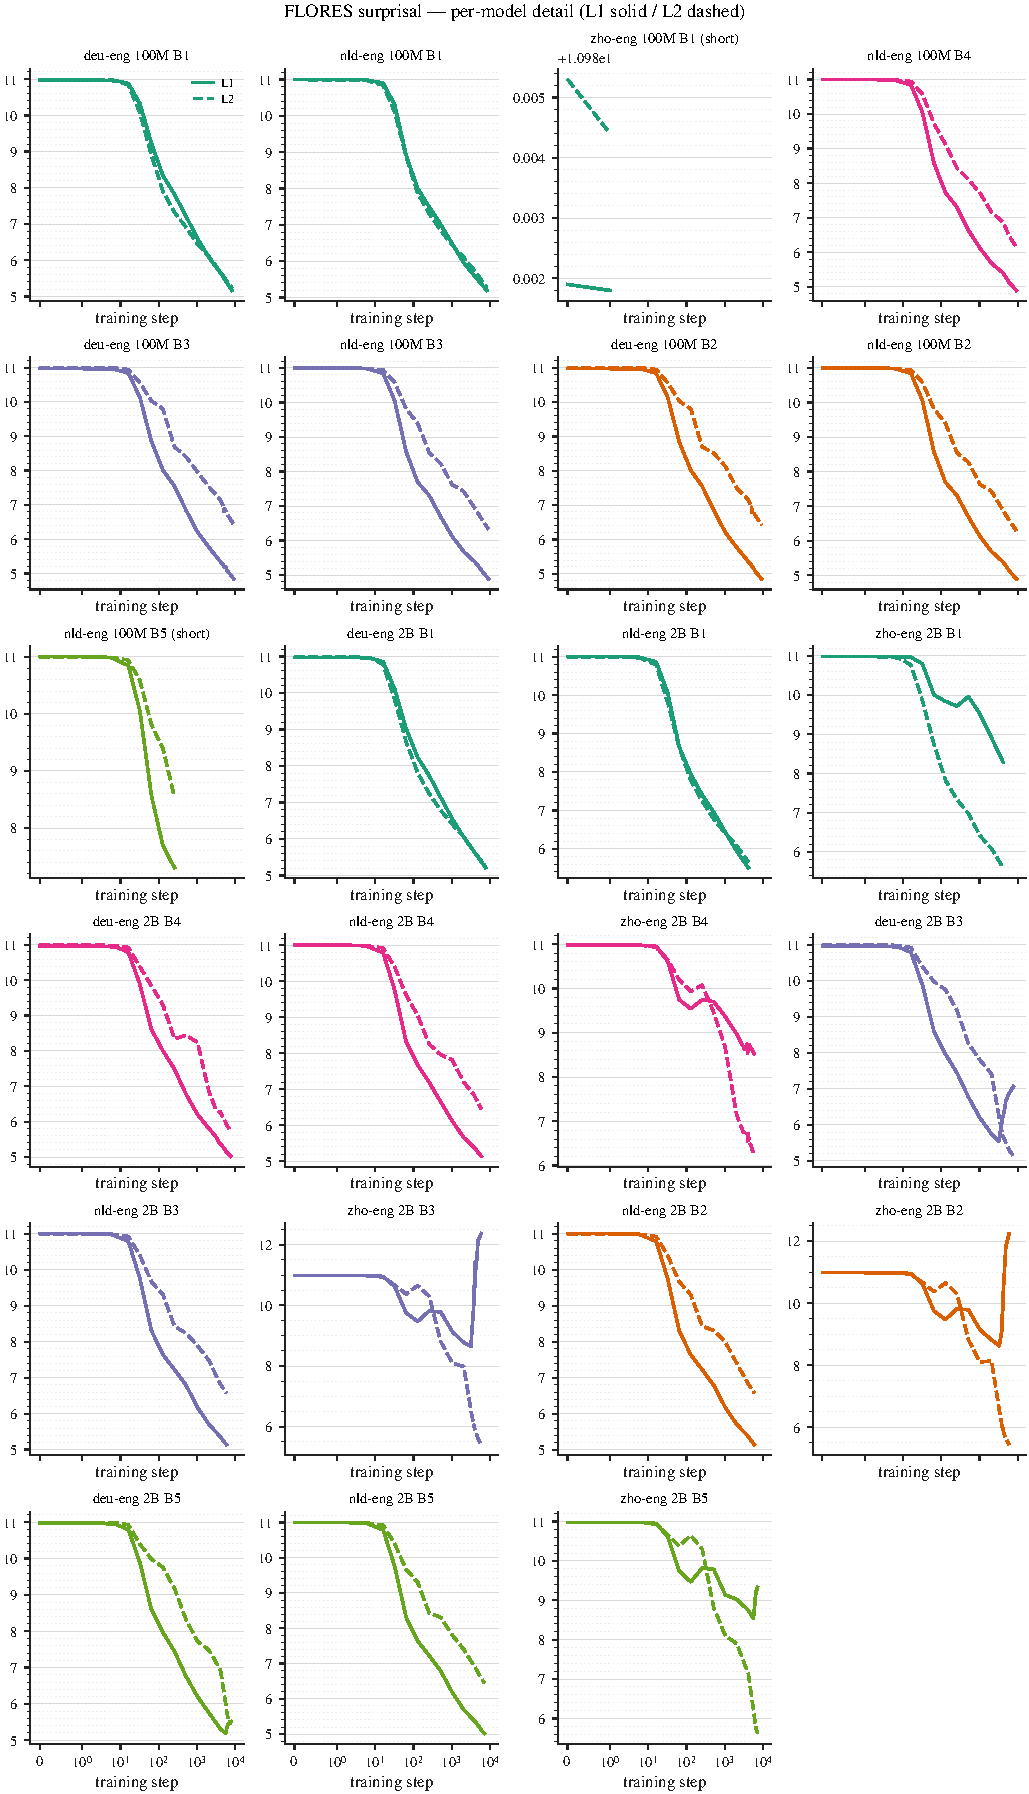
\includegraphics[width=1\linewidth]{fig/flores/appx_flores_per_model.pdf}
    \caption{\textbf{Per-model FLORES-200 surprisal across the full sweep.} Mean per-token FLORES-200 surprisal (nats/tok) for L1 and L2 English across every (L1, scale, curriculum) cell. Empty cells are untrained runs; the zho-100M-B1 cell is pending a retrain pass.}
    \label{fig:appx_flores_per_model}
\end{figure}

\newpage
\clearpage 

\subsection{Cross-model interpretability diagnostics}\label{sec:pico-cross-comp}

The Q1 and Q2 sweeps below constitute the cross-model interpretability diagnostics referenced from the body. Q1 identifies which interpretability metric varies most across L1 and across curriculum; Q2 reports how each metric co-varies with the downstream axes (BLiMP, MECO, BLiSS) over the same matched cohort.

\subsubsection{Q1 --- How does interpretability vary across models?}\label{sec:pico-q1}

\begin{figure}[!ht]
  \centering
  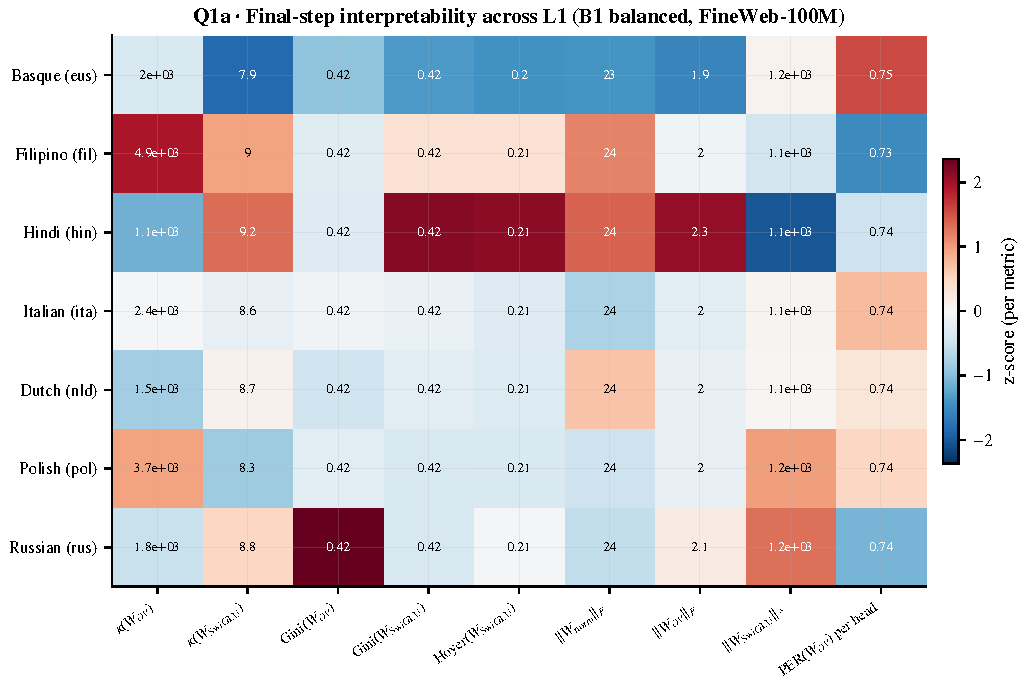
\includegraphics[width=\linewidth]{fig/pico_q1a_l1_heatmap.pdf}
  \caption{\textbf{Q1a -- L1 heatmap.} Final-step layer-mean of each \textsc{Pico-Analyze} metric against each L1 (B1 only); cell colour is the per-metric $z$-score, text is the raw value. $\kappa(W_{OV})$ shows the strongest variation across L1s in this sweep (Dutch $\sim\!1.5\!\times\!10^{3}$ to Hindi $\sim\!1.1\!\times\!10^{4}$); other metrics are nearly flat across L1. The OV-circuit spectral conditioning varies with typological distance from English more closely than the sparsity-style metrics do.}
  \label{fig:pico-q1a}
\end{figure}

\begin{figure}[!ht]
  \centering
  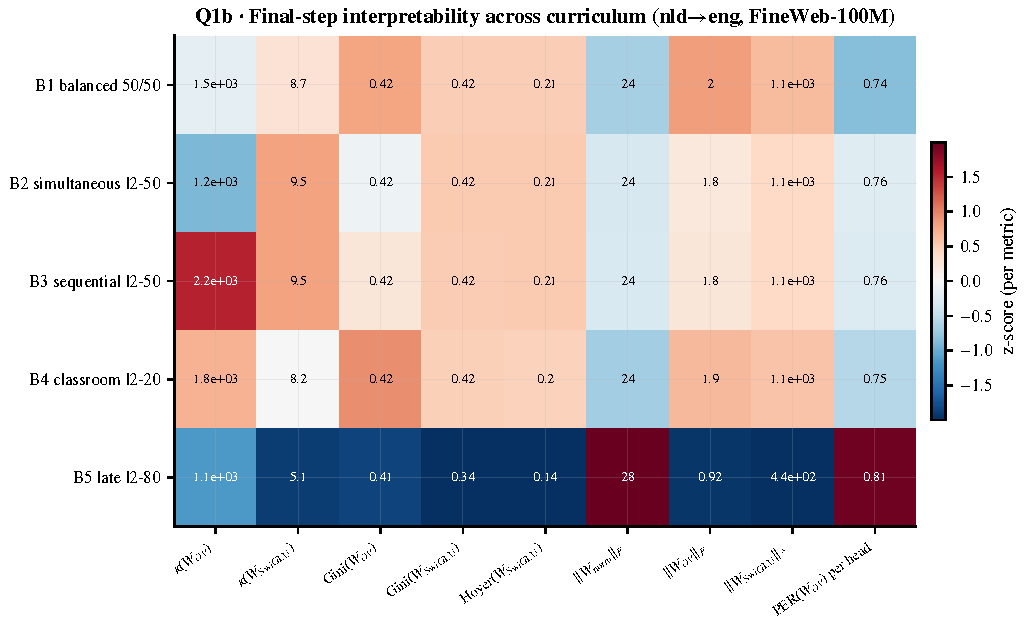
\includegraphics[width=\linewidth]{fig/pico_q1b_curriculum_heatmap.pdf}
  \caption{\textbf{Q1b -- Curriculum heatmap.} As Fig.~\ref{fig:pico-q1a}, over the nld--eng curriculum sweep (B1--B5). B5 (late L2) is an outlier on \texttt{gini-swiglu}, \texttt{hoyer-swiglu}, $\Vert W_{OV}\Vert_F$ and $\Vert W_{\text{SwiGLU}}\Vert_*$: less-sparse SwiGLU weights and a lower OV norm (0.92 vs.\ $\sim\!1.78$--$2.02$ for B1--B4). Delaying L2 exposure to 80\% of training co-occurs with an OV circuit that does not reach the high-norm, high-sparsity geometry of the other curricula.}
  \label{fig:pico-q1b}
\end{figure}

\begin{figure}[!ht]
  \centering
  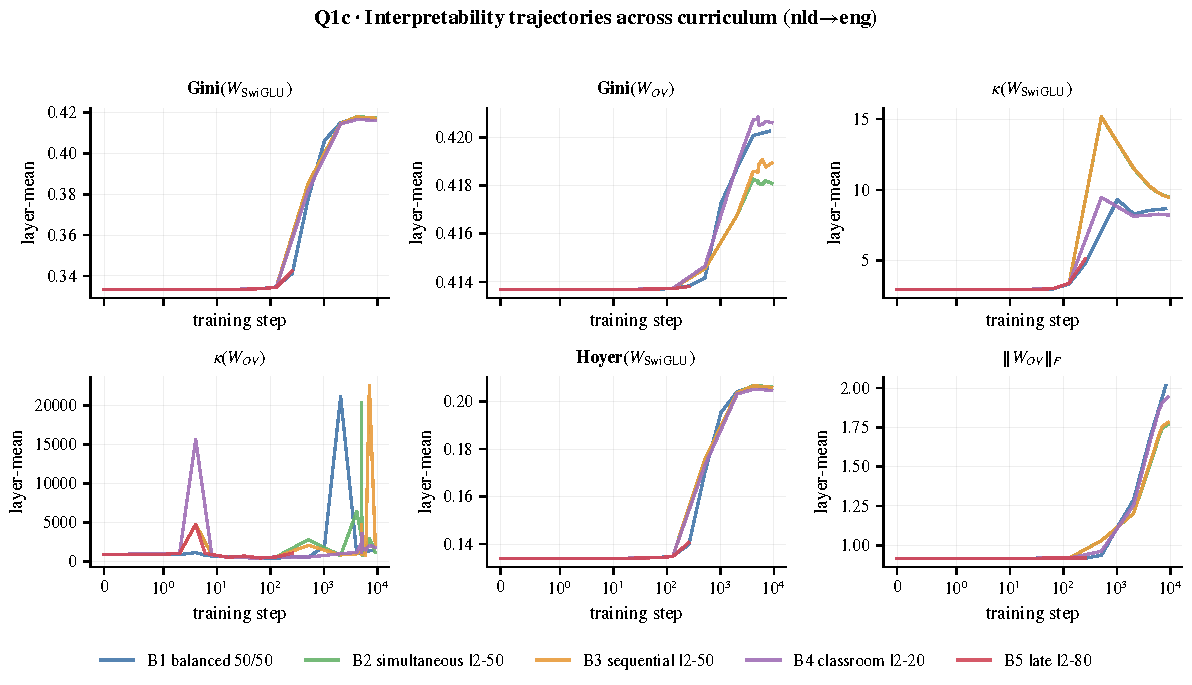
\includegraphics[width=\linewidth]{fig/pico_q1c_curriculum_trajectories.pdf}
  \caption{\textbf{Q1c -- Curriculum trajectories.} Layer-mean trajectories across training for B1--B5 (nld--eng) on six representative metrics. All emerge between step 256 and 1024 and saturate by 8k; B5 follows the same shape at a lower plateau, i.e.\ the curriculum difference is in plateau height rather than onset timing.}
  \label{fig:pico-q1c}
\end{figure}

\begin{figure}[!ht]
  \centering
  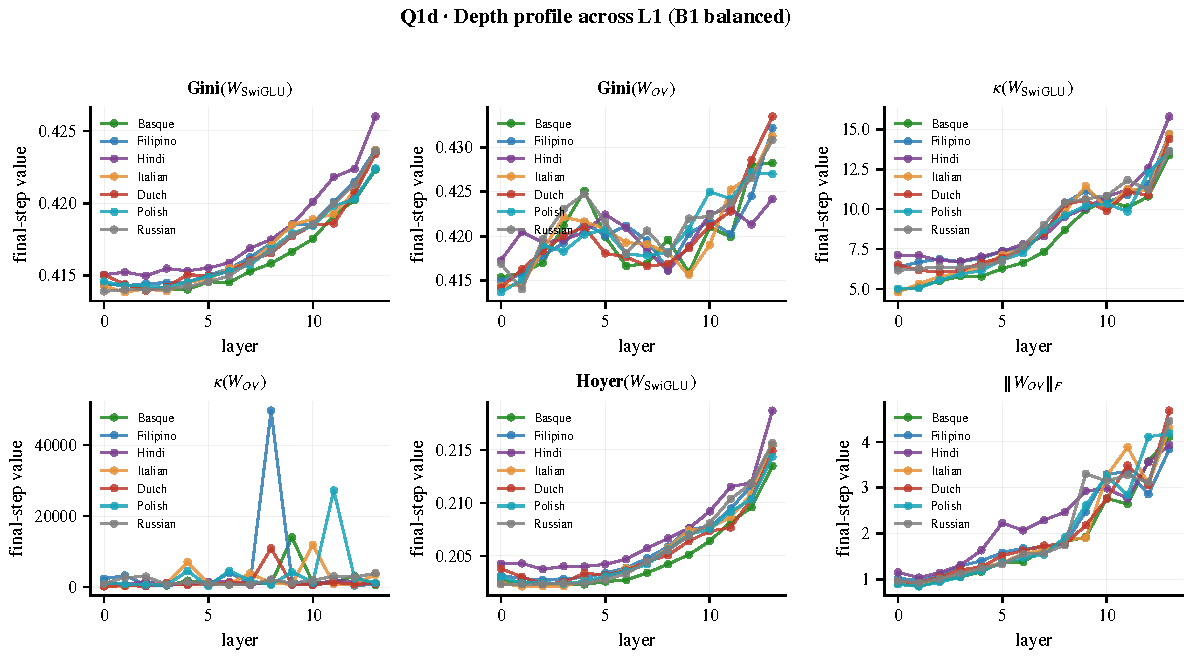
\includegraphics[width=\linewidth]{fig/pico_q1d_depth_profile_l1.pdf}
  \caption{\textbf{Q1d -- Depth profile across L1.} Final-step value against layer index, one panel per metric, lines = L1 (B1 only). The OV-circuit signal is concentrated in mid-to-late layers; sparsity metrics (Gini, Hoyer) are layer-flat. With Fig.~\ref{fig:pico-q1a}, the cross-L1 variation is concentrated in the same depth band as the OV induction circuitry.}
  \label{fig:pico-q1d}
\end{figure}

\begin{figure}[!ht]
  \centering
  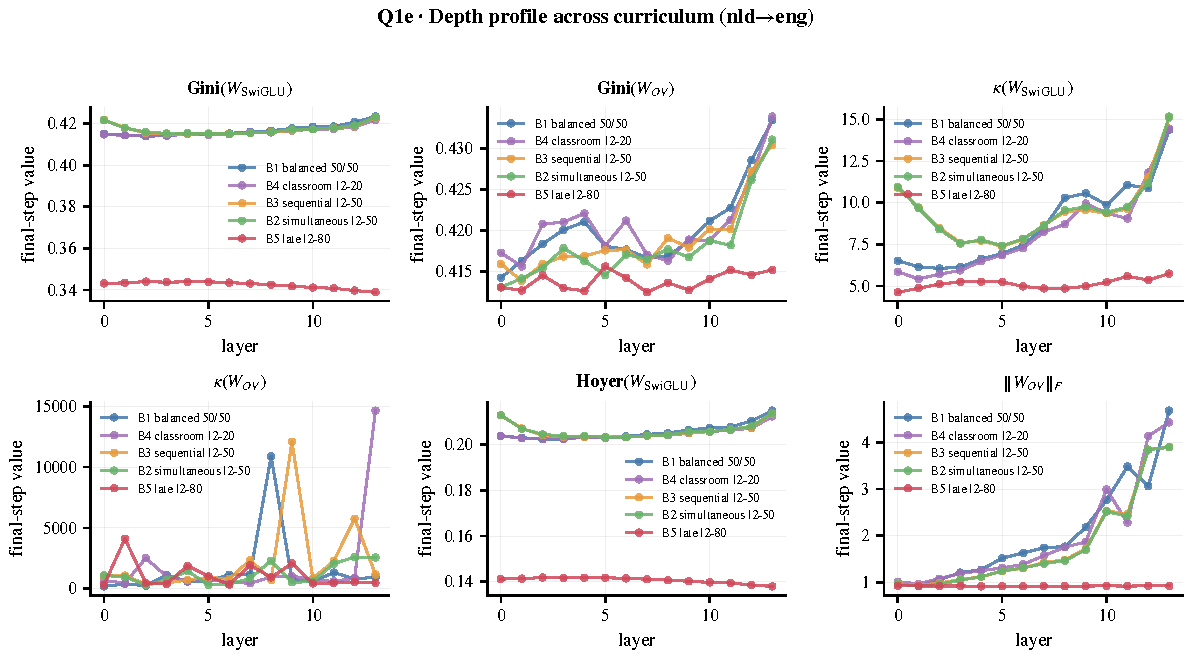
\includegraphics[width=\linewidth]{fig/pico_q1e_depth_profile_curriculum.pdf}
  \caption{\textbf{Q1e -- Depth profile across curriculum.} As Fig.~\ref{fig:pico-q1d}, lines = curriculum (B1--B5, nld--eng). The B5-vs-B1--B4 plateau gap of Fig.~\ref{fig:pico-q1c} falls within the mid-to-late layers that host the OV induction band.}
  \label{fig:pico-q1e}
\end{figure}

\subsubsection{Q2 --- Do interpretability metrics correlate with downstream behaviour?}\label{sec:pico-q2}

\paragraph{Statistical scope.} All Q2 results below are exploratory. Each correlation is computed over $n=5$ curriculum points on highly correlated curricula; no significance testing, permutation test, or confidence interval is reported. The $r$-values are intended as hypothesis-generating, not as estimates of a population effect, and should not be read as evidence of causal relationships.

\begin{figure}[!ht]
  \centering
  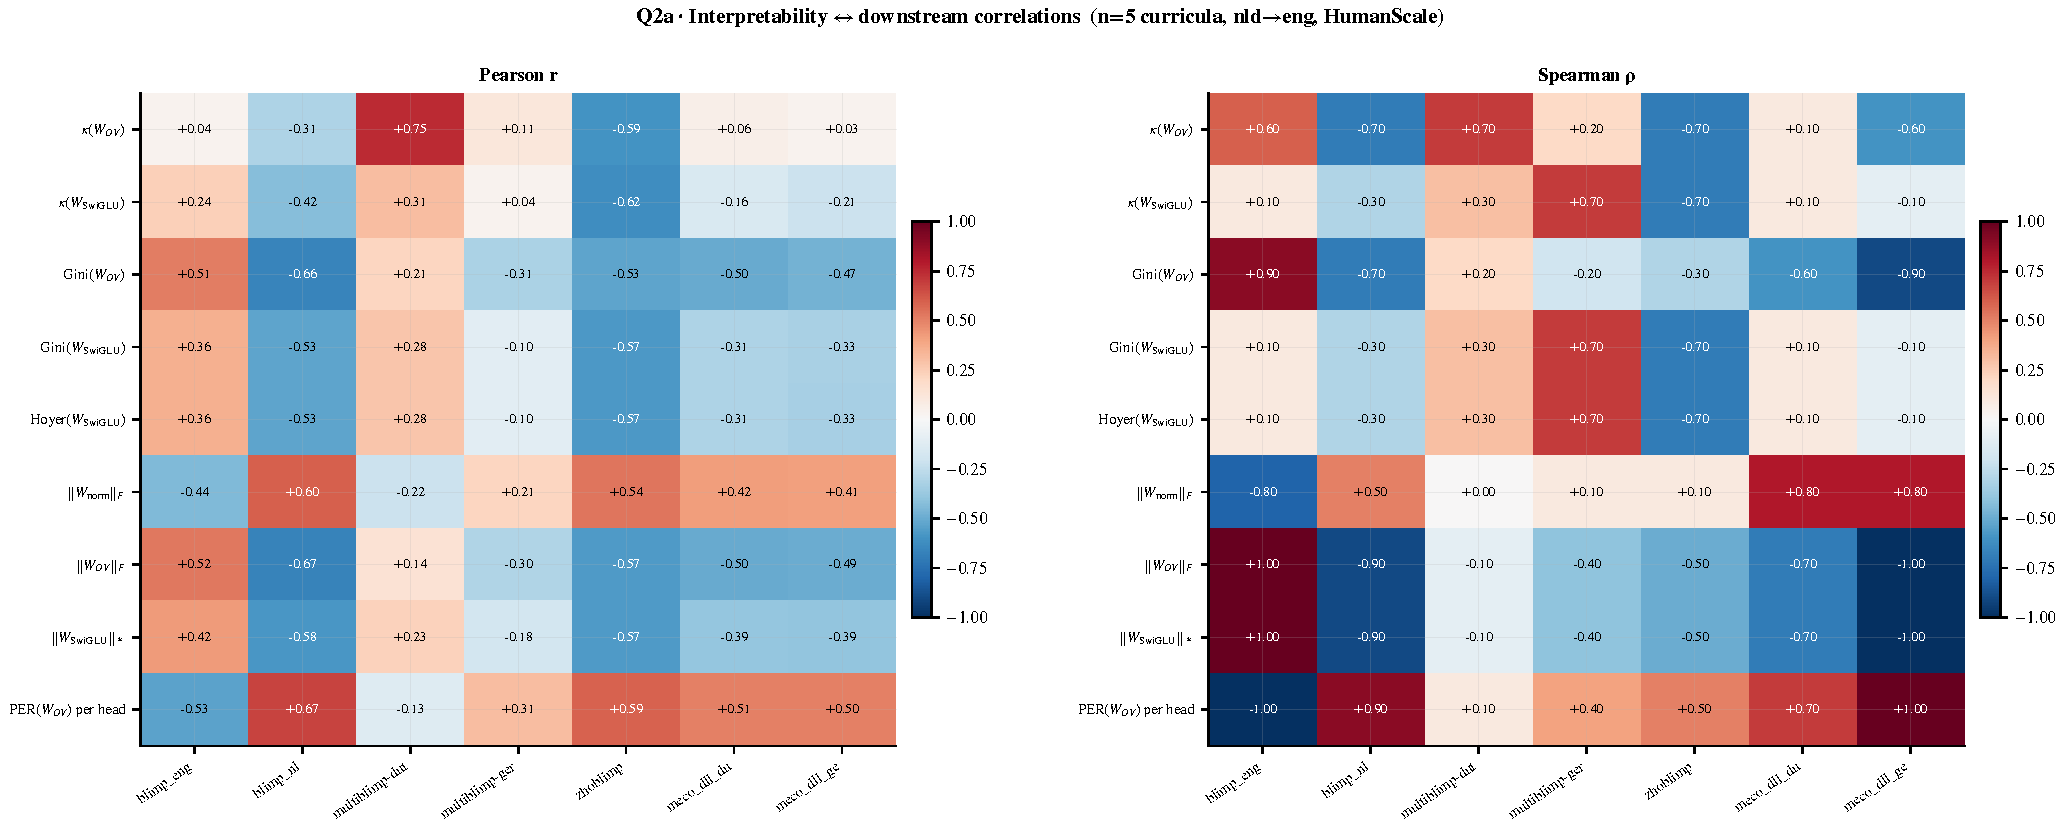
\includegraphics[width=\linewidth]{fig/pico_q2a_corr_heatmap.pdf}
  \caption{\textbf{Q2a -- Correlation heatmap.} Pearson $r$ and Spearman $\rho$ for each (interpretability $\times$ downstream) pair across the nld--eng sweep ($n=5$, exploratory). The pattern is asymmetric: OV+SwiGLU sparsity/norm metrics correlate positively with L2 English BLiMP and negatively with L1-side BLiMP and human-RT alignment. $\Vert W_{\text{norm}}\Vert_F$ is the only metric correlating positively with both Dutch BLiMP and MECO surprisal-fit. $\kappa(W_{OV})$ is uninformative on this sweep ($|r|\le 0.31$) despite showing the strongest cross-L1 variation in Q1a.}
  \label{fig:pico-q2a}
\end{figure}

\begin{figure}[!ht]
  \centering
  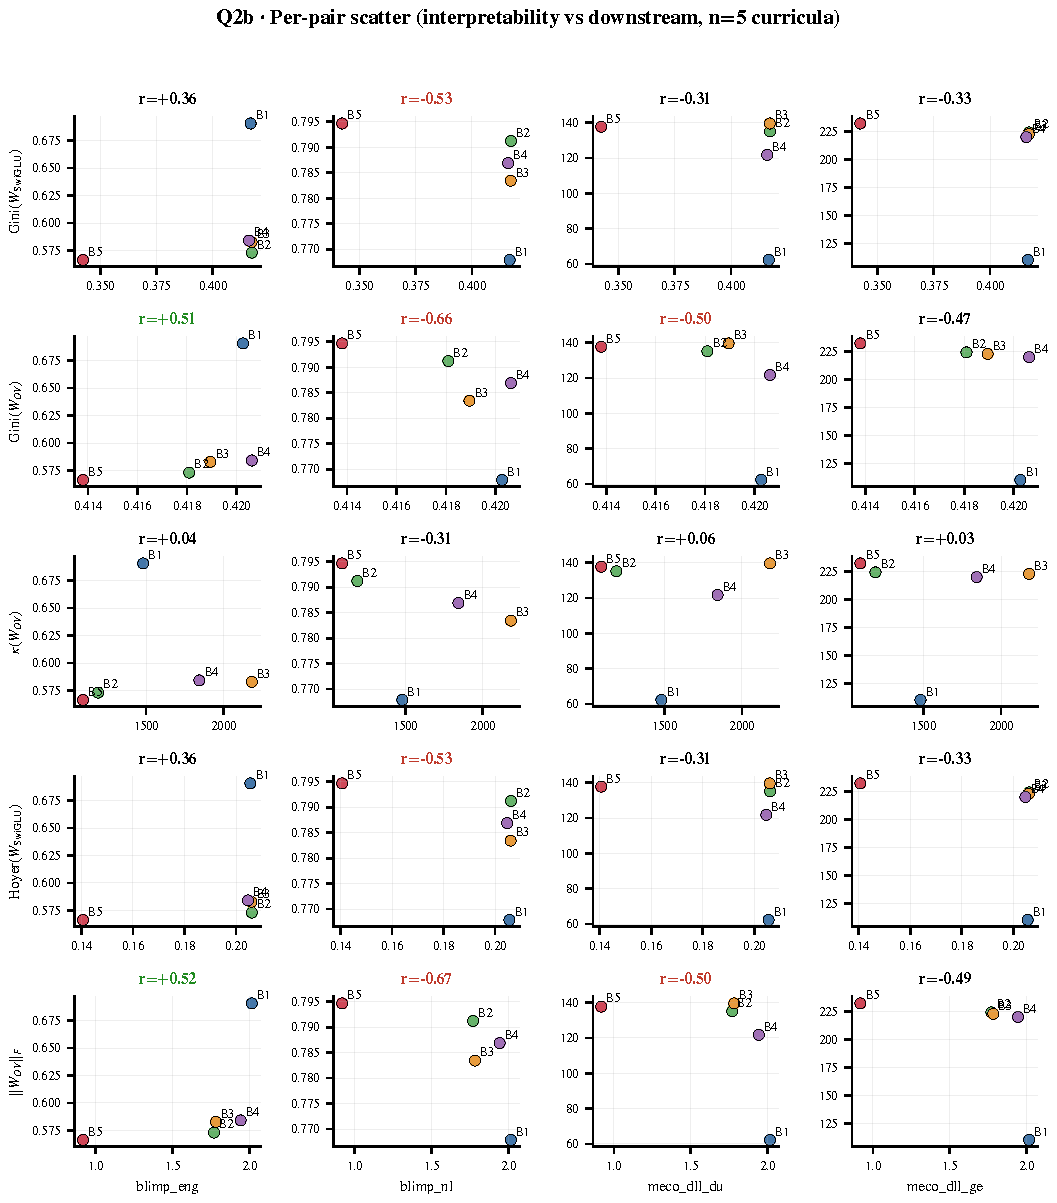
\includegraphics[width=\linewidth]{fig/pico_q2b_scatter_grid.pdf}
  \caption{\textbf{Q2b -- Per-pair scatter.} Scatter for a curated subset of (interpretability $\times$ downstream) pairs over the $n=5$ nld--eng curricula; curriculum labels annotated, per-panel Pearson $r$ in the title. The B1$\leftrightarrow$B5 separation along $\Vert W_{OV}\Vert_F$ and Gini$(W_{\text{SwiGLU}})$ is visible in the point cloud; trend estimates are exploratory given $n=5$.}
  \label{fig:pico-q2b}
\end{figure}

\begin{figure}[!ht]
  \centering
  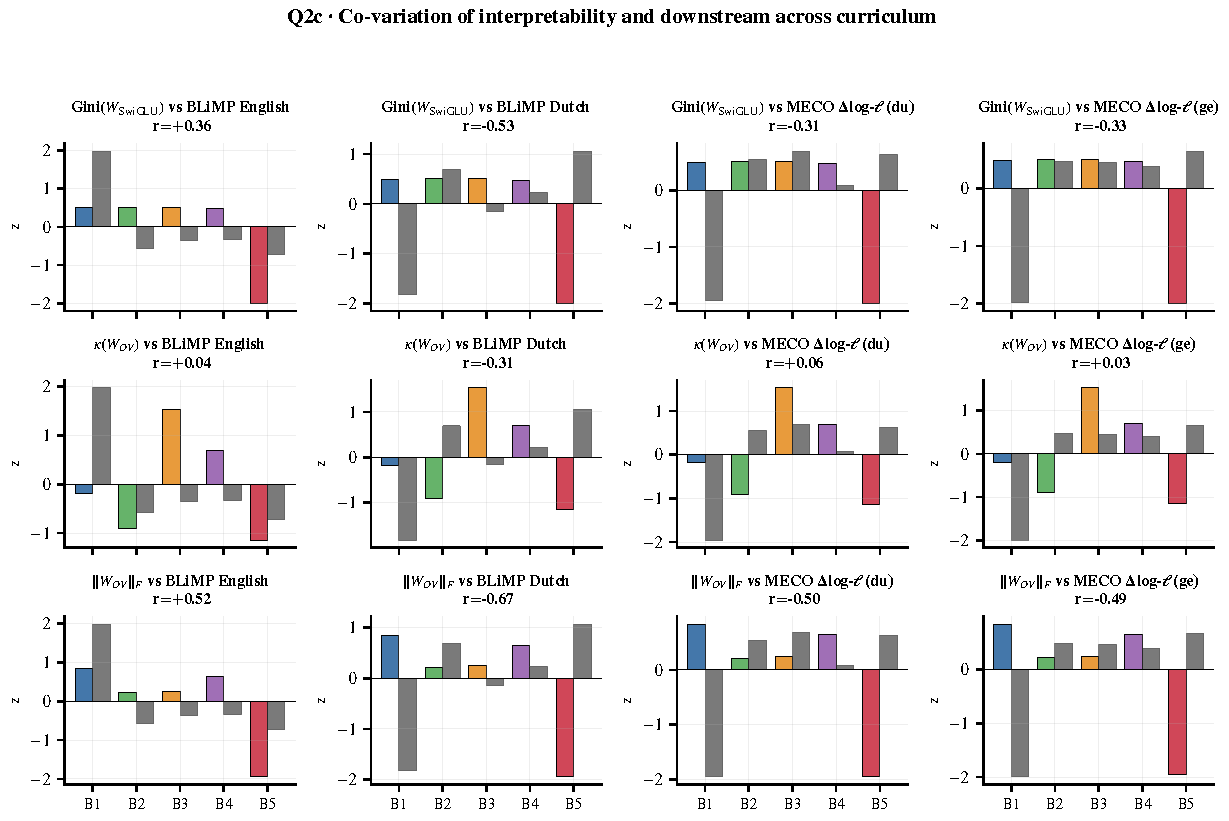
\includegraphics[width=\linewidth]{fig/pico_q2c_paired_bars.pdf}
  \caption{\textbf{Q2c -- Paired $z$-scored bars.} Per curriculum (B1--B5), each interpretability metric paired with a downstream metric on a common $z$-axis (same height $\Rightarrow$ same direction). Sign-flip clusters (e.g.\ $\Vert W_{OV}\Vert_F$ vs.\ BLiMP-nl; Gini$(W_{\text{SwiGLU}})$ vs.\ MECO~du) show the specialisation--generalisation pattern of \S\ref{sec:pico-cross-comp}.}
  \label{fig:pico-q2c}
\end{figure}

\subsubsection{Principal correlations and summary}\label{sec:pico-headline}

The principal Q2 results reproduce the per-pair Pearson $r$ values plotted in Fig.~\ref{fig:pico-q2a} (full table in the released \texttt{ledger\_q2\_joined.csv}); selected pairs are in Table~\ref{tab:pico-q2-headline}.

\begin{table}[h]
  \centering
  \small
  \caption{Pearson $r$ across the $n=5$ nld--eng curriculum sweep (B1--B5) for selected (interpretability, downstream) pairs. Bold cells exceed $|r|>0.5$. No multiple-comparison correction is applied. Exploratory; see statistical-scope note in \S\ref{sec:pico-q2}.}
  \label{tab:pico-q2-headline}
  \begin{tabular}{lrrrr}
    \toprule
    metric & BLiMP-eng & BLiMP-nl & MECO-du & MECO-ge \\
    \midrule
    $\Vert W_{OV}\Vert_F$       & \textbf{+0.52} & \textbf{$-$0.67} & $-$0.50 & $-$0.49 \\
    Gini$(W_{\text{SwiGLU}})$   & $+$0.36        & \textbf{$-$0.53} & $-$0.31 & $-$0.33 \\
    Hoyer$(W_{\text{SwiGLU}})$  & $+$0.36        & \textbf{$-$0.53} & $-$0.37 & $-$0.33 \\
    $\Vert W_{\text{norm}}\Vert_F$ & $-$0.44     & \textbf{$+$0.60} & \textbf{$+$0.54} & $+$0.42 \\
    $\kappa(W_{OV})$            & $+$0.04        & $-$0.31          & $+$0.06 & $+$0.03 \\
    \bottomrule
  \end{tabular}
\end{table}

These metrics are more consistent with a decomposition into partially independent axes than with a single scalar quality dimension. On this sweep, higher Gini/Hoyer/Frobenius on the OV+SwiGLU subspaces co-occurs with higher BLiMP-eng and with lower L1 transfer and psycholinguistic alignment. The curriculum with the highest BLiMP-eng (B1, balanced) and the one with the highest L1 retention and human-RT alignment (B5, late L2) fall at opposite ends of this ordering. However, these are exploratory associations; we leave more thorough investigation of these conditions to future work. 

%\paragraph{Caveats.} (i) $n=5$ per correlation; $r$-values exploratory; bootstrap CIs pending. (ii) Downstream evaluations are at \textsc{HumanScale}; interpretability metrics at \textsc{FineWeb}-100M (same parameter count and token budget, different corpora) --- a matched-corpus re-run would tighten the join. (iii) \textsc{BLiSS} excluded as noted above. (iv) The \texttt{rus-eng} \textsc{Pico} run contributes to Q1 only.


\newpage
\clearpage 

\section{Detailed Downstream Results}\label{sec:downstream}

We report \beetle \textsc{MultiBLiMP} per-language accuracy (Tab.~\ref{tab:multiblimp}), \textsc{FLORES-200} PPL split into monolingual anchors (Tab.~\ref{tab:flores_mono}) and bilingual conditions (Tab.~\ref{tab:flores_bi}), and catastrophic forgetting by acquisition schedule (Tab.~\ref{tab:forgetting}). All \textsc{FLORES-200} metrics are reported either as per-token negative log-likelihood (nats/tok, equivalently log-PPL) or as perplexity; lower is better unless otherwise noted. B3-33 nld--eng reaches the best \textsc{Beetle} Dutch grammaticality (90.3\%), and the structured-exposure advantage attenuates across the typological-distance gradient (Dutch~$>$~German~$>$~French~$>$~Persian~$>$~Bulgarian). On FLORES-200, B1 balanced and B2 simultaneous incur the smallest L1 PPL penalty after L2 introduction. \label{appcomp:phase}

\begin{table}[!ht]
  \centering
  \small
  \caption{\textsc{MultiBLiMP} accuracy (\%) across five languages for nld--eng \textsc{HumanScale} \beetle{} models and baselines. Bold marks the best per-column result.}
  \label{tab:multiblimp}
  \begin{tabular}{lrrrrr}
    \toprule
    Condition & Dutch & German & French & Persian & Bulgarian \\
    \midrule
    \multicolumn{6}{l}{\emph{Monolingual anchors}} \\
    mono-ENG & 53.0 & 60.3 & 60.8 & 52.9 & 63.5 \\
    mono-NLD & 88.9 & 67.4 & 58.9 & 40.4 & 62.4 \\
    \midrule
    \multicolumn{6}{l}{\emph{\beetle{} curricula}} \\
    B1       & 87.6 & 67.6 & 61.5 & 53.4 & 62.5 \\
    B2       & 88.8 & 73.3 & 63.3 & 49.5 & 62.4 \\
    B3-33    & \textbf{90.3} & 72.9 & 62.0 & 51.4 & 62.3 \\
    B3-0     & 89.7 & 70.9 & 61.8 & 51.3 & 62.6 \\
    B4       & 89.8 & 72.3 & 61.5 & 51.6 & 62.3 \\
    B5       & 88.5 & 72.1 & 62.2 & 51.2 & 62.0 \\
    \midrule
    \multicolumn{6}{l}{\emph{Continual-learning baselines}} \\
    episodic & 86.4 & 70.7 & 61.7 & 54.7 & 61.2 \\
    ewc      & 88.8 & 73.3 & 63.3 & 49.5 & 62.4 \\
    lamol    & 88.8 & 73.3 & 63.3 & 49.5 & 62.4 \\
    \midrule
    \multicolumn{6}{l}{\emph{BLOOM ladder}} \\
    BLOOM-560m & 59.1 & 65.8 & 81.4 & 55.5 & 58.8 \\
    BLOOM-1b1  & 62.8 & 76.5 & 94.0 & 55.6 & 64.3 \\
    BLOOM-1b7  & 65.9 & 75.8 & 93.1 & 57.9 & 64.7 \\
    BLOOM-3b   & 65.6 & 80.6 & \textbf{97.9} & 59.9 & 63.9 \\
    BLOOM-7b1  & 64.6 & \textbf{82.7} & 95.3 & \textbf{60.1} & \textbf{67.2} \\
    \bottomrule
  \end{tabular}
\end{table}

\begin{table}[t]
  \centering
  \small
  \caption{\textsc{FLORES-200} monolingual anchors: per-sentence perplexity (PPL, $\downarrow$ better). These rows are the per-language reference against which the bilingual $\Delta$-NLL of Tab.~\ref{tab:flores_bi} is computed.}
  \label{tab:flores_mono}
  \begin{tabular}{lrrrr}
    \toprule
    Anchor & NLD & ENG & DEU & ZHO \\
    \midrule
    mono-ENG & ---  & 781 & ---  & ---  \\
    mono-NLD & 324  & --- & ---  & ---  \\
    mono-DEU & ---  & --- & 400  & ---  \\
    mono-ZHO & ---  & --- & ---  & 3839 \\
    \bottomrule
  \end{tabular}
\end{table}

\begin{table}[!ht]
  \centering
  \small
  \caption{\textsc{FLORES-200} bilingual conditions: per-sentence PPL and $\Delta$-NLL relative to the matched monolingual anchor of Tab.~\ref{tab:flores_mono} (negative = lower PPL than monolingual). Bold marks minimum PPL / $\Delta$-NLL closest to zero per language. HS $=$ \textsc{HumanScale}; FW $=$ \textsc{FineWeb}.}
  \label{tab:flores_bi}
  \begin{tabular}{lrrrr}
    \toprule
    Condition & NLD PPL & NLD $\Delta$ & ENG PPL & ENG $\Delta$ \\
    \midrule
    B1 nld-eng HS  & 318 & +0.02   & 412 & $-$0.57 \\
    B1 nld-eng FW  & 81  & $-$1.28 & 109 & $-$1.84 \\
    B2 nld-eng FW  & \textbf{75} & $-$1.40 & 303 & $-$0.87 \\
    B2 eng-nld FW  & 273 & $-$0.08 & \textbf{94} & $-$2.01 \\
    B3-33 nld-eng HS & 268 & $-$0.22 & 1033 & +0.24 \\
    B5 nld-eng HS  & 268 & $-$0.23 & 987 & +0.22 \\
    BLOOM-1b1      & 402 & +0.23   & 122 & $-$1.78 \\
    BLOOM-560m     & 7888 & +2.43  & 7625 & +0.33 \\
    \midrule
    \multicolumn{5}{l}{\emph{DEU / ZHO cells (separate anchors):}} \\
    B1 eng-deu FW  & \multicolumn{2}{l}{DEU PPL \textbf{81} ($-$1.44)} & 104 & $-$1.87 \\
    B3-33 zho-eng HS & \multicolumn{2}{l}{ZHO PPL 7223 (+0.36)} & 1277 & +0.50 \\
    \bottomrule
  \end{tabular}
\end{table}

\paragraph{Catastrophic forgetting.} Absolute values in Tab.~\ref{tab:forgetting} should not be compared across schedules, which differ in trajectory length and evaluation coverage; only within-schedule ordering is intended to be read. We do not observe evidence of the legacy B-GPT \textsc{nl-en} sequential forgetting failure mode in any \beetle{} curriculum.

\begin{table}[!ht]
  \centering
  \small
  \caption{Catastrophic forgetting aggregated by acquisition schedule and L1, sorted by \% sentences worse (ascending) so that the best-retention cells appear first. Mean $\Delta$-PPL: mean per-sentence PPL increase over the matched monolingual baseline. CF Log-Ratio: mean log perplexity ratio (positive = worse). $N$ = number of (model, L2-language) cells. Absolute magnitudes are not comparable across schedules (see text); only within-schedule ordering is meaningful.}
  \label{tab:forgetting}
  \begin{tabular}{llrrrr}
    \toprule
    L1 & Schedule & Mean $\Delta$-PPL & CF Log-Ratio & \% Worse & $N$ \\
    \midrule
    German  & Balanced     & \textbf{157} & \textbf{+0.14} & \textbf{57} & 2 \\
    German  & Sequential   & 286   & +0.34 & 59  & 2 \\
    German  & Part-time    & 396   & +0.48 & 66  & 3 \\
    German  & Heritage     & 2418  & +0.76 & 67  & 6 \\
    German  & Simultaneous & 1111  & +0.61 & 68  & 4 \\
    German  & Late L2      & 118823 & +3.14 & 93 & 4 \\
    Chinese & Simultaneous & 676   & +2.90 & 100 & 1 \\
    Dutch   & Heritage     & 371   & +2.48 & 100 & 2 \\
    Dutch   & Simultaneous & 774   & +3.17 & 100 & 3 \\
    Dutch   & Balanced     & 1048  & +3.24 & 100 & 8 \\
    Chinese & Late L2      & 1445  & +3.63 & 100 & 5 \\
    Chinese & Heritage     & 1498  & +3.63 & 100 & 4 \\
    Chinese & Balanced     & 7350  & +4.42 & 100 & 9 \\
    Dutch   & Late L2      & 35979 & +4.86 & 100 & 2 \\
    Dutch   & Part-time    & 36071 & +5.14 & 100 & 2 \\
    Chinese & Part-time    & 30567 & +6.65 & 100 & 1 \\
    Dutch   & Sequential   & 71758 & +7.66 & 100 & 1 \\
    \bottomrule
  \end{tabular}
\end{table}

%\paragraph{Full-resolution main-body reproductions.} High-resolution reproductions of the main-body figures (the MultiBLiMP Pareto and token-efficiency panels, the MECO~L2 curriculum and token-efficiency panels, the FLORES-vs-B-GPT comparison, and the per-participant MECO~L2 $\Delta\log L$ heatmap) are provided with the released artefacts rather than reprinted here, since they introduce no analysis axis beyond their main-body counterparts. The per-participant MECO~L2 heatmap (participant $\times$ model) is the one item in this group with appendix-only detail and is retained in the release as \texttt{fig\_meco\_l2\_participants\_heatmap.pdf}.

\clearpage 
\newpage 

\section{Supplementary BLiSS and Pedagogical Results and Ablations}\label{sec:supp-results}

We provide detailed supplementary results of \beetle BLiSS performance in \autoref{appcomp:bliss} and downstream pedagogical evaluations in \autoref{appcomp:peda}. 

\subsection{BLiSS supplementary results}\label{appcomp:bliss}

The load-bearing BLiSS result for the curriculum trade-off is the final-checkpoint relationship between BLiSS NGS and MECO~L2 $\Delta\log L$ (Fig.~\ref{fig:bliss_vs_meco}): the curriculum ordering on BLiSS NGS runs in the opposite direction of the MECO~L2 ordering of \S\ref{sec:pareto}. 

%The supporting views --- best-cell-vs-baseline, the \textsc{FineWeb}~2B curriculum frontier, the CPS / RP$@\tau$ diagnostics, the aggregated-by-L1 NGS, and the NGS/CPS/RP$@\tau$ trade-off --- are released as artefacts (\texttt{fig\_bliss\_*.pdf}); each restates the same ordering on a different BLiSS sub-metric.

\begin{figure}[!ht]
  \centering
  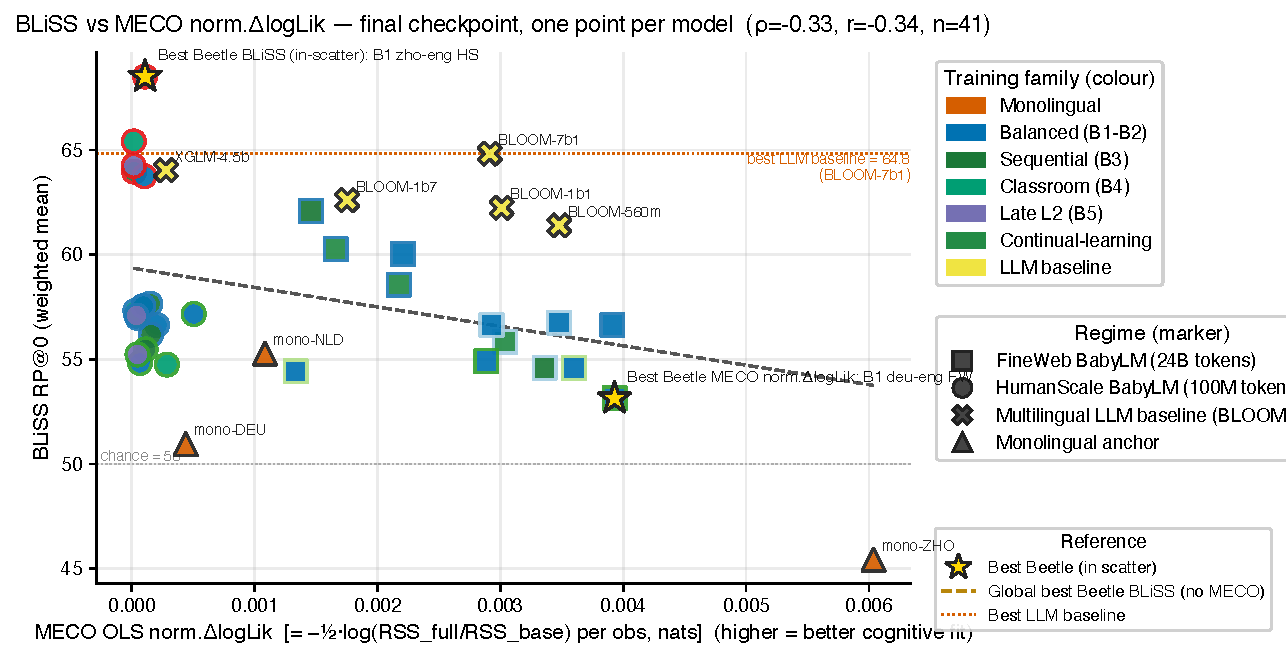
\includegraphics[width=\linewidth]{fig/fig_bliss_vs_meco_final.pdf}
  \caption{\textbf{BLiSS NGS vs.\ MECO~L2 $\Delta\log L$ (final checkpoint).} Per-curriculum final-checkpoint scatter, coloured by curriculum. The curriculum ordering on BLiSS NGS runs in the opposite direction of the MECO~L2 ordering of \S\ref{sec:pareto}.}
  \label{fig:bliss_vs_meco}
\end{figure}

\clearpage 
\newpage 

\section{BGPT v \beetle{} Comparison on Structural Priming} \label{bgpt-beetle-priming-comparison}

\subsection{Effect of Exposure Curricula on Priming}



\begin{figure}
    \centering
    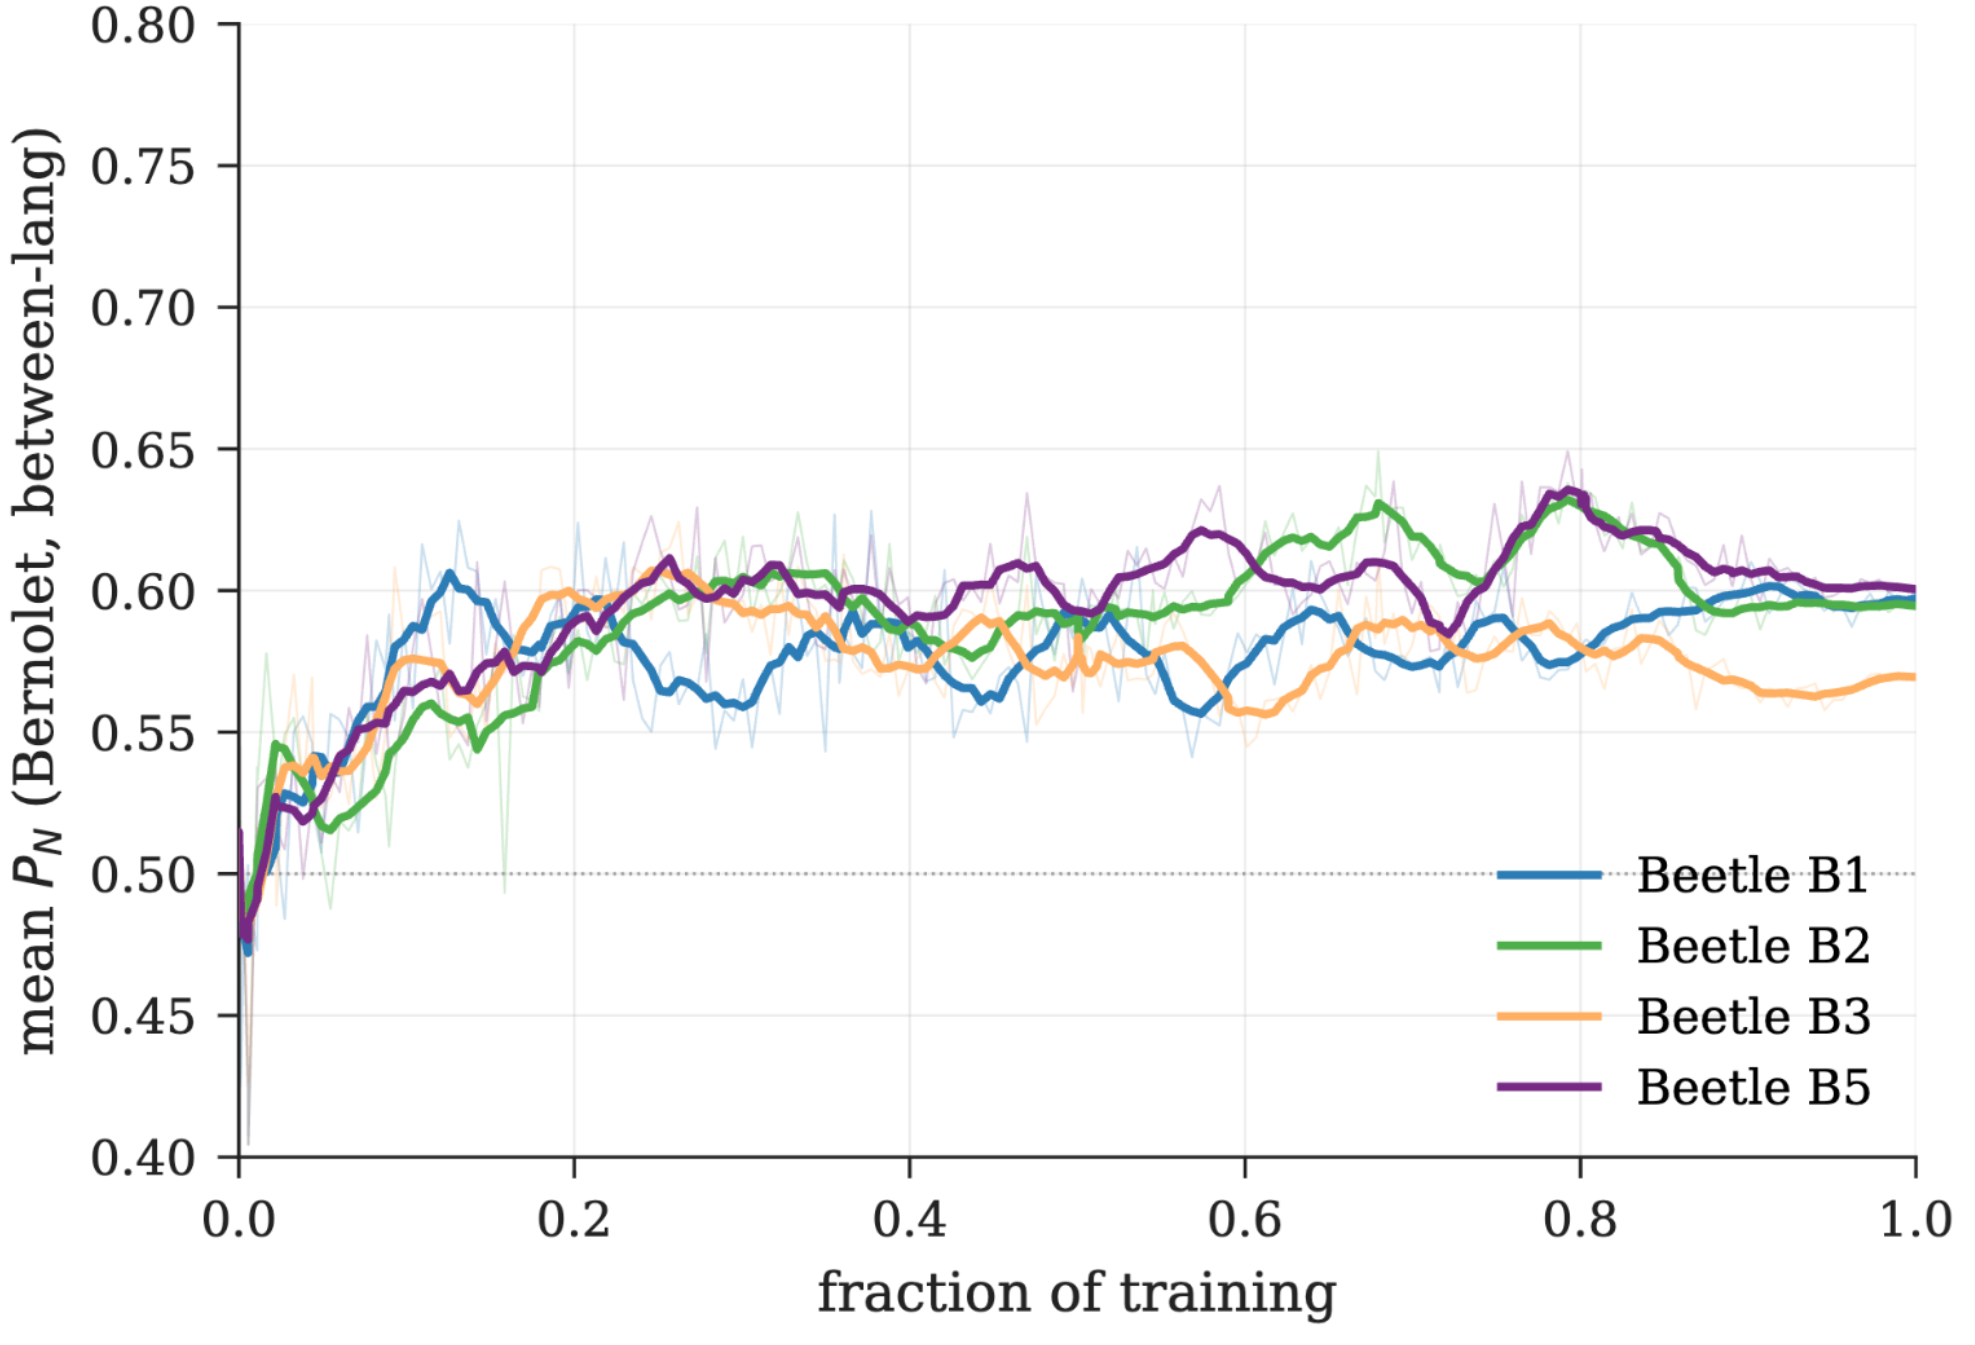
\includegraphics[width=0.5\linewidth]{fig/priming/2.png}
    \caption{Enter Caption}
    \label{fig:placeholder}
\end{figure}


\subsection{Effect of \beetle{} Continual Learning Manipulations}

\begin{figure}
    \centering
    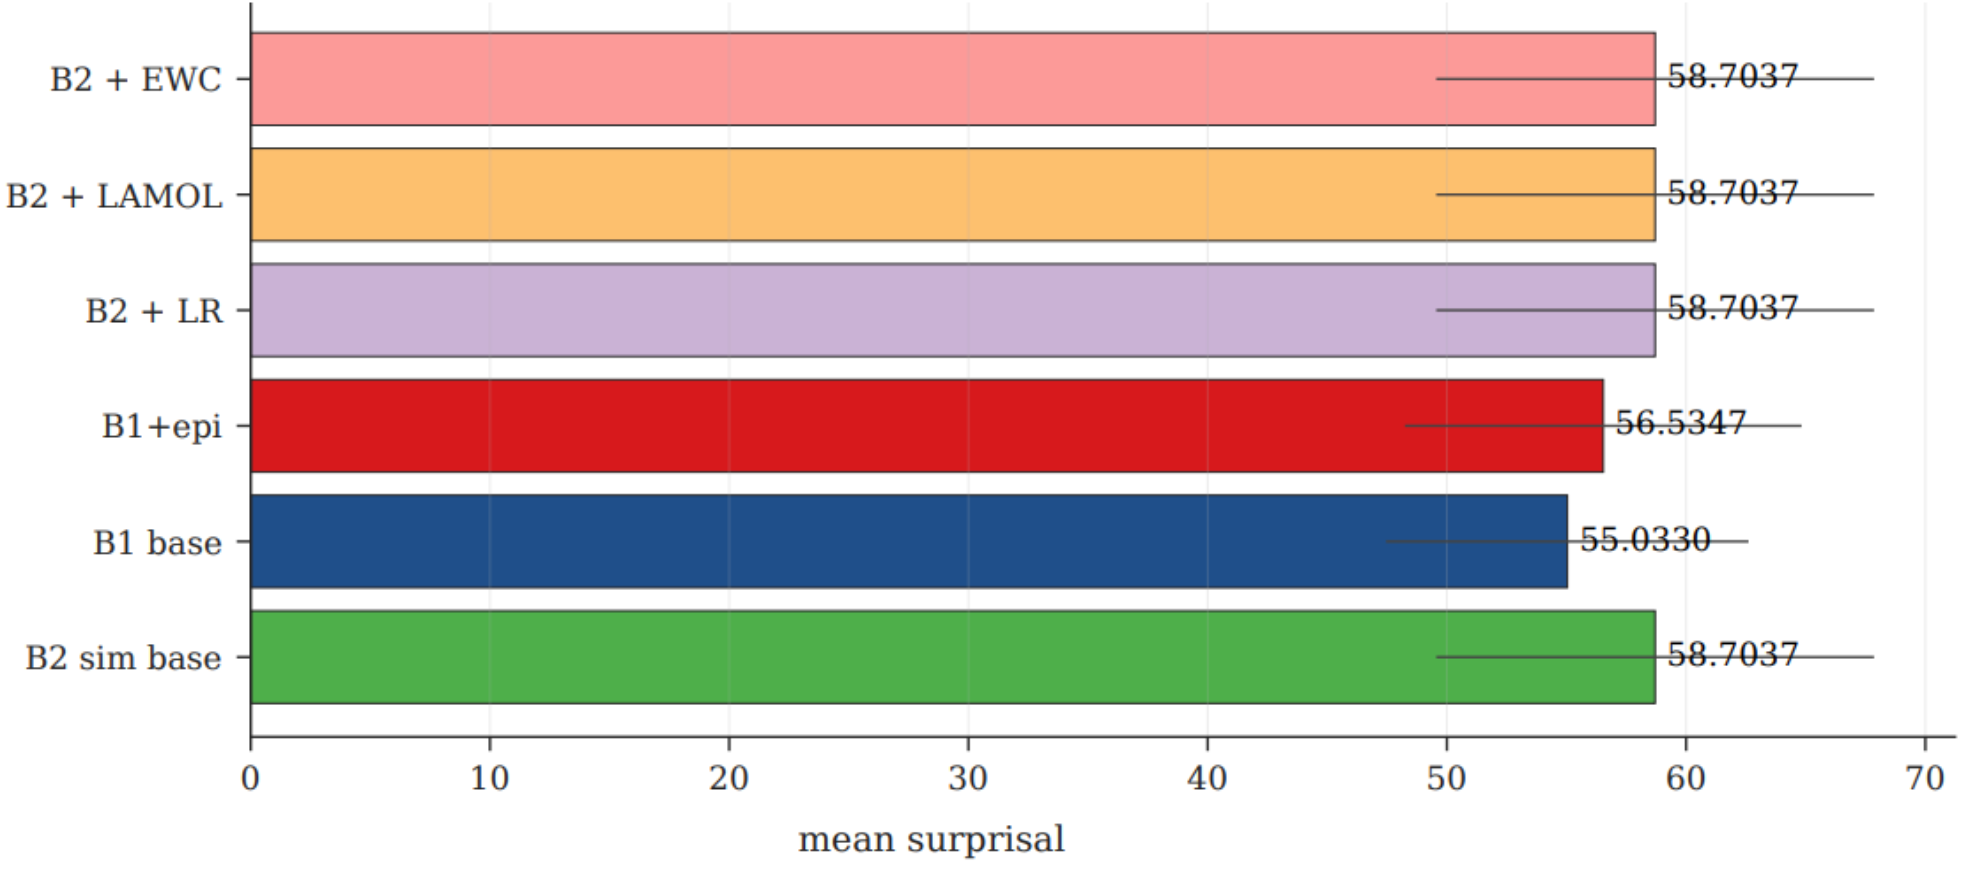
\includegraphics[width=0.5\linewidth]{fig/priming/1.png}
    \caption{Enter Caption}
    \label{fig:placeholder}
\end{figure}

\subsection{Effect of Data Scale on Priming}

Priming effects are better for 24B tokens v Human-Scale. 
\begin{figure}
    \centering
    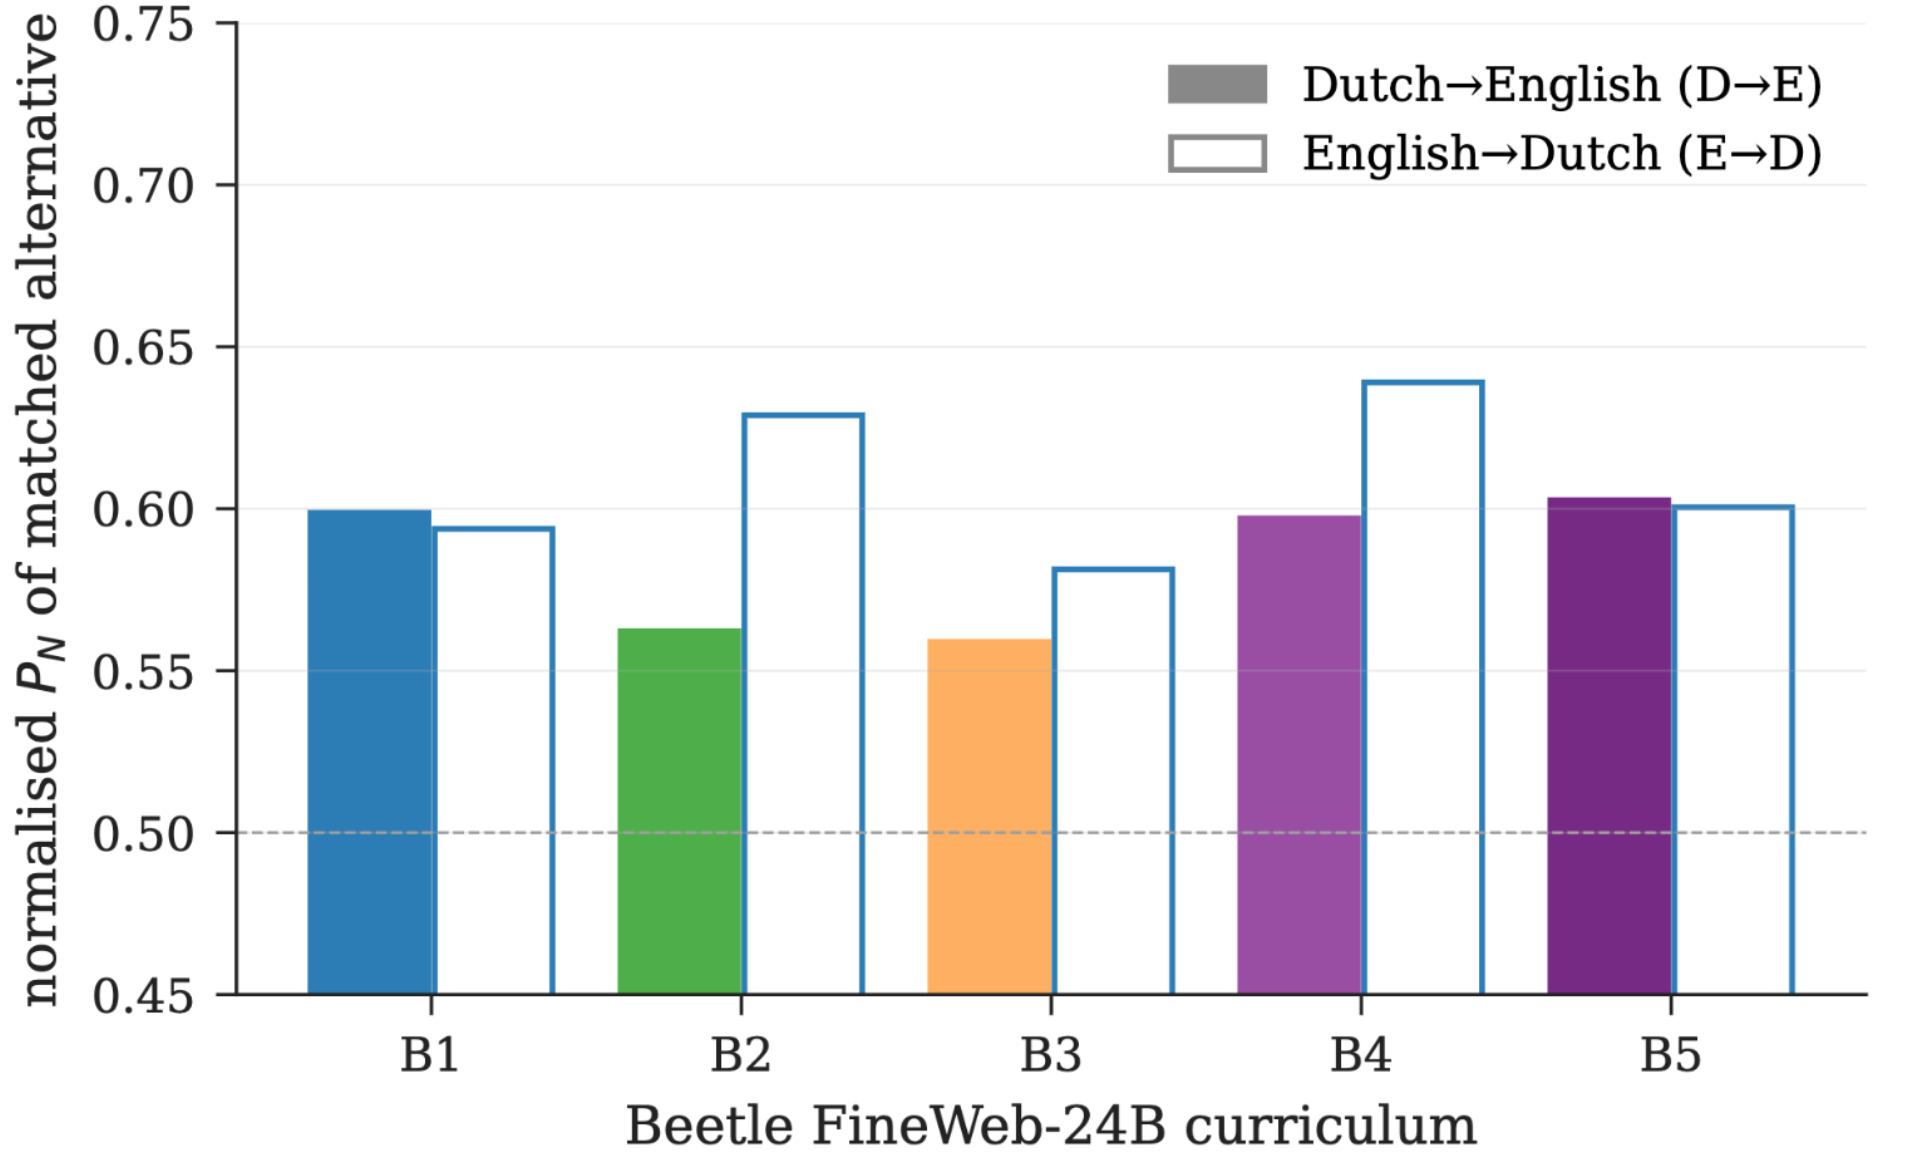
\includegraphics[width=0.5\linewidth]{fig/priming/3.png}
    \caption{Enter Caption}
    \label{fig:placeholder}
\end{figure}

\begin{figure}
    \centering
    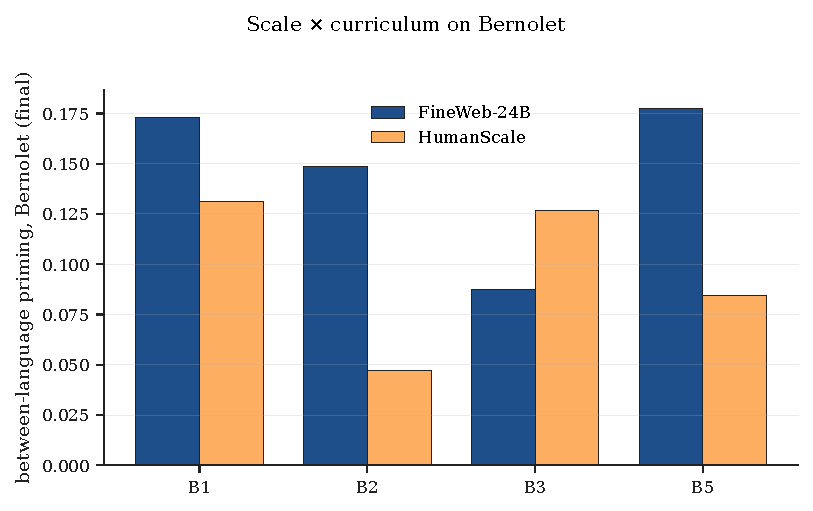
\includegraphics[width=0.5\linewidth]{fig/priming/fig_main_humanscale_bernolet.pdf}
    \caption{Enter Caption}
    \label{fig:placeholder}
\end{figure}



\begin{figure}
    \centering
    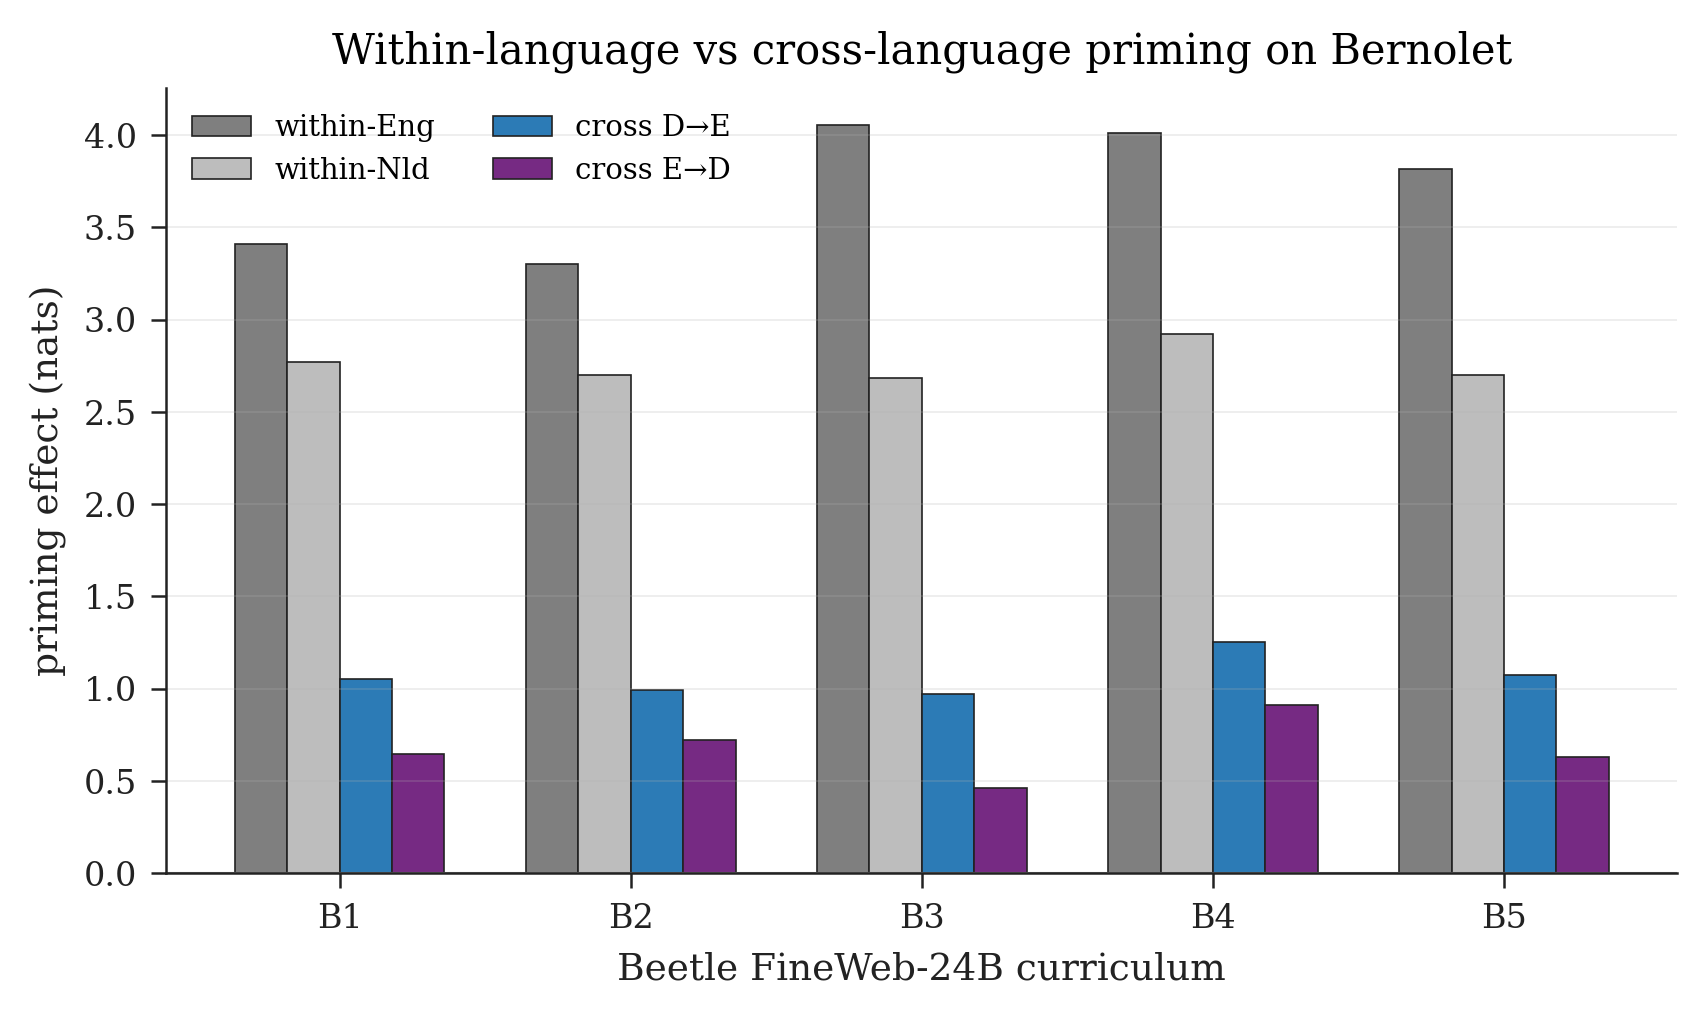
\includegraphics[width=0.5\linewidth]{fig/priming/fig_within_vs_cross_bernolet.png}
    \caption{Enter Caption}
    \label{fig:placeholder}
\end{figure}



\newpage 
\clearpage 
\subsection{Pedagogical supplementary results}\label{appcomp:peda}

Fig.~\ref{fig:ped_panel} and \autoref{tab:headline_pedagogical} summarise the downstream performance \beetle{} 125M parameter models on CLOTH closed-cloze accuracy, RACE zero-shot accuracy, CEFR perplexity gradient, and JFLEG L2-fluency margin, by curriculum and training scale. 


\begin{table*}[!ht]
  \centering
  \scriptsize
  \setlength{\tabcolsep}{4pt}
  \caption{\textbf{Downstream Pedagogical Performance of \beetle{} Models.} CLOTH closed-cloze accuracy, Cambridge open-cloze accuracy, JFLEG learner-fluency margin (bits/token; positive = model prefers corrected over learner-error sentence), false-friend disambiguation margin (bits/token), CEFR-A1 / CEFR-C2 BPT and CEFR gradient (bits between A1 and C2 perplexity). Bold = best per column within the matched-L1 nld--eng family.}
  \label{tab:headline_pedagogical}
  \begin{tabular}{llrrrrrrr}
    \toprule
    Model & Family & CLOTH & Camb.~OC & JFLEG (bits) & FF (bits) & A1 BPT & C2 BPT & A1$\to$C2 grad. \\
    \midrule
    B1 nld--eng     & HS & \textbf{0.380} & \textbf{0.644} & \textbf{0.949} & \textbf{0.585} & 6.572 & 8.818 & 2.247 \\
    B2 nld--eng     & HS & 0.302 & 0.596 & 0.750 & 0.156 & 8.051 & 10.213 & 2.163 \\
    B3-33 nld--eng  & HS & 0.310 & 0.587 & 0.751 & 0.174 & 8.106 & 10.275 & 2.169 \\
    B4 nld--eng     & HS & 0.304 & 0.582 & 0.801 & $-$0.055 & 7.719 & 9.755 & 2.036 \\
    B5 nld--eng     & HS & 0.302 & 0.584 & 0.716 & 0.238 & 8.127 & 10.193 & 2.066 \\
    \midrule
    B1 nld--eng     & FW-2B & 0.369 & 0.638 & 0.833 & 0.457 & 8.851 & 8.614 & $-$0.237 \\
    B2 nld--eng     & FW-2B & 0.322 & 0.567 & 0.502 & 0.238 & 10.317 & 11.047 & 0.730 \\
    B3-33 nld--eng  & FW-2B & 0.329 & 0.614 & 0.511 & 0.235 & 10.354 & 11.056 & 0.702 \\
    B4 nld--eng     & FW-2B & 0.325 & 0.602 & 0.562 & 0.256 & 10.143 & 10.730 & 0.587 \\
    B5 nld--eng     & FW-2B & 0.323 & 0.570 & 0.509 & 0.318 & 10.364 & 11.040 & 0.676 \\
    \midrule
    mono-eng        & HS & 0.369 & 0.659 & 0.888 & 0.351 & 7.297 & 10.558 & \textbf{3.261} \\
    mono-nld        & HS & 0.267 & 0.310 & 0.306 & $-$0.034 & 9.875 & 10.671 & 0.796 \\
    \bottomrule
  \end{tabular}
\end{table*}


\begin{figure}[!ht]
  \centering
  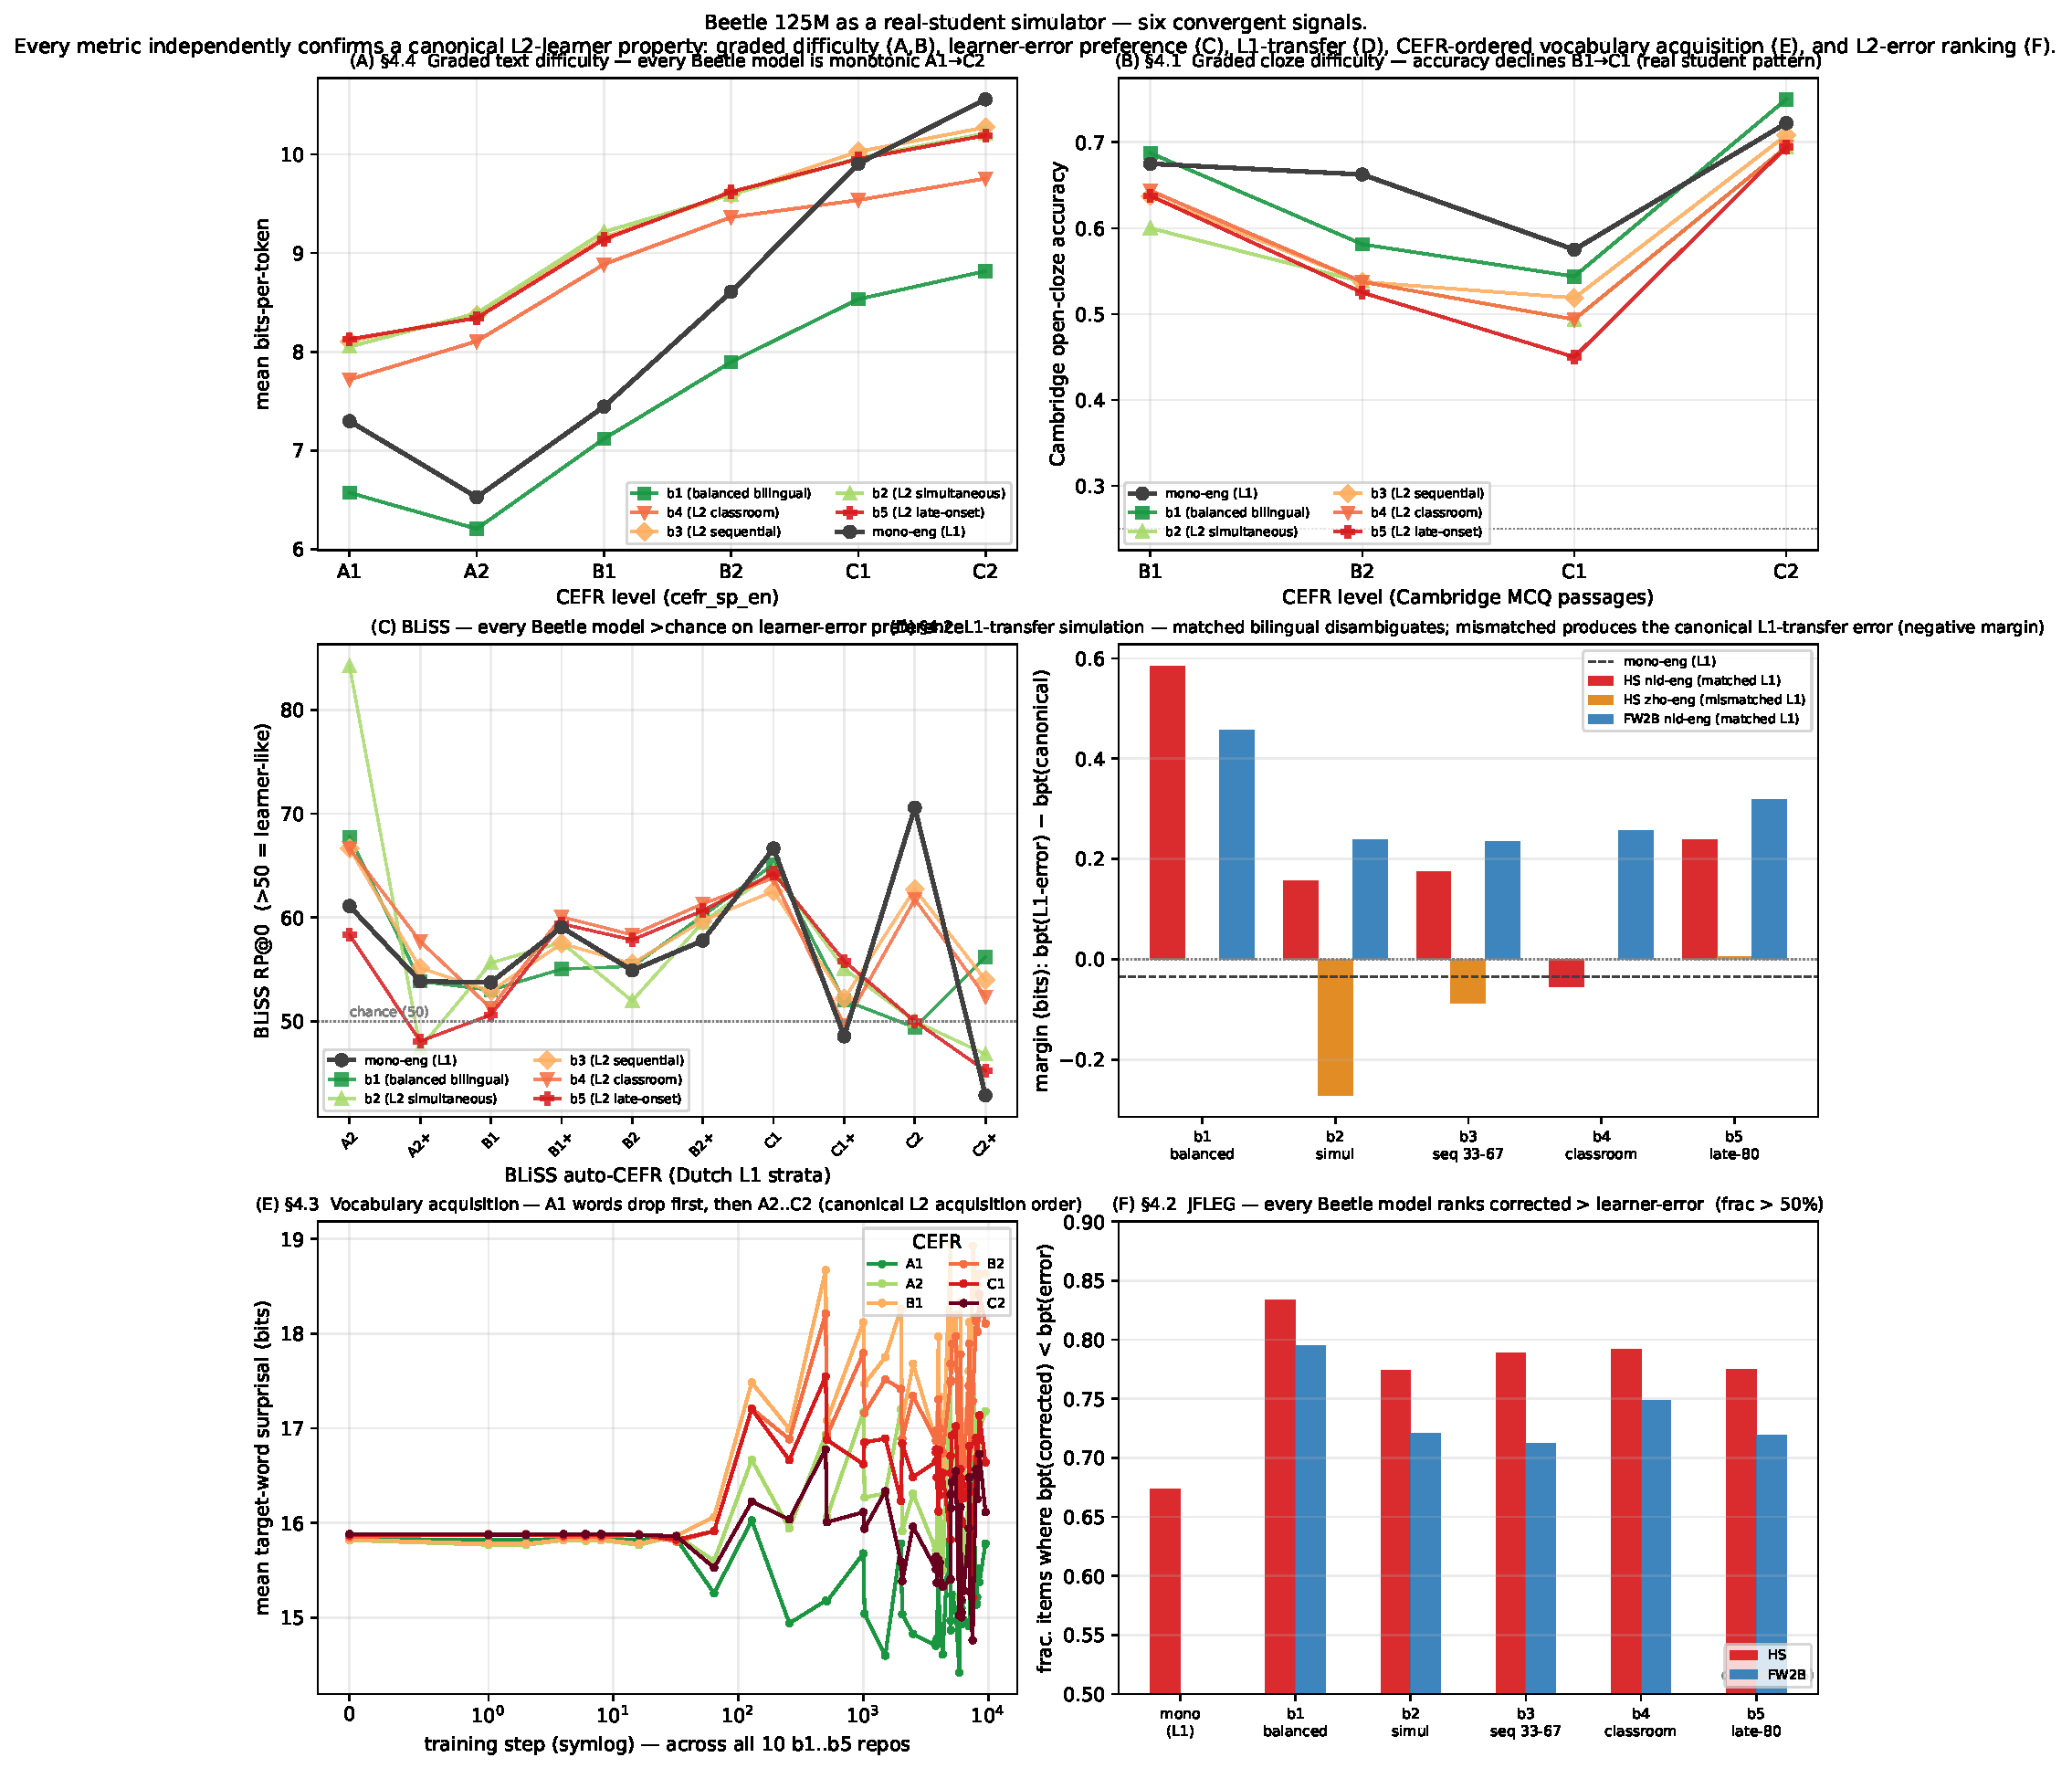
\includegraphics[width=\linewidth]{fig/headline_pedagogical_evidence.pdf}
  \caption{\textbf{Pedagogical evidence panel.} CLOTH closed-cloze accuracy, RACE zero-shot accuracy, CEFR perplexity gradient (A1--C2), and JFLEG L2-fluency margin (matched nld--eng; zho--eng foil) by curriculum and training scale. Companion to body Tab.~\ref{tab:headline_pedagogical}.}
  \label{fig:ped_panel}
\end{figure}


